%% LyX 2.3.7 created this file.  For more info, see http://www.lyx.org/.
%% Do not edit unless you really know what you are doing.
\documentclass[11pt,thmsb]{article}
\usepackage[latin9]{inputenc}
\usepackage{geometry}
\geometry{verbose,tmargin=1in,bmargin=1in,lmargin=1in,rmargin=1in,headheight=1cm,headsep=1cm,footskip=1cm}
\synctex=-1
\usepackage{color}
\usepackage{array}
\usepackage{verbatim}
\usepackage{float}
\usepackage{units}
\usepackage{textcomp}
\usepackage{amsmath}
\usepackage{amsthm}
\usepackage{amssymb}
\usepackage{graphicx}
\usepackage[authoryear]{natbib}

\makeatletter

%%%%%%%%%%%%%%%%%%%%%%%%%%%%%% LyX specific LaTeX commands.
%% Because html converters don't know tabularnewline
\providecommand{\tabularnewline}{\\}

%%%%%%%%%%%%%%%%%%%%%%%%%%%%%% Textclass specific LaTeX commands.
\theoremstyle{plain}
\newtheorem{lem}{\protect\lemmaname}
\theoremstyle{plain}
\newtheorem{thm}{\protect\theoremname}
\theoremstyle{plain}
\newtheorem{cor}{\protect\corollaryname}
\theoremstyle{definition}
\newtheorem{defn}{\protect\definitionname}
\theoremstyle{plain}
\newtheorem{prop}{\protect\propositionname}

%%%%%%%%%%%%%%%%%%%%%%%%%%%%%% User specified LaTeX commands.
%2multibyte Version: 5.50.0.2960 CodePage: 1251
%              Scientific Word   Wrap/Unwrap  Version 2.5             %
%              Scientific Word   Wrap/Unwrap  Version 3.0             %
% If you are separating the files in this message by hand, you will   %
% need to identify the file type and place it in the appropriate      %
% directory.  The possible types are: Document, DocAssoc, Other,      %
% Macro, Style, Graphic, PastedPict, and PlotPict. Extract files      %
% tagged as Document, DocAssoc, or Other into your TeX source file    %
% directory.  Macro files go into your TeX macros directory. Style    %
% files are used by Scientific Word and do not need to be extracted.  %
% Graphic, PastedPict, and PlotPict files should be placed in a       %
% graphics directory.                                                 %
% Graphic files need to be converted from the text format (this is    %
% done for e-mail compatability) to the original 8-bit binary format. %
% Files included:                                                     %
% "/document/NonbalancedJune18.tex", Document, 124302, 6/18/2004, 0:45:10, ""%
% "/document/HZH9JA00.wmf", PastePict, 30602, 6/17/2004, 21:53:40, "" %
% "/document/HZH9JA01.wmf", PastePict, 31310, 6/17/2004, 21:55:05, "" %
% "/document/HZH9JA02.wmf", PastePict, 31498, 6/17/2004, 21:56:09, "" %
% "/document/HXIWF402.wmf", ImportPict, 31112, 6/11/2004, 2:52:58, "" %
% "/document/figure1new.wmf", ImportPict, 8034, 6/11/2004, 2:52:58, ""%
% "/document/HZH9JA03.wmf", PastePict, 49212, 6/11/2004, 2:52:58, ""  %
%%%%%%%%%%%%%%%% Start /document/NonbalancedJune18.tex %%%%%%%%%%%%%%%%


%%%%%%%%%%%%%%%%%%%%%%%%%%%%%%%%%%%%%%%%%%%%%%%%%%%%%%%%%%%%%%%%%%%%%%%%%%%%%%%%%%%%%%%%%%%%%%%%%%%%%%%%%%%%%%%%%%%%%%%%%%%%%%%%%%%%%%%%%%%%%%%%%%%%%%%%%%%%%%%%%%%%%%%%%%%%%%%%%%%%%%%%%%%%%%%%%%%%%%%%%%%%%%%%%%%%%%%%%%%%%%%%%%%%%%%%%%%%%%%%%%%%%%%%%%%%
\usepackage{amsfonts}
\usepackage{version}
\usepackage[font=footnotesize,singlelinecheck=true,format=plain,justification=RaggedRight]{caption}



\setcounter{MaxMatrixCols}{10}
%TCIDATA{TCIstyle=article/art4.lat,lart,article}

%TCIDATA{OutputFilter=LATEX.DLL}
%TCIDATA{Version=5.50.0.2960}
%TCIDATA{Codepage=1251}
%TCIDATA{<META NAME="SaveForMode" CassONTENT="1">}
%TCIDATA{BibliographyScheme=BibTeX}
%TCIDATA{Created=Sat Jul 31 12:49:26 1999}
%TCIDATA{LastRevised=Thursday, July 08, 2021 13:53:15}
%TCIDATA{<META NAME="GraphicsSave" CONTENT="32">}
%TCIDATA{Language=American English}
%TCIDATA{CSTFile=LaTeX article (bright).cst}

\input{tcilatex}
\textwidth 6.2in \textheight 8.65in \setlength{\topmargin}{-0.4in}
\setlength{\oddsidemargin}{0.15in}
\setlength{\evensidemargin}{0.15in}
\usepackage{url}

\usepackage{tikz}
\usepackage{pgfplots}
\usepackage{pgfplotstable}
\pgfplotsset{compat=newest}
\usepgfplotslibrary{dateplot}
\usepgfplotslibrary{groupplots}
\usepgfplotslibrary{fillbetween}
\usepgfplotslibrary{dateplot}

\providecommand{\corollaryname}{Corollary}
\providecommand{\definitionname}{Definition}
\providecommand{\lemmaname}{Lemma}
\providecommand{\propositionname}{Proposition}
\providecommand{\theoremname}{Theorem}



\newcommand{\TS}[1]{{\textcolor{red}{#1}}}
\newcommand{\LPH}[1]{{\textcolor{blue}{#1}}}

\@ifundefined{showcaptionsetup}{}{%
 \PassOptionsToPackage{caption=false}{subfig}}
\usepackage{subfig}
\makeatother

\providecommand{\corollaryname}{Corollary}
\providecommand{\definitionname}{Definition}
\providecommand{\lemmaname}{Lemma}
\providecommand{\propositionname}{Proposition}
\providecommand{\theoremname}{Theorem}


%\usepackage{tikz}
%\usetikzlibrary{external}
\usepackage{xr} % Enable external references
\externaldocument{final_submission_jpe_body}
%\tikzexternalize % Activate externalization
%\tikzsetexternalprefix{figdata/} % Directory for externalized files


\begin{document}
\author{L\'{e}o Aparisi de Lannoy \\
 %EndAName
University of Chicago \and Anmol Bhandari \\
 %EndAName
University of Minnesota \and David Evans \\
 %EndAName
University of Oregon \and Mikhail Golosov \\
 %EndAName
University of Chicago \and Thomas Sargent \\
 %EndAName
NYU}
\title{\textbf{Managing Public Portfolios: Online Appendix}}
\date{October 2024\bigskip{}
}

\maketitle
\bigskip{}
 \bigskip{}

\begin{center}
\textbf{Abstract}
\par\end{center}
This appendix contains the proofs and other details associated with \emph{Managing Public Portfolios}
\newpage{}

\setcounter{page}{1}

\baselineskip0.64cm


\appendix
\pagebreak{}
\setcounter{page}{1}

\vspace{0in}

\section{Additional details for Section \ref{sec: characerization benchmark}\label{sec:Additional-details-for theory}}

\begin{comment}
Let's do a convention that will be very convenient.

$\mathcal{Q}_{t+1,t+k}$ is accumulated discounting between period
$t+1$ and $t+k$, that has a sequence $1$, $1/\mathcal{R}_{t+1,t+2}$,
... for $k=1,2,...$

$Q_{t+1}^{k}$is the interest rate on debt that maturies in period
$t+k+1$. So it has a sequence $1$, $1/R_{t+2}^{rf}$ .... for $k=1,2.$

With this convention, 
\begin{align*}
\sum_{k=1}^{\infty}\overline{\mathcal{Q}_{t+1,t+k}X_{t+k}} & =\overline{X}_{t+1}+\overline{\frac{1}{\mathcal{R}_{t+1,t+2}}}\overline{X}_{t+2}+...\\
 & =\overline{X}_{t+1}+\overline{\frac{1}{R_{t+2}^{rf}}}\overline{X}_{t+2}+...\\
 & =\overline{X}_{t+1}+\overline{Q}_{t+1}^{1}\overline{X}_{t+2}+...\\
 & =\overline{X}_{t+1}+\sum_{k=1}^{\infty}\overline{Q}_{t+1}^{k}\overline{X}_{t+k+1}+...
\end{align*}

So the zeroth order budget consrtaint is 
\[
\overline{X}_{t+1}+\sum_{k=1}^{\infty}\overline{Q}_{t+1}^{k}\overline{X}_{t+k+1}+...=\frac{1}{\overline{Q}_{t}^{1}}\overline{B}_{t}.
\]

In stationary economy, we we have $\overline{Q}_{t+1}^{k}=\beta^{k}$.

We also have in the zeroth order economy that 
\[
\overline{Q}_{t}^{1}\overline{Q}_{t+1}^{k}=\overline{Q}_{t}^{k+1},
\]
so this equation can be written as
\[
\overline{B}_{t}=\overline{Q}_{t}^{1}\overline{X}_{t+1}+\sum_{k=1}^{\infty}\overline{Q}_{t}^{k+1}\overline{X}_{t+k+1}+...
\]

or simply 
\[
\overline{B}_{t}=\sum_{k=1}^{\infty}\overline{Q}_{t}^{k}\overline{X}_{t+k}
\]

In the stationary economy, this gives 
\[
\overline{B}=\sum_{k=1}^{\infty}\beta^{t}\overline{X}=\frac{\beta}{1-\beta}\overline{X}.
\]

Now let's write our budget constraint that we approximate
\[
\mathbb{E}_{t}r_{t+1}^{j}\sum_{k=1}^{\infty}\mathcal{Q}_{t+1,t+k}X_{t+k}=\mathbb{E}_{t}r_{t+1}^{j}\left(R_{t+1}^{rf}+\sum_{i\neq rf}\omega_{t}^{i}r_{t+1}^{i}\right)B_{t}.
\]

The left hand side of this constraint is 
\begin{align*}
LHS & =\frac{1}{2}\mathbb{E}_{t}\partial_{\sigma\sigma}r_{t+1}^{j}\left(\sum_{k=1}^{\infty}\overline{\mathcal{Q}_{t+1,t+k}X_{t+k}}\right)\\
 & +\sum_{k=1}^{\infty}\overline{Q}_{t+1,t+k}\mathbb{E}_{t}\partial_{\sigma}r_{t+1}^{j}\partial_{\sigma}X_{t+k}\\
 & +\sum_{k=1}^{\infty}\overline{Q}_{t+1,t+k}\overline{X}_{t+1,t+k}\mathbb{E}_{t}\partial_{\sigma}r_{t+1}^{j}\partial_{\sigma}\ln\mathcal{Q}_{t+1,t+k}
\end{align*}

The last term is (we have $\overline{Q}_{t+1,t+k+1}=\overline{Q}_{t+1}^{k}$)
\begin{align*}
\sum_{k=1}^{\infty}\overline{Q}_{t+1,t+k}\overline{X}_{t+k}\mathbb{E}_{t}\partial_{\sigma}r_{t+1}^{j}\partial_{\sigma}\ln\mathcal{Q}_{t+1,t+k} & =\sum_{k=2}^{\infty}\overline{Q}_{t+1,t+k}\overline{X}_{t+k}\mathbb{E}_{t}\partial_{\sigma}r_{t+1}^{j}\partial_{\sigma}\ln Q_{t+1}^{k-1}\\
 & =\sum_{k=1}^{\infty}\overline{Q}_{t+1}^{k}\overline{X}_{t+k+1}\mathbb{E}_{t}\partial_{\sigma}r_{t+1}^{j}\partial_{\sigma}\ln Q_{t+1}^{k}
\end{align*}

In the optimum this further have 
\[
\sum_{k=1}^{\infty}\overline{Q}_{t+1,t+k}\mathbb{E}_{t}\partial_{\sigma}r_{t+1}^{j}\partial_{\sigma}X_{t+k}=-\sum_{k=1}^{\infty}\overline{Q}_{t+1,t+k}\overline{G}_{t+k}\mathbb{E}_{t}\partial_{\sigma}r_{t+1}^{j}\partial_{\sigma}\ln G_{t+k}
\]

The right hand side is 
\[
RHS=\frac{1}{2}\mathbb{E}_{t}\partial_{\sigma\sigma}r_{t+1}^{j}\left(\overline{B}_{t}/\overline{Q}_{t}^{1}\right)+\overline{B}_{t}\mathbb{E}_{t}\sum_{i\neq rf}\overline{\omega}_{t}^{i}\partial_{\sigma}r_{t+1}^{j}\partial_{\sigma}r_{t+1}^{i}
\]

So we end up with our final formula
\begin{align*}
\overline{B}_{t}\mathbb{E}_{t}\sum_{i\neq rf}\overline{\omega}_{t}^{i}\partial_{\sigma}r_{t+1}^{j}\partial_{\sigma}r_{t+1}^{i} & \simeq\sum_{k=1}^{\infty}\overline{Q}_{t+1}^{k}\overline{X}_{t+k+1}\mathbb{E}_{t}\partial_{\sigma}r_{t+1}^{j}\partial_{\sigma}\ln Q_{t+1}^{k}\\
 & -\sum_{k=1}^{\infty}\overline{Q}_{t+1}^{k-1}\overline{G}_{t+k}\mathbb{E}_{t}\partial_{\sigma}r_{t+1}^{j}\partial_{\sigma}\ln G_{t+k}.
\end{align*}

Suppose security $j$ is a bond that matured in period $t+1+j$. Then
$r_{t+1}^{j}=Q_{t+1}^{k}/Q_{t}^{k+1}$ and $\mathbb{E}_{t}\partial_{\sigma}r_{t+1}^{j}\partial_{\sigma}r_{t+1}^{i}=\left(\overline{Q_{t+1}^{k}/Q_{t}^{k+1}}\right)\mathbb{E}_{t}\partial_{\sigma}\ln Q_{t+1}^{k}\partial_{\sigma}r_{t+1}^{i}=1/\overline{Q}_{t}^{1}\mathbb{E}_{t}\partial_{\sigma}\ln Q_{t+1}^{k}\partial_{\sigma}r_{t+1}^{i}$.

So now the portfolio that hedges interest rate risk is has entries
like 
\[
s_{t}^{Q,k}=\frac{\overline{Q}_{t+1}^{k}\overline{X}_{t+k+1}}{\overline{B}_{t}/\overline{Q}_{t}^{1}}=\frac{\overline{Q}_{t}^{k+1}\overline{X}_{t+k+1}}{\overline{B}_{t}}.
\]

In stationary equilibrium we have $\overline{X}/\overline{B}=\left(1-\beta\right)\beta^{-1}$,
$\overline{Q}_{t}^{k+1}=\beta^{k+1}$ and so we have $s_{t}^{Q,k}=\left(1-\beta\right)\beta^{k}.$
Sum of this weights is $\sum_{k=1}^{\infty}s_{t}^{Q,k}=\left(1-\beta\right)\frac{\beta}{1-\beta}=\beta$,
and so the share of the risk free bond is $1-\beta$.

So that makes sense. To then the formula is indeed the one that I
have before. If we multiply things by $\overline{Q}_{t}^{1}$, it
gives us 
\begin{align*}
\overline{Q}_{t}^{1}\overline{B}_{t}\mathbb{E}_{t}\sum_{i\neq rf}\overline{\omega}_{t}^{i}\partial_{\sigma}r_{t+1}^{j}\partial_{\sigma}r_{t+1}^{i} & \simeq\sum_{k=1}^{\infty}\overline{Q}_{t}^{k+1}\overline{X}_{t+k+1}\mathbb{E}_{t}\partial_{\sigma}r_{t+1}^{j}\partial_{\sigma}\ln Q_{t+1}^{k}\\
 & -\sum_{k=1}^{\infty}\overline{Q}_{t}^{k}\overline{G}_{t+k}\mathbb{E}_{t}\partial_{\sigma}r_{t+1}^{j}\partial_{\sigma}\ln G_{t+k}.
\end{align*}

So then 
\[
s_{t}^{Q}\left[k\right]=\frac{Q_{t}^{k+1}\mathbb{E}_{t}X_{t+k+1}}{Q_{t}^{1}B_{t}},
\]
\[
s_{t}^{G}\left[k\right]=-\frac{Q_{t}^{k}\mathbb{E}_{t}G_{t+k}}{Q_{t}^{1}B_{t}}.
\]

I see, so with pure discount bonds in stationary economy 
\begin{align*}
\frac{1}{Q_{t}^{1}}\Sigma_{t}^{Q}\omega_{t} & =\Sigma^{Q}s_{t}^{Q}\\
\omega_{t} & =Q_{t}^{1}s_{t}^{Q}=\left[\begin{array}{c}
\frac{Q_{t}^{2}\mathbb{E}_{t}X_{t+2}}{B_{t}}\\
\frac{Q_{t}^{3}\mathbb{E}_{t}X_{t+3}}{B_{t}}\\
\vdots
\end{array}\right].
\end{align*}

In stationary economy $\frac{Q_{t}^{k}\mathbb{E}_{t}X_{t+k}}{B_{t}}=\beta^{k}\left(1-\beta\right)\beta^{-1}=\left(1-\beta\right)\beta^{k-1}$.
So these portfolio weights are $\left[\begin{array}{c}
\left(1-\beta\right)\beta\\
\left(1-\beta\right)\beta^{2}\\
\vdots
\end{array}\right]$ and they sum up to $\beta$.
\end{comment}


\subsection{Proof of Lemma \ref{lem: tax smoothing}(a) \label{subsec:Proof-of-Lemma 1}}

$\overline{\mathcal{R}}_{t+k}=\overline{R}_{t+k}^{rf}$ by Lemma \ref{lem: key asset pricing fact},
so that the zeroth order approximation of equation (\ref{eq: optimality debt level})
implies $\overline{\xi}_{t+k}^{-1}=\overline{\frac{\beta M_{t+k+1}}{M_{t+k}}}\overline{\xi}_{t+k+1}^{-1}\overline{R}_{t+k+1}^{rf}$
for all $k\geq0$. The zeroth order approximation of the households'
optimality condition (\ref{eq: optimality assets}) gives us $1=\overline{\frac{\beta M_{t+k+1}}{M_{t+k}}}\overline{R}_{t+k+1}^{rf}$
for all $k\geq0$. Combine these two equations to show that $\overline{\xi}_{t}=\overline{\xi}_{t+k}$
and, therefore, $\overline{\tau}_{t}=\overline{\tau}_{t+k}$ for all
$k\geq1$.

Multiply equation (\ref{eq: optimality debt level}) for period $t+k$
by $r_{t+1}^{j}$ and take the expectation in period $t$ to get 
\begin{equation}
\mathbb{E}_{t}\frac{1}{\xi_{t+k}}r_{t+1}^{j}=\mathbb{E}_{t}\frac{\beta M_{t+k+1}}{M_{t+k}}\frac{1}{\xi_{t+k+1}}\mathcal{R}_{t+k+1}r_{t+1}^{j}.\label{eq: app debt smoothing r}
\end{equation}
Lemma \ref{lem: key asset pricing fact} implies that $\mathbb{E}_{t}\partial_{\sigma}\mathcal{R}_{t+k+1}\partial_{\sigma}r_{t+1}^{i}$=$\mathbb{E}_{t}\partial_{\sigma}R_{t+k+1}^{rf}\partial_{\sigma}r_{t+1}^{i}$,
so that the second order approximation of (\ref{eq: app debt smoothing r})
is 
\begin{align*}
 & \mathbb{E}_{t}\partial_{\sigma}\frac{1}{\xi_{t+k}}\partial_{\sigma}r_{t+1}^{j}+\frac{1}{2}\frac{1}{\overline{\xi}_{t+k}}\mathbb{E}_{t}\partial_{\sigma\sigma}r_{t+1}^{j}\\
= & \overline{\frac{\beta M_{t+k+1}}{M_{t+k}}}\frac{1}{\overline{\xi}_{t+k+1}}\mathbb{E}_{t}\partial_{\sigma}R_{t+k+1}^{rf}\partial_{\sigma}r_{t+1}^{j}+\overline{\frac{\beta M_{t+k+1}}{M_{t+k}}}\overline{R}_{t+k+1}^{rf}\mathbb{E}_{t}\partial_{\sigma}\frac{1}{\xi_{t+k+1}}\partial_{\sigma}r_{t+1}^{j}\\
 & +\frac{\overline{R}_{t+k+1}^{rf}}{\overline{\xi}_{t+k+1}}\mathbb{E}_{t}\partial_{\sigma}\frac{\beta M_{t+k+1}}{M_{t+k}}\partial_{\sigma}r_{t+1}^{j}+\frac{1}{2}\overline{\frac{\beta M_{t+k+1}}{M_{t+k}}}\frac{\overline{R}_{t+k+1}^{rf}}{\overline{\xi}_{t+k+1}}\mathbb{E}_{t}\partial_{\sigma\sigma}r_{t+1}^{j}.
\end{align*}
From the results obtained in the previous paragraph, we know that
$\overline{\xi}_{t+k}=\overline{\xi}_{t}$ and $\partial_{\sigma}\frac{1}{\xi_{t+k}}=-\frac{\partial_{\sigma}\tau_{t+k}}{\xi^{\prime}\left(\overline{\tau}_{t}\right)}$
and that $\overline{\frac{\beta M_{t+k+1}}{M_{t+k}}}\overline{R}_{t+k+1}^{rf}=1$,
so that this equation further simplifies to 
\begin{align*}
-\frac{\xi^{\prime}\left(\overline{\tau}_{t}\right)}{\xi\left(\overline{\tau}_{t}\right)}\mathbb{E}_{t}\partial_{\sigma}\tau_{t+k}\partial_{\sigma}r_{t+1}^{j}+\frac{1}{2}\mathbb{E}_{t}\partial_{\sigma\sigma}r_{t+1}^{j} & =\mathbb{E}_{t}\partial_{\sigma}\ln R_{t+k+1}^{rf}\partial_{\sigma}r_{t+1}^{j}-\mathbb{E}_{t}\partial_{\sigma}\tau_{t+k+1}\partial_{\sigma}r_{t+1}^{j}\\
 & +\mathbb{E}_{t}\partial_{\sigma}\ln\frac{\beta M_{t+k+1}}{M_{t+k}}\partial_{\sigma}r_{t+1}^{j}+\frac{1}{2}\mathbb{E}_{t}\partial_{\sigma\sigma}r_{t+1}^{j}.
\end{align*}
Similarly, the household optimality condition (\ref{eq: optimality assets})
implies that $\mathbb{E}_{t}r_{t+1}^{j}=\mathbb{E}_{t}\frac{\beta M_{t+k+1}}{M_{t+k}}R_{t+k+1}^{rf}r_{t+1}^{j}$,
which to the second order of approximation gives 
\begin{align*}
\frac{1}{2}\mathbb{E}_{t}\partial_{\sigma\sigma}r_{t+1}^{j}= & \mathbb{E}_{t}\partial_{\sigma}\ln R_{t+k+1}^{rf}\partial_{\sigma}r_{t+1}^{j}+\mathbb{E}_{t}\partial_{\sigma}\ln\frac{\beta M_{t+k+1}}{M_{t+k}}\partial_{\sigma}r_{t+1}^{j}+\frac{1}{2}\mathbb{E}_{t}\partial_{\sigma\sigma}r_{t+1}^{j}.
\end{align*}
Combine these two equations to show that $\mathbb{E}_{t}\partial_{\sigma}\tau_{t+k}\partial_{\sigma}r_{t+1}^{j}=\mathbb{E}_{t}\partial_{\sigma}\tau_{t+k+1}\partial_{\sigma}r_{t+1}^{j}$
for all $k$, $j$.

\subsection{Proof of Theorem \ref{thm: benchmark}}

We first consider the zeroth order economy. Using the definition of
zero coupon bond prices, we have 
\[
\overline{Q}_{t}^{k}=\frac{\overline{S}_{t+1}}{\overline{S}_{t}}\times\frac{\overline{S}_{t+2}}{\overline{S}_{t+1}}\times...\times\frac{\overline{S}_{t+k}}{\overline{S}_{t+k-1}}=\overline{Q}_{t}^{1}\times\overline{Q}_{t+1}^{1}\times...\times\overline{Q}_{t+k-1}^{1}=\overline{Q}_{t}^{1}\overline{Q}_{t+1}^{k-1}.
\]
Furthermore, Lemma \ref{lem: key asset pricing fact} implies that
excess returns are zero to the zeroth order and $\mathcal{\overline{Q}}_{t+1,t+k}=\overline{Q}_{t+1}^{k-1}$.
Thus, the budget constraint (\ref{eq: budget constraint govt PV})
gives us
\begin{equation}
\overline{B}_{t}/\overline{Q}_{t}^{1}=\sum_{k=1}^{\infty}\overline{Q}_{t+1}^{k-1}\overline{X}_{t+k}\quad\Longrightarrow\quad\overline{B}_{t}=\sum_{k=1}^{\infty}\overline{Q}_{t}^{k}\overline{X}_{t+k},\label{eq: app budget constraint govt PV 0th}
\end{equation}
where we used a convention that $\overline{Q}_{t}^{0}=1$. We have
$\overline{X}_{t+k}=\overline{T}_{t+k}-\overline{G}_{t+k}$ and Lemma
\ref{lem: tax smoothing} implies that in the optimum $\overline{T}_{t+k}=\overline{T}_{t}$
for all $k$. This allows us to solve for the optimal level of tax
revenues, $\overline{T}_{t}=(\overline{B}_{t}+\sum_{k=1}^{\infty}\overline{Q}_{t}^{k}\overline{G}_{t+k})/\sum_{k=1}^{\infty}\overline{Q}_{t}^{k}$.

Multiply (\ref{eq: budget constraint govt PV}) by $r_{t+1}^{j}$
and take period $t$ expectations to write it as 
\[
\mathbb{E}_{t}r_{t+1}^{j}\sum_{k=1}^{\infty}\mathcal{Q}_{t+1,t+k}X_{t+k}=\mathbb{E}_{t}r_{t+1}^{j}\left(R_{t+1}^{rf}+\sum_{i\neq rf}\omega_{t}^{i}r_{t+1}^{i}\right)B_{t}.
\]
The second order approximations of the right hand side and the left
hand side of this equation, due to Lemma \ref{lem: key asset pricing fact},
are 
\[
RHS\simeq\frac{1}{2}\frac{\overline{B}_{t}}{\overline{Q}_{t}^{1}}\mathbb{E}_{t}\partial_{\sigma\sigma}r_{t+1}^{j}+\overline{B}_{t}\sum_{i\neq rf}\overline{\omega}_{t}^{i}\mathbb{E}_{t}\partial_{\sigma}r_{t+1}^{j}\partial_{\sigma}r_{t+1}^{i}
\]
and 
\begin{align*}
LHS & \simeq\frac{1}{2}\left(\sum_{k=1}^{\infty}\overline{Q}_{t+1}^{k-1}\overline{X}_{t+k}\right)\mathbb{E}_{t}\partial_{\sigma\sigma}r_{t+1}^{j}+\sum_{k=1}^{\infty}\overline{Q}_{t+1}^{k-1}\mathbb{E}_{t}\partial_{\sigma}r_{t+1}^{j}\partial_{\sigma}X_{t+k}+\sum_{k=1}^{\infty}\overline{Q}_{t+1}^{k-1}\overline{X}_{t+k}\mathbb{E}_{t}\partial_{\sigma}r_{t+1}^{j}\partial_{\sigma}\ln\mathcal{Q}_{t+1,t+k}.
\end{align*}

We want to make several observations about these equations. First,
the first terms on the right hand sides of these two equations are
equal, due to (\ref{eq: app budget constraint govt PV 0th}). Second,
$\mathbb{E}_{t}\partial_{\sigma}r_{t+1}^{j}\partial_{\sigma}\ln\mathcal{Q}_{t+1,t+1}=0$
since $\mathcal{Q}_{t+1,t+1}=1$, and $\mathbb{E}_{t}\partial_{\sigma}r_{t+1}^{j}\partial_{\sigma}\ln\mathcal{Q}_{t+1,t+k}=\mathbb{E}_{t}\partial_{\sigma}r_{t+1}^{j}\partial_{\sigma}\ln Q_{t+1}^{k-1}$
for $k>1$ due to Lemma \ref{lem: key asset pricing fact}. Therefore,
combining these equations and multiplying both sides by $\overline{Q}_{t}^{1}$
we have 
\begin{align}
\overline{Q}_{t}^{1}\overline{B}_{t}\sum_{i\neq rf}\overline{\omega}_{t}^{i}\mathbb{E}_{t}\partial_{\sigma}r_{t+1}^{j}\partial_{\sigma}r_{t+1}^{i} & =\sum_{k=1}^{\infty}\overline{Q}_{t}^{k+1}\overline{X}_{t+k+1}\mathbb{E}_{t}\partial_{\sigma}r_{t+1}^{j}\partial_{\sigma}\ln Q_{t+1}^{k}\label{eq: app budget constraint govt PV 2nd}\\
 & +\sum_{k=1}^{\infty}\overline{Q}_{t}^{k}\overline{G}_{t+k}\mathbb{E}_{t}\partial_{\sigma}r_{t+1}^{j}\partial_{\sigma}\ln G_{t+k}+\sum_{k=1}^{\infty}\overline{Q}_{t}^{k}\mathbb{E}_{t}\partial_{\sigma}r_{t+1}^{j}\partial_{\sigma}T_{t+k}.\nonumber 
\end{align}
Note that $T_{t+k}$ is only a function of tax rate $\tau_{t+k},$
so we can write $T_{t+k}=T\left(\tau_{t+k}\right)$ and $\partial_{\sigma}T_{t+k}=T^{\prime}\left(\overline{\tau}_{t+k}\right)\partial_{\sigma}\tau_{t+k}$.
But then we have 
\begin{align}
\mathbb{E}_{t}\partial_{\sigma}r_{t+1}^{j}\partial_{\sigma}T_{t+k} & =T^{\prime}\left(\overline{\tau}_{t+k}\right)\mathbb{E}_{t}\partial_{\sigma}r_{t+1}^{j}\partial_{\sigma}\tau_{t+k}=T^{\prime}\left(\overline{\tau}_{t}\right)\mathbb{E}_{t}\partial_{\sigma}r_{t+1}^{j}\partial_{\sigma}\tau_{t+1}\label{eq: app tax smoothing and portfolio}
\end{align}
where the second equality follows from Lemma \ref{lem: tax smoothing}(a).
Finally, observe that the last equation in (\ref{eq: app tax smoothing and portfolio})
must be equal to zero by Lemma \ref{lem: tax smoothing}(b), which
establishes (\ref{eq: main result benchmark}).

\subsection{Proof of Corollary \ref{lem: portfolio reform}}

Observe that in the proof of Theorem \ref{thm: benchmark} upto equation
(\ref{eq: app tax smoothing and portfolio}) we only used first order
properties of the debt level optimality condition\footnote{This follows since we always pre-multiplied it by $r_{t+1}^{j}$ prior
to taking second order expansions, and $\overline{r}_{t+1}^{j}=0$
by Lemma \ref{lem: key asset pricing fact}.} (\ref{eq: optimality debt level}), and did not use portfolio optimality
condition (\ref{eq: optimality portfolio}) at all. Without invoking
this optimality condition, the government budget constraint is 
\begin{align*}
\overline{Q}_{t}^{1}\overline{B}_{t}\sum_{i\neq rf}\overline{\omega}_{t}^{i}\mathbb{E}_{t}\partial_{\sigma}r_{t+1}^{j}\partial_{\sigma}r_{t+1}^{i} & =\sum_{k=1}^{\infty}\overline{Q}_{t}^{k+1}\overline{X}_{t+k+1}\mathbb{E}_{t}\partial_{\sigma}r_{t+1}^{j}\partial_{\sigma}\ln Q_{t+1}^{k}\\
 & +\sum_{k=1}^{\infty}\overline{Q}_{t}^{k}\overline{G}_{t+k}\mathbb{E}_{t}\partial_{\sigma}r_{t+1}^{j}\partial_{\sigma}\ln G_{t+k}+T^{\prime}\left(\overline{\tau}_{t}\right)\left(\sum_{k=1}^{\infty}\overline{Q}_{t}^{k}\right)\mathbb{E}_{t}\partial_{\sigma}r_{t+1}^{j}\partial_{\sigma}\tau_{t+1}.
\end{align*}
Using definition of $\overline{\omega}_{t}^{*}$, this implies that
\begin{align*}
\sum_{i\neq rf}\left(\overline{\omega}_{t}^{i}-\overline{\omega}_{t}^{*,i}\right)\mathbb{E}_{t}\partial_{\sigma}r_{t+1}^{j}\partial_{\sigma}r_{t+1}^{i} & =\frac{T^{\prime}\left(\overline{\tau}_{t}\right)\left(\sum_{k=1}^{\infty}\overline{Q}_{t}^{k}\right)}{\overline{Q}_{t}^{1}\overline{B}_{t}}\mathbb{E}_{t}\partial_{\sigma}r_{t+1}^{j}\partial_{\sigma}\tau_{t+1}.
\end{align*}

Taking the second order approximation of (\ref{eq: perturbation portfolio}),
we obtain 
\[
\partial_{\sigma\sigma}\partial_{prfl,j}V=\beta^{t}\Pr\left(s^{t}\right)\overline{M}_{t+1}\frac{\xi^{\prime}\left(\overline{\tau}_{t+1}\right)}{\xi\left(\overline{\tau}_{t+1}\right)^{2}}\mathbb{E}_{t}\partial_{\sigma}\tau_{t+1}\partial_{\sigma}r_{t+1}^{j}.
\]
Combining these two expressions, and using zeroth order tax smoothing
$\overline{\tau}_{t}=\overline{\tau}_{t+1}$, we get 
\[
\sum_{i\neq rf}\left(\overline{\omega}_{t}^{*,i}-\overline{\omega}_{t}^{i}\right)\mathbb{E}_{t}\partial_{\sigma}r_{t+1}^{j}\partial_{\sigma}r_{t+1}^{i}=\underbrace{\frac{T^{\prime}\left(\overline{\tau}_{t}\right)\xi\left(\overline{\tau}_{t}\right)^{2}}{-\xi^{\prime}\left(\overline{\tau}_{t}\right)\overline{B}_{t}}\frac{\sum_{k=1}^{\infty}\overline{Q}_{t}^{k}/\overline{Q}_{t}^{1}}{\beta^{t}\Pr\left(s^{t}\right)\overline{M}_{t+1}}}_{const_{t}}\partial_{\sigma\sigma}\partial_{prfl,j}V,
\]
which is the expression stated in Corollary \ref{lem: portfolio reform}.
Note that $const_{t}>0$ if $\overline{B}_{t}>0$, $-\xi^{\prime}\left(\overline{\tau}_{t}\right)>0$,
and $T^{\prime}\left(\overline{\tau}_{t}\right)=\xi\left(\overline{\tau}_{t}\right)\overline{Y}_{t}>0$.
If $v$ is constant elasticity $\gamma$ then $\xi\left(\tau\right)=1-\gamma\frac{\tau}{1-\tau}$
and the peak of the Laffer curve $\tau^{*}$ satisfies $\frac{\tau^{*}}{1-\tau^{*}}=\frac{1}{\gamma}$.
This implies that if $\tau<\tau^{*}$ then $\xi\left(\tau\right),-\xi^{\prime}\left(\tau\right)>0$.

\section{Additional details for Section \ref{sec:Extensions} \label{sec:Additional-details-for extentions}}

\subsection{Additional details for Section \ref{sec: tax revenue risk}}

First of all, observe that since $\xi_{t}$ is the transformation
of $\tau_{t}$ the proof of Lemma \ref{lem: tax smoothing} remains
unchanged. This implies that $\overline{\tau}_{t+k}=\overline{\tau}_{t}$
for all $t$ and $\overline{\tau}_{t}$ is the solution to $\overline{B}_{t}=\sum_{k=1}^{\infty}\overline{Q}_{t}^{k}(\overline{\Theta}_{t+k}\left(\overline{\tau}_{t}\left(1-\overline{\tau_{t}}\right)\right)-\overline{G}_{t+k})$
which is the generalization of equation (\ref{eq: app budget constraint govt PV 0th}).
Let $\overline{T}_{t+k}^{tax}=\overline{\Theta}_{t+k}\overline{\tau}_{t}\left(1-\overline{\tau_{t}}\right)$.
We have 
\[
\mathbb{E}_{t}\partial_{\sigma}r_{t+1}^{j}\partial_{\sigma}T_{t+k}=\mathbb{E}_{t}\partial_{\sigma}r_{t+1}^{j}\partial_{\sigma}T_{t+k}^{tax}=\overline{T}_{t+k}\mathbb{E}_{t}\partial_{\sigma}r_{t+1}^{j}\partial_{\sigma}\ln\Theta_{t+k}+\overline{\Theta}_{t+k}\underbrace{\mathbb{E}_{t}\partial_{\sigma}r_{t+1}^{j}\partial_{\sigma}\overline{\tau}_{t}\left(1-\overline{\tau_{t}}\right)}_{=0},
\]
where the last term is zero following the same steps as in (\ref{eq: app tax smoothing and portfolio}).
Substitute this equation into (\ref{eq: app budget constraint govt PV 2nd})
to obtain the expression for the optimal portfolio $\overline{\omega}_{t}$.
If $\Sigma_{t}$ matrix is invertible, it can be written as (\ref{eq: w* TFP}).

\subsection{Additional details for Section \ref{sec: liquidity}}

In the economy with liquidity premia, the second order approximation
of portfolio optimality condition, equation (\ref{eq: optimality portfolio appr}),
holds but the analogue of equation (\ref{eq: optimality portfolio appr HH})
becomes
\[
\frac{1}{2}\overline{\frac{\beta M_{t+1}}{M_{t}}}\mathbb{E}_{t}\partial_{\sigma\sigma}r_{t+1}^{j}+\mathbb{E}_{t}\partial_{\sigma}r_{t+1}^{j}\partial_{\sigma}\frac{\beta M_{t+1}}{M_{t}}=-\frac{1}{2}\partial_{\sigma\sigma}\left(w_{t,k}-w_{t,1}\right).
\]
Combining this equation with (\ref{eq: optimality portfolio appr})
we obtain 
\[
\frac{1}{2}\partial_{\sigma\sigma}\left(w_{t,k}-w_{t,1}\right)=\overline{\frac{\beta M_{t+1}}{M_{t}}}\mathbb{E}_{t}\partial_{\sigma}r_{t+1}^{j}\partial_{\sigma}\frac{1}{\xi_{t+1}}=\frac{-\xi^{\prime}\left(\overline{\tau}_{t+1}\right)}{\xi\left(\overline{\tau}_{t+1}\right)}\overline{\frac{\beta M_{t+1}}{M_{t}}}\mathbb{E}_{t}\partial_{\sigma}r_{t+1}^{j}\partial_{\sigma}\tau_{t+1}.
\]
Since to the first order the liquidity premium is zero, conclusions
of Lemma \ref{lem: tax smoothing}(a) extend to this economy, which
allows us to write the above equation as 
\begin{equation}
\mathbb{E}_{t}\partial_{\sigma}r_{t+1}^{j}\partial_{\sigma}\tau_{t+1}=\frac{\xi\left(\overline{\tau}_{t}\right)}{-\xi^{\prime}\left(\overline{\tau}_{t}\right)\overline{Q}_{t}^{1}}\frac{1}{2}\partial_{\sigma\sigma}\left(w_{t,k}-w_{t,1}\right).\label{eq: tax smoothing appr liquidity}
\end{equation}
Equation (\ref{eq: app tax smoothing and portfolio}) still holds
but when we combine it with the portfolio optimality condition (\ref{eq: tax smoothing appr liquidity})
we obtain
\[
\mathbb{E}_{t}\partial_{\sigma}r_{t+1}^{j}\partial_{\sigma}T_{t+k}=T^{\prime}\left(\overline{\tau}_{t}\right)\frac{\xi\left(\overline{\tau}_{t}\right)^{2}}{-\xi^{\prime}\left(\overline{\tau}_{t}\right)\overline{Q}_{t}^{1}}\frac{1}{2}\partial_{\sigma\sigma}\left(w_{t,k}-w_{t,1}\right)=\frac{\overline{Y}_{t}\xi\left(\overline{\tau}_{t}\right)^{2}}{-\xi^{\prime}\left(\overline{\tau}_{t}\right)\overline{Q}_{t}^{1}}\frac{1}{2}\partial_{\sigma\sigma}\left(w_{t,k}-w_{t,1}\right).
\]
Substitute this equation into (\ref{eq: app budget constraint govt PV 2nd})
to get 
\begin{align}
\overline{Q}_{t}^{1}\overline{B}_{t}\sum_{i\neq rf}\overline{\omega}_{t}^{i}\mathbb{E}_{t}\partial_{\sigma}r_{t+1}^{j}\partial_{\sigma}r_{t+1}^{i} & =\sum_{k=1}^{\infty}\overline{Q}_{t}^{k+1}\overline{X}_{t+k+1}\mathbb{E}_{t}\partial_{\sigma}r_{t+1}^{j}\partial_{\sigma}\ln Q_{t+1}^{k}\label{eq: optimal portfolio appr liquidity}\\
 & +\sum_{k=1}^{\infty}\overline{Q}_{t}^{k}\overline{G}_{t+k}\mathbb{E}_{t}\partial_{\sigma}r_{t+1}^{j}\partial_{\sigma}\ln G_{t+k}+\frac{\overline{Y}_{t}\xi\left(\overline{\tau}_{t}\right)^{2}\sum_{k=1}^{\infty}\overline{Q}_{t}^{k}}{-\xi^{\prime}\left(\overline{\tau}_{t}\right)\overline{Q}_{t}^{1}}\frac{1}{2}\partial_{\sigma\sigma}\left(w_{t,k}-w_{t,1}\right).\nonumber 
\end{align}
This is equation (\ref{eq: w* liquidity}) when $\Sigma_{t}$ is invertible.

To derive (\ref{eq: liquidity from data}), it will be useful to write
household optimality conditions (\ref{eq: optimality assets liquidity})
in a slightly different form. Consider a perturbation in which households
change the quantity of holding a $k$ period bond by an infinitesimal
amount until maturity of that bond. The implied optimality condition
for that perturbation is 
\[
M_{t}Q_{t}^{k}=\mathbb{E}_{t}\beta^{k}M_{t+k}+M_{t}Q_{t}^{k}w_{t,k}+\mathbb{E}_{t}M_{t+1}Q_{t+1}^{k-1}w_{t+1,k-1}+...+\mathbb{E}_{t}M_{t+k-1}Q_{t+k-1}^{1}w_{t+k-1,1}.
\]
The optimality condition for the notional private $k$ period bond
is $M_{t}Q_{t}^{k,pr}=\mathbb{E}_{t}\beta^{k}M_{t+k}$, which implies
\[
0=\left(\frac{1}{Q_{t}^{k}}-\frac{1}{Q_{t}^{k,pr}}\right)\mathbb{E}_{t}\frac{\beta^{k}M_{t+k}}{M_{t}}+w_{t,k}+\mathbb{E}_{t}\frac{\beta M_{t+1}}{M_{t}}\frac{Q_{t+1}^{k-1}}{Q_{t}^{k}}w_{t+1,k-1}+...+\mathbb{E}_{t}\frac{\beta^{k-1}M_{t+k-1}}{M_{t}}\frac{Q_{t+k-1}^{1}}{Q_{t}^{k}}w_{t+k-1,1}.
\]
Take the second order approximation of this equation and use the fact
that to the first order liquidity premia is zero to obtain 
\[
0=\partial_{\sigma\sigma}\left(\frac{1}{Q_{t}^{k}}-\frac{1}{Q_{t}^{k,pr}}\right)\overline{Q_{t}^{k}}+\partial_{\sigma\sigma}w_{t,k}+\mathbb{E}_{t}\partial_{\sigma\sigma}w_{t+1,k-1}+...+\mathbb{E}_{t}\partial_{\sigma\sigma}w_{t+k-1,1}.
\]
Finally, observe that $\partial_{\sigma\sigma}\left(\frac{1}{Q_{t}^{k}}-\frac{1}{Q_{t}^{k,pr}}\right)\overline{Q_{t}^{k}}=-\partial_{\sigma\sigma}\left(\ln Q_{t}^{k}-\ln Q_{t}^{k,pr}\right)$,
which implies equation (\ref{eq: liquidity from data}).

\subsection{Additional details for Section \ref{subsec:Household-heterogeneity}}

Suppose household $h$ has household specific productivity $\theta_{h,t}$
and we partition the households into two groups: $\mathbb{T}$ represent
the set of households who can trade bonds and $\mathbb{N}$ represent
the set of households who cannot trade bonds. Other than that, we
focus on the baseline economy. Individual budget sets are given by
\[
c_{h,t+1}+\iota_{h\in\mathbb{T}}\sum_{i}b_{t+1}^{i}=\left(1-\tau_{t+1}\right)Y_{h,t+1}+\iota_{h\in\mathbb{T}}\sum_{i}R_{t+1}^{i}b_{t}^{i}.
\]
and optimality implies 
\[
Y_{h,t}=\theta_{h,t}^{1+\gamma}\left(1-\tau_{t}\right)^{\gamma}
\]
 We can define total output as $Y_{t}=\sum_{h}Y_{h,t}$. Assuming
a linear tax function, we have 
\[
\frac{\partial T_{t}}{\partial\tau_{t}}=Y_{t}+\tau_{t}\sum_{h}\frac{\partial Y_{h,t}}{\partial\tau_{t}}=Y_{t}-\gamma\frac{\tau_{t}}{1-\tau_{t}}\sum_{h}Y_{h,t}=Y_{t}\underbrace{\left(1-\gamma\frac{\tau_{t}}{1-\tau_{t}}\right)}_{\xi_{t}},
\]
so tax revenue elasticity is the same as before.

To compute the welfare effects of the debt and portfolio perturbations,
we apply the envelope theorem to each agent $h$. Changing tax revenues
by $\epsilon$ will affect household $h$'s budget by $Y_{h,t+1}\frac{\partial\tau_{t+1}}{\partial T_{t+1}^{tax}}$.
Following the same steps as the representative agent, welfare gain
for agent $h$ is given by 
\[
\partial_{debt}V_{h}=\beta^{t}\Pr\left(s^{t}\right)\left[M_{h,t}(s^{t})\frac{1}{\xi_{t}(s^{t})}\frac{Y_{h,t}(s^{t})}{Y_{t}(s^{t})}-\mathbb{E}_{s^{t}}\beta M_{t+1}\mathcal{R}_{t+1}\frac{1}{\xi_{t+1}}\frac{Y_{h,t+1}}{Y_{t+1}}\right]
\]
\[
\partial_{\sigma\sigma}\partial_{prfl,j}V_{h}=\beta^{t}\Pr\left(s^{t}\right)\mathbb{E}_{t}M_{h,t+1}r_{t+1}^{j}\frac{1}{\xi_{t+1}}\frac{Y_{h,t+1}}{Y_{t+1}}.
\]
Combing these for all agents, an optimality condition for the government
at $s^{t}=s^{T}$will be %
\begin{comment}
\[
Q_{t,k}\equiv Q_{t}^{0}\times...\times Q_{t+k-1}^{0},
\]
\end{comment}
\begin{equation}
\mathbb{E}_{t}\sum_{h}\varpi_{h}M_{h,t+k}\left(\mathcal{Q}_{t+1}^{t-1}\right)^{-1}r_{t+1}^{j}\frac{Y_{h,t+k}}{Y_{t+k}}\frac{1}{\xi_{t+k}}=0,\label{eq:FOC het}
\end{equation}
where $\varpi_{h}$ are Pareto weights for household $h$ and $\mathcal{Q}_{t,k}\equiv\frac{1}{\mathcal{R}_{t+1}}\times...\times\frac{1}{\mathcal{R}_{t+k}}$
is the inverse cumulative return on the government portfolio between
periods $t$ and $t+k$. Take second order expansion of (\ref{eq:FOC het})
to get 
\begin{multline*}
\begin{aligned}0 & =\mathbb{E}_{t}\bigg\{\frac{1}{2}\sum_{h}\varpi_{h}\left[\overline{M_{h,t+k}}\right]\left(\overline{Q_{t+1}^{t-1}}\right)^{-1}\partial_{\sigma\sigma}r_{t+1}^{j}\left[\overline{\frac{Y_{h,t+k}}{Y_{t+k}}\frac{1}{\xi_{t+k}}}\right]\\
 & +\sum_{h}\varpi_{h}\left[\overline{M_{h,t+k}}\right]\left(\overline{Q_{t+1}^{t-1}}\right)^{-1}\partial_{\sigma}\ln\left(M_{h,t+k}\right)\partial_{\sigma}r_{t+1}^{j}\left[\overline{\frac{Y_{h,t+k}}{Y_{t+k}}\frac{1}{\xi_{t+k}}}\right]\\
 & +\sum_{h}\varpi_{h}\left[\overline{M_{h,t+k}}\right]\left(\overline{Q_{t+1}^{t-1}}\right)^{-1}\partial_{\sigma}\ln\left(\frac{Y_{h,t+k}}{Y_{t+k}}\right)\partial_{\sigma}r_{t+1}^{j}\left[\overline{\frac{Y_{h,t+k}}{Y_{t+k}}\frac{1}{\xi_{t+k}}}\right]\\
 & -\sum_{h}\varpi_{h}\left[\overline{M_{h,t+k}}\right]\left(\overline{Q_{t+1}^{t-1}}\right)^{-1}\partial_{\sigma}\ln\left(\xi_{t+k}\right)\partial_{\sigma}r_{t+1}^{j}\left[\overline{\frac{Y_{h,t+k}}{Y_{t+k}}\frac{1}{\xi_{t+k}}}\right]\\
 & -\sum_{h}\varpi_{h}\left[\overline{M_{h,t+k}}\right]\left(\overline{Q_{t+1}^{t-1}}\right)^{-1}\partial_{\sigma}\ln\left(Q_{t+1}^{t-1}\right)\partial_{\sigma}r_{t+1}^{j}\left[\overline{\frac{Y_{h,t+k}}{Y_{t+k}}\frac{1}{\xi_{t+k}}}\right]\bigg\}.
\end{aligned}
\end{multline*}
Canceling out the terms that do not depend on $h$ and dividing out
by the coefficient on $\mathbb{E}_{t}\partial_{\sigma\sigma}r_{t+1}^{j}$
yields an approximation to the optimality condition (\ref{eq:FOC het})
\begin{align}
0= & \mathbb{E}_{t}\Bigg[\frac{1}{2}\partial_{\sigma\sigma}r_{t+1}^{j}+\sum_{h}\mu_{h,t+k}\partial_{\sigma}\ln\left(M_{h,t+k}\right)\partial_{\sigma}r_{t+1}^{j}+\partial_{\sigma}\ln\left(\xi_{t+k}\right)\partial_{\sigma}r_{t+1}^{j}+\partial_{\sigma}\ln\left(Q_{t+1}^{t-1}\right)\partial_{\sigma}r_{t+1}^{j}\nonumber \\
 & \qquad+\sum_{h}\mu_{h,t+k}\partial_{\sigma}\ln\left(\frac{Y_{h,t+k}}{Y_{t+k}}\right)\partial_{\sigma}r_{t+1}^{j}\Bigg]\label{eq:optimality}
\end{align}
where $\mu_{h,t+k}\equiv\varpi_{h}\left[\overline{M_{h,t+k}}\right]\overline{s_{h,t+k}}\bigg/\left(\sum_{h}\varpi_{h}\left[\overline{M_{h,t+k}}\right]\overline{s_{h,t+k}}\right)$
are a deterministic sequence of weights that sum to one with $s_{h,t+k}\equiv\frac{Y_{h,t+k}}{Y_{t+k}}.$

As government bonds are perfect substitutes, for all $h\in\mathbb{T}$
we must have
\[
\mathbb{E}_{t}M_{h,t+k}\left(Q_{t+1}^{t-1}\right)^{-1}r_{t+1}^{j}=0.
\]
Expanding this equation yields 
\begin{align*}
0 & =\frac{1}{2}\left[\overline{M_{h,t+k}}\right]\left(\overline{Q_{t+1}^{t-1}}\right)^{-1}\partial_{\sigma\sigma}r_{t+1}^{j}-\left[\overline{M_{h,t+k}}\right]\left(\overline{Q_{t+1}^{t-1}}\right)^{-1}\partial_{\sigma}\ln\left(Q_{t+1}^{t-1}\right)\partial_{\sigma}r_{t+1}^{j}\\
 & +\left[\overline{M_{h,t+k}}\right]\left(\overline{Q_{t+1}^{t-1}}\right)^{-1}\partial_{\sigma}\ln\left(M_{h,t+k}\right)\partial_{\sigma}r_{t+1}^{j}
\end{align*}
for all $h\in\mathbb{T}.$ This simplifies to 
\begin{equation}
\frac{1}{2}\mathbb{E}_{t}\partial_{\sigma\sigma}r_{t+1}^{j}=\mathbb{E}_{t}\left[\partial_{\sigma}\ln\left(Q_{t+1}^{t-1}\right)\partial_{\sigma}r_{t+1}^{j}-\partial_{\sigma}\ln\left(M_{h,t+k}\right)\partial_{\sigma}r_{t+1}^{j}\right]\label{eq:EE_trader}
\end{equation}
 As this holds for all $h\in\mathbb{T}$ we can average over all traders,
using weights $\mu_{h,t+k}$, to obtain
\begin{equation}
\frac{1}{2}\mathbb{E}_{t}\partial_{\sigma\sigma}r_{t+1}^{j}=\mathbb{E}_{t}\left[\partial_{\sigma}\ln\left(Q_{t+1,t-1}\right)\partial_{\sigma}r_{t+1}^{j}-\partial_{\sigma}\ln\left(M_{\mathcal{T},t+k}\right)\partial_{\sigma}r_{t+1}^{j}\right]\label{eq:EE_avgtrader}
\end{equation}
 where $\ln\left(M_{\mathbb{T},t+k}\right)$ is the average SDF of
all traders: 
\[
\ln\left(M_{\mathbb{T},t+k}\right)\equiv\sum_{h\in\mathcal{\mathbb{T}}}\mu_{h,t+k}\ln\left(M_{h,t+k}\right)\bigg/\sum_{h\in\mathcal{\mathbb{T}}}\mu_{h,t+k}.
\]
 The same equation does not hold for the non-traders but we do have
that for all $h\in\mathbb{N}$ 
\begin{align}
\frac{1}{2}\mathbb{E}_{t}\partial_{\sigma\sigma}r_{t+1}^{j}= & \mathbb{E}_{t}\bigg[\partial_{\sigma}\ln\left(Q_{t+1,t-1}\right)\partial_{\sigma}r_{t+1}^{j}-\partial_{\sigma}\ln\left(M_{h,t+k}\right)\partial_{\sigma}r_{t+1}^{j}\nonumber \\
 & \qquad+\left(\partial_{\sigma}\ln\left(M_{h,t+k}\right)-\partial_{\sigma}\ln\left(M_{\mathcal{T},t+k}\right)\right)\partial_{\sigma}r_{t+1}^{j}\bigg].\label{eq:EE_non-trader}
\end{align}
We can now use equations \eqref{eq:EE_trader} and \eqref{eq:EE_non-trader}
substitute for $\frac{1}{2}\partial_{\sigma\sigma}r_{t+1}^{j}$ in
\eqref{eq:optimality} to get 
\begin{align*}
-\mathbb{E}_{t}\partial_{\sigma}\ln\xi_{t+k}\partial_{\sigma}r_{t+1}^{j}= & \mathbb{E}_{t}\bigg[\partial_{\sigma}\left\{ \sum_{h}\mu_{h,t+k}\ln\left(\frac{1}{s_{h,t+k}}\right)\right\} \partial_{\sigma}r_{t+1}^{j}\\
 & \qquad+\partial_{\sigma}\left\{ \sum_{h\in\mathbb{N}}\mu_{h,t+k}\left(\ln\left(M_{\mathcal{\mathbb{T}},t+k}\right)-\ln\left(M_{h,t+k}\right)\right)\right\} \partial_{\sigma}r_{t+1}^{j}\bigg].
\end{align*}
We can further simplify this expression by defining 
\[
\ln\left(M_{\mathbb{N},t+k}\right)\equiv\sum_{h\in\mathbb{N}}\mu_{h,t+k}\ln\left(M_{h,t+k}\right)\bigg/\left(\sum_{h\in\mathbb{N}}\mu_{h,t+k}\right)
\]
 as the ``average'' SDF of the non-traders, then
\begin{align}
-\text{cov}_{t}\left(\ln\xi_{t+k},r_{t+1}^{j}\right)\simeq & \text{cov}_{t}\left(\sum_{h}\mu_{h,t+k}\ln\left(\frac{1}{s_{h,t+k}}\right),r_{t+1}^{j}\right)\nonumber \\
 & +\mu_{\mathcal{\mathbb{N}},t+k}\text{cov}_{t}\left(\ln\left(M_{\mathcal{\mathcal{\mathbb{T}}},t+k}\right)-\ln\left(M_{\mathbb{N},t+k}\right),\partial_{\sigma}r_{t+1}^{j}\right)\label{eq:Fundamental_hetero}
\end{align}
where $\mu_{\mathbb{N},t+k}\equiv\left(\sum_{h\in\mathbb{N}}\mu_{h,t+k}\right)$
is the ``share'' of non-traders. Equation \eqref{eq:Fundamental_hetero}
adds two additional terms to optimality equation in Lemma (\ref{lem: tax smoothing})
in main text that capture the effect of heterogeneity on the planners
desire to smooth taxes. The first term, $\text{cov}_{t}\left(\sum_{h}\mu_{h,t+k}\ln\left(\frac{1}{s_{h,t+k}}\right),r_{t+1}^{j}\right),$
captures the planners desire to raise taxes in states of the world
where inequality is high. The second term, $\mu_{\mathbb{N},t+k}\text{cov}_{t}\left(\ln\left(M_{\mathcal{\mathbb{T}},t+k}\right)-\ln\left(M_{\mathbb{N},t+k}\right),\partial_{\sigma}r_{t+1}^{j}\right),$
captures the fact that the planner is trading on behalf of agents
without access to asset markets and therefore will want to raise taxes
in states of which the non-traders place less weight on relative to
those agents with access to asset markets. This effect is scaled by
the relative size of the non-traders. Following the steps of Theorem
\ref{thm: benchmark} we get (\ref{optimal portfolio with heterogenity})
where $\Sigma_{t}^{ineq}[t,k]=cov_{k}\left(\sum_{h}\mu_{h,t+k}\ln\left(\frac{1}{s_{h,t+k}}\right),r_{t+1}^{j}\right)$
is covariance matrix of returns with inequality and $\Sigma_{t}^{M}[t,k]=\mu_{\mathbb{N},t+k}\text{cov}_{t}\left(\ln\left(M_{\mathcal{\mathcal{\mathbb{T}}},t+k}\right)-\ln\left(M_{\mathbb{N},t+k}\right),r_{t+1}^{k}\right)$
is the covariance of returns with the relative stochastic discount
factors of traders and non-traders with individual weights $\mu_{\mathbb{N},t+k}$
defined above and temporal weights $s_{t}^{ineq}=\{\frac{Q_{t}^{k}\mathbb{E}_{t}Y_{t+k}\gamma^{-1}\left(1-\left(1+\gamma\right)\tau_{t+k}\right)^{2}}{Q_{t}^{1}B_{t}}\}_{k}.$

\begin{comment}
Let's check that this is true. We have 
\[
\partial_{\sigma}\ln Q_{t}^{k}=\frac{\partial_{\sigma}Q_{t}^{k}}{\overline{Q}_{t}^{k}},\quad\partial_{\sigma\sigma}\ln Q_{t}^{k}=\frac{\partial_{\sigma\sigma}Q_{t}^{k}}{\overline{Q}_{t}^{k}}-\frac{\left(\partial_{\sigma}Q_{t}^{k}\right)^{2}}{\left(\overline{Q}_{t}^{k}\right)^{2}}
\]
and the same for private bonds. Since prices of government and private
bonds are the same to the first order, which implies 
\[
\partial_{\sigma\sigma}\left(\ln Q_{t}^{k}-\ln Q_{t}^{k,pr}\right)=\frac{\partial_{\sigma\sigma}Q_{t}^{k}-\partial_{\sigma\sigma}Q_{t}^{k,pr}}{\overline{Q}_{t}^{k}}.
\]

Similarly, we have 
\[
\partial_{\sigma}\frac{1}{Q_{t}^{k}}=-\frac{\partial_{\sigma}Q_{t}^{k}}{(\overline{Q}_{t}^{k})^{2}},\quad\partial_{\sigma\sigma}\frac{1}{Q_{t}^{k}}=-\frac{\partial_{\sigma\sigma}Q_{t}^{k}(\overline{Q}_{t}^{k})^{2}-\partial_{\sigma}Q_{t}^{k}\partial_{\sigma}(\overline{Q}_{t}^{k})^{2}}{(\overline{Q}_{t}^{k})^{4}},
\]
and the same for private bonds, so that 
\[
\partial_{\sigma\sigma}\left(\frac{1}{Q_{t}^{k}}-\frac{1}{Q_{t}^{k,pr}}\right)=-\frac{\partial_{\sigma\sigma}Q_{t}^{k}-\partial_{\sigma\sigma}Q_{t}^{k,pr}}{(\overline{Q}_{t}^{k})^{2}}.
\]
Combine these two results to see that 
\[
\partial_{\sigma\sigma}\left(\ln Q_{t}^{k}-\ln Q_{t}^{k,pr}\right)=-\partial_{\sigma\sigma}\left(\frac{1}{Q_{t}^{k}}-\frac{1}{Q_{t}^{k,pr}}\right)\overline{Q_{t}^{k}}.
\]
\end{comment}


\subsection{Additional details for Section \ref{sec: price impact}\label{subsec: appendix price effects theory}}

\subsubsection{Perturbations}

We now derive equations (\ref{eq: optimality debt level price}) and
(\ref{eq: optimality portfolio price}) under the assumption that
price responses satisfy (\ref{eq: price response}). As the first
step, consider a perturbation that increases issuance of maturity
$k$ by $\varepsilon_{k}$ in period $t$. Using (\ref{eq: budget constraint govt quantity}),
the responses $\partial_{\varepsilon_{k}}$ to such perturbation of
taxes are given by 
\begin{equation}
\partial_{\varepsilon_{k}}T_{t}=-Q_{t}^{k}-\Delta_{t}^{k}\partial_{\varepsilon_{k}}Q_{t}^{k},\quad\partial_{\varepsilon_{k}}T_{t+1}=Q_{t+1}^{k-1}+D_{t+1}^{k-1},\label{eq: app d_T price}
\end{equation}
where $D_{t+1}^{k-1}$ is equal to 1 if $k=1$ and zero otherwise.
Household budget constraint written in the quantity form is 
\[
C_{t}+\sum_{k}Q_{t}^{k}\widetilde{b}_{t}^{i}=\left(1-\tau_{t}\right)Y_{t}+\sum_{k}\left(Q_{t}^{k}+D_{t}^{k}\right)\widetilde{b}_{t-1}^{k}.
\]
Using the envelope theorem, the welfare impact of this perturbation,
up to $\beta^{t}\Pr\left(s^{t}\right)$, is given by 
\begin{equation}
\partial_{\varepsilon_{k}}V\propto-\frac{M_{t}}{\xi_{t}}\partial_{\varepsilon_{k}}T_{t}-\mathbb{E}_{t+1}\frac{\beta M_{t+1}}{\xi_{t+1}}\partial_{\varepsilon_{k}}T_{t+1}-M_{t}\delta_{t}^{k}\partial_{\varepsilon_{k}}Q_{t}^{k}.\label{eq: app d_V price}
\end{equation}
Combine (\ref{eq: app d_T price}) and (\ref{eq: app d_V price}),
using the fact that (\ref{eq: price response}) implies that $\frac{\partial_{\varepsilon_{k}}Q_{t}^{k}}{Q_{t}^{k}}=\partial_{\varepsilon_{k}}\ln Q_{t}^{k}=-\varphi_{k,t}^{\prime}(\widetilde{B}_{t}^{k})$
and set $\partial_{\varepsilon_{k}}V=0$ to obtain 
\[
\frac{1}{\xi_{t}}-\varphi_{k,t}^{\prime}\left(\frac{1}{\xi_{t}}\Delta_{t}^{k}-\delta_{t}^{k}\right)=\mathbb{E}_{t+1}\frac{\beta M_{t+1}}{M_{t}}\frac{1}{\xi_{t+1}}R_{t+1}^{k-1},
\]
where $R_{t+1}^{0}$ is the risk-free interest rate.

Using this observations we can construct both the debt level and the
portfolio perturbation. The debt level perturbation is equivalent
to setting $\varepsilon_{k}=\omega_{t}^{k}\varepsilon/Q_{t}^{k}$
for all maturities $k$, which implies, due to the previous equation,
that 
\[
\frac{1}{\xi_{t}}-\sum_{k}\omega_{t}^{k}\varphi_{k,t}^{\prime}\left(\frac{1}{\xi_{t}}\Delta_{t}^{k}-\delta_{t}^{k}\right)=\mathbb{E}_{t+1}\frac{\beta M_{t+1}}{M_{t}}\frac{1}{\xi_{t+1}}\mathcal{R}_{t+1}.
\]
The portfolio perturbation is setting $\varepsilon_{k}=\varepsilon/Q_{t}^{k}$
for some maturity $k$ and $\varepsilon_{1}=-\varepsilon/Q_{t}^{1}$
to obtain, using our assumption $\varphi_{1,t}(\cdot)=0$, 
\[
-\omega_{t}^{k}\varphi_{k,t}^{\prime}\left(\frac{1}{\xi_{t}}\Delta_{t}^{k}-\delta_{t}^{k}\right)=\mathbb{E}_{t+1}\frac{\beta M_{t+1}}{M_{t}}\frac{1}{\xi_{t+1}}r_{t+1}^{k}.
\]
If $\delta_{t}^{k}/\Delta_{t}^{k}=0$ these two equations reduce to
(\ref{eq: optimality debt level price}) and (\ref{eq: optimality portfolio price}).

Since price effects are zero to the first order, the result of Lemma
\ref{lem: tax smoothing}(a) is then unchanged. Lemma \ref{lem: tax smoothing}(b)
is obtained by twice differentiating (\ref{eq: optimality portfolio price})
to get 
\begin{equation}
\mathbb{E}_{t}\partial_{\sigma}r_{t+1}^{j}\partial_{\sigma}\tau_{t+1}=-\frac{\xi\left(\overline{\tau}_{t}\right)}{-\xi^{\prime}\left(\overline{\tau}_{t}\right)\overline{Q}_{t}^{1}}\overline{\Delta}_{t}^{k}\varphi_{k,t}^{\prime}(\widetilde{B}_{t}^{k}).\label{eq: tax smoothing appr price}
\end{equation}
This is equation (\ref{eq: tax smoothing price}) written in terms
of observables.

\subsubsection{Approximation of optimal portfolios}

Note that equation (\ref{eq: tax smoothing appr price}) has a very
similar structure to (\ref{eq: tax smoothing appr liquidity}). For
this reason, arguments analogous to the proof of equation (\ref{eq: optimal portfolio appr liquidity})
gives 
\begin{align}
\overline{Q}_{t}^{1}\overline{B}_{t}\sum_{i\neq rf}\overline{\omega}_{t}^{i}\mathbb{E}_{t}\partial_{\sigma}r_{t+1}^{j}\partial_{\sigma}r_{t+1}^{i} & =\sum_{k=1}^{\infty}\overline{Q}_{t}^{k+1}\overline{X}_{t+k+1}\mathbb{E}_{t}\partial_{\sigma}r_{t+1}^{j}\partial_{\sigma}\ln Q_{t+1}^{k}\nonumber \\
 & +\sum_{k=1}^{\infty}\overline{Q}_{t}^{k}\overline{G}_{t+k}\mathbb{E}_{t}\partial_{\sigma}r_{t+1}^{j}\partial_{\sigma}\ln G_{t+k}-\frac{\overline{Y}_{t}\xi\left(\overline{\tau}_{t}\right)^{2}\sum_{k=1}^{\infty}\overline{Q}_{t}^{k}}{-\xi^{\prime}\left(\overline{\tau}_{t}\right)\overline{Q}_{t}^{1}}\overline{\Delta}_{t}^{k}\varphi_{k,t}^{\prime}(\widetilde{B}_{t}^{k}).\label{eq: optimal portfolio appr price}
\end{align}
Finally, observe that $\Delta_{t}^{k}$ can be written as 
\[
\Delta_{t}^{k}=\frac{B_{t}}{Q_{t}^{k}}\left(\frac{Q_{t}^{k}\widetilde{B}_{t}^{k}}{B_{t}}-\frac{Q_{t}^{k}\widetilde{B}_{t-1}^{k+1}}{B_{t}}\right)=\frac{B_{t}}{Q_{t}^{k}}\left(\omega_{t}^{k}-\omega_{t-1}^{k,+}\right),
\]
where we applied definition of $\omega_{t-1}^{+}$ given in text.
Substitute this into (\ref{eq: optimal portfolio appr price}) and
to obtain expression for the optimal portfolio. If $\Sigma_{t}$ is
invertible, it can be stated as (\ref{eq: w* price}), where $\omega_{t}^{*}$
is given in (\ref{eq: w*}).

\subsubsection{Optimal portfolio without perfectly elastic demand risk-free bond
\label{subsec:Optimal-portfolio-with costly bond}}

\paragraph{Optimal portfolio with price effects on all maturities}

We now extend the analysis to allow for non zero price effects of
all maturities including the risk-free bond. The steps are similar
to before. The portfolio perturbation now will yield
\[
-\frac{1}{\xi_{t}}\left(\varphi_{k,t}^{\prime}\Delta_{t}^{k}-\varphi_{1,t}^{\prime}\Delta_{t}^{1}\right)=\mathbb{E}_{t}\frac{\beta M_{t+1}}{M_{t}}\frac{1}{\xi_{t+1}}r_{t+1}^{k}
\]
or 
\[
cov_{t}\left(r_{t+1}^{k},\partial\tau_{t+1}\right)\simeq-\frac{\xi\left(\tau_{t}\right)}{-\xi^{\prime}\left(\tau_{t}\right)Q_{t}^{1}}\left(\Delta_{t}^{k}\varphi_{k,t}^{\prime}-\Delta_{t}^{1}\varphi_{1,t}^{\prime}\right)
\]
and then equation (\ref{eq: optimal portfolio appr price}) will be
\begin{align*}
\sum_{i\neq rf}\overline{\omega}_{t}^{i}\mathbb{E}_{t}\partial_{\sigma}r_{t+1}^{j}\partial_{\sigma}r_{t+1}^{i} & =\sum_{k=1}^{\infty}\frac{\overline{Q}_{t}^{k+1}\overline{X}_{t+k+1}}{\overline{Q}_{t}^{1}\overline{B}_{t}}\mathbb{E}_{t}\partial_{\sigma}r_{t+1}^{j}\partial_{\sigma}\ln Q_{t+1}^{k}\\
 & +\sum_{k=1}^{\infty}\frac{\overline{Q}_{t}^{k}\overline{G}_{t+k}}{\overline{Q}_{t}^{1}\overline{B}_{t}}\mathbb{E}_{t}\partial_{\sigma}r_{t+1}^{j}\partial_{\sigma}\ln G_{t+k}-\frac{\overline{Y}_{t}}{\overline{B}_{t}}\frac{\xi\left(\overline{\tau}_{t}\right)^{2}\sum_{k=1}^{\infty}\overline{Q}_{t}^{k}}{-\xi^{\prime}\left(\overline{\tau}_{t}\right)\left(\overline{Q}_{t}^{1}\right)^{2}}\left(\overline{\Delta}_{t}^{k}\varphi_{k,t}^{\prime}-\overline{\Delta}_{t}^{1}\varphi_{1,t}^{\prime}\right).
\end{align*}
We still have

\[
\Delta_{t}^{k}=\frac{B_{t}}{Q_{t}^{k}}\left(\frac{Q_{t}^{k}\widetilde{B}_{t}^{k}}{B_{t}}-\frac{Q_{t}^{k}\widetilde{B}_{t-1}^{k+1}}{B_{t}}\right)=\frac{B_{t}}{Q_{t}^{k}}\left(\omega_{t}^{k}-\omega_{t-1}^{k,+}\right),
\]
so the counterpart of formula (\ref{eq: w* price}) is
\begin{equation}
\omega_{t}=\omega_{t}^{*}-\Sigma_{t}^{-1}D_{t}\left\{ \Lambda_{t}\left(\omega_{t}-\omega_{t-1}^{+}\right)-h_{t}^{1}\right\} ,\label{eq:price effects with costly bonds}
\end{equation}
where $h_{t}^{1}$ is a vector (same dimension as $\omega$) with
elements 
\[
h_{t}^{1}[i]=\frac{Y_{t}\varphi_{1,t}^{\prime}}{Q_{t}^{1}}\left(\omega_{t}^{1}-\omega_{t-1}^{01+}\right)\text{ for all \ensuremath{i}},\omega_{t}^{1}=\boldsymbol{1}-\boldsymbol{1}^{\intercal}\omega_{t}.
\]
 Under the assumption that $\varphi_{k,t}^{\prime}$ are constants
denoted by $\lambda_{k}$, we can simplify the expressions further
and express the law of motion of $\omega_{t}$ as a linear system. 

Define $L_{t}^{+}$ and $L_{t}^{1,+}$so that 
\[
L_{t}^{+}\omega_{t-1}=\omega_{t-1}^{+}\quad\omega_{t-1}^{1,+}=L_{t}^{1,+}\omega_{t-1}.
\]
It can be shown that $L_{t}^{+}=\left[\begin{array}{cccc}
0 & \frac{B_{t}Q_{t}^{3}}{B_{t+1}Q_{t}^{2}} & 0 & ...\\
0 & 0 & \frac{B_{t}Q_{t}^{4}}{B_{t+1}Q_{t}^{3}} & ...\\
.. & ... & ... & ...
\end{array}\right]$ and $L_{t}^{1,+}=\begin{bmatrix}\frac{B_{t}Q_{t}^{1}}{B_{t+1}Q_{t}^{2}} & 0 & 0 & \ldots\end{bmatrix}$.
Using this, we can rewrite equation (\ref{eq:price effects with costly bonds})
by substituting out $h_{t}^{1}$ as 
\begin{align}
\omega_{t} & =\omega_{t}^{*}-\Sigma_{t}^{-1}D_{t}\left[\Lambda_{t}\left(\omega_{t}-L_{t}^{+}\omega_{t-1}\right)-h_{t}^{1}\right]\nonumber \\
 & =\omega_{t}^{*}-\Sigma^{-1}D_{t}\Lambda_{t}\omega_{t}+\Sigma_{t}^{-1}D_{t}\Lambda_{t}L_{t}^{+}\omega_{t-1}+\Sigma_{t}^{-1}D_{t}\lambda_{1}\left(\mathbf{1}-\mathbf{1}\mathbf{1}^{\intercal}\omega_{t}-\mathbf{1}L_{t}^{1,+}\omega_{t-1}\right)\nonumber \\
 & =\left[I+\Sigma_{t}^{-1}D_{t}\Lambda_{t}+\lambda_{1}\Sigma_{t}^{-1}D_{t}\mathbf{1}\mathbf{1}^{\intercal}\right]\left(\omega_{t}^{*}+\Sigma_{t}^{-1}D_{t}\lambda_{1}\mathbf{1}\right)\nonumber \\
 & +\left[I+\lambda_{1}\Sigma_{t}^{-1}D_{t}\Lambda_{t}D_{t}\Sigma_{t}^{-1}\mathbf{1}\mathbf{1}^{\intercal}\right]^{-1}\left[\Sigma_{t}^{-1}D_{t}\left(\Lambda_{t}L_{t}^{+}-\lambda_{1}\mathbf{1}L_{t}^{1,+}\right)\right]\omega_{t-1}.\label{eq: price effects with costly bond without h}
\end{align}


\section{Additional details for Section \ref{sec: target portfolio}\label{sec:Additional-details-for-section 5}}

\subsection{Nominal Economy \label{subsec:Nominal-Economy-appendix}}

We now describe a nominal version of the benchmark economy. Let $P_{t}$
be the price level and suppose all securities are nominal. The risk-free
bond now refers to a nominal one-period bond that pays one dollar
next period. The household and government budget constraint in the
nominal economy are 
\[
P_{t}C_{t}+\sum_{i}b_{t}^{i}=\left(1-\tau_{t}\right)P_{t}Y_{t}+\sum_{i}R_{t}^{i}b_{t-1}^{i}
\]
and 
\[
P_{t}\left(T_{t}-G_{t}\right)+\sum_{i}B_{t}^{i}=\sum_{i}R_{t}^{i}B_{t-1}^{i},
\]
respectively, where $\left\{ b_{t}^{i},B_{t}^{i}\right\} $ are market
values in dollars of private and public sector holdings of security
$i$ and $R_{t}^{i}=\frac{P_{t}D_{t}+Q_{t}^{i}}{Q_{t}^{i}}$ with
$Q_{t}^{i}$ being the price of security $i$ in dollars is the nominal
holding period return on security $i$. The definition of competitive
equilibrium and optimum competitive equilibrium remain unchanged except
in nominal economy they are defined for $\left\{ G_{t},P_{t},S_{t}\right\} $.

It is easy to see that the debt perturbation we considered in Section
\ref{sec: characerization benchmark} require tax adjustments $\frac{\varepsilon}{P_{t}\left(s^{t}\right)}$
in $s^{t}$ and $\frac{\mathcal{R}_{t+1}\left(s^{t+1}\right)\varepsilon}{P_{t+1}\left(s^{t+1}\right)}$
in all $s^{t+1}\succeq s^{t}$ so that equation (\ref{eq: perturbation debt level})
remains unchanged with the interpretation that $\mathcal{R}_{t+1}\left(s^{t+1}\right)$
is the nominal return on the government portfolio. A similar argument
shows that the portfolio perturbation requires $\frac{r_{t+1}^{j}\left(s^{t+1}\right)\varepsilon}{P_{t+1}\left(s^{t+1}\right)}$
as the tax adjustment and equation (\ref{eq: perturbation portfolio})
remains unchanged too. This means that the proof of Lemma \ref{lem: tax smoothing}
can be extended to the nominal economy with the only change that $r_{t+1}^{j}$
is the excess nominal return on security $i$.

We can rewrite equation (\ref{eq: budget constraint govt PV}) for
the nominal economy as 
\[
\mathbb{E}_{t+1}\sum_{k=1}^{\infty}\mathcal{Q}_{t+1,t+k}\left(P_{t+k}T_{t+k}-P_{t+k}G_{t+k}\right)=(R_{t+1}^{rf}+\sum_{i\neq rf}\omega_{t}^{i}r_{t+1}^{i})B_{t},
\]
 and applying the same steps as in the proof of Theorem \ref{thm: benchmark},
we get that the optimal portfolio satisfies

\begin{equation}
\sum_{i\neq rf}\overline{\omega}_{t}^{i}\mathbb{E}_{t}\partial_{\sigma}r_{t+1}^{i}\partial_{\sigma}r_{t+1}^{j}=\sum_{k=1}^{\infty}\frac{\overline{Q}_{t}^{k+1}\overline{X}_{t+k+1}^{\$}}{\overline{Q}_{t}^{1}\overline{B}_{t}}\mathbb{E}_{t}\partial_{\sigma}\ln Q_{t+1}^{k}\partial_{\sigma}r_{t+1}^{j}-\sum_{k=1}^{\infty}\frac{\overline{Q}_{t}^{k}\overline{G}_{t+k}^{\$}}{\overline{Q}_{t}^{1}\overline{B}_{t}}\mathbb{E}_{t}\partial_{\sigma}\ln G_{t+k}^{\$}\partial_{\sigma}r_{t+1}^{j},\label{eq: main result benchmark nominal}
\end{equation}
where $\overline{G}_{t+k}^{\$}=\overline{P_{t+k}G}_{t+k}$, $\overline{X}_{t+k}^{\$}=\overline{T}_{t}^{\$}-\overline{G}_{t+k}^{\$}$
and $\overline{T}_{t}^{\$}=\frac{\overline{B}_{t}+\sum_{k=1}^{\infty}\overline{Q}_{t}^{k}\overline{G}_{t+k}^{\$}}{\sum_{k=1}^{\infty}\overline{Q}_{t}^{k}}$
with $\left\{ B_{t}\right\} $ is market value of public portfolio
in dollars, $Q_{t+1}^{k}$is the nominal price of a hypothetical $k$
period zero coupon bond in dollars, and $\left\{ r_{t+1}^{j}\right\} $
are nominal excess returns on security $j$. Thus the formula is same
as long as we use the appropriate nominal versions of the objects.
We drop the $\$$ superscripts in the main text.

\subsection{Data \label{sec: App_ Data construction}}

\subsubsection*{Output, expenditures, tax revenues}

We use the U.S. national income and product accounts to measure output,
tax revenues. For our measure of output $Y_{t}$ we use U.S. GDP.
We measure nominal tax revenues $T_{t}$ as Federal Total Current
Tax Receipts + Federal Contribution To Social Insurance and public
expenditures $G_{t}$ as Federal Consumption Expenditures + Federal
Transfer Payments To Persons from BEA. All series are nominal and
de-trended with constant time trends.

\begin{figure}
\begin{centering}
\subfloat[]{\begin{tikzpicture}\definecolor{reddish}{HTML}{ff4000}
\definecolor{tealish}{HTML}{46b1c9}

\def\myplotFILENAME{figdata/gbcdata.csv}
\pgfplotstableread[col sep=comma]{\myplotFILENAME}\myplotDATAvol

\begin{groupplot}[group style={columns=1,rows=1,horizontal sep=2.0cm, vertical sep=2cm},        cycle list name=auto ]
	\nextgroupplot[ title={$\ln Y_{t}$},   height=0.25\textheight,width=0.5\textwidth,scaled x ticks = false,   x tick label style={/pgf/number format/.cd, 1000 sep={}}, xmin=1950,xmax=2016, xtick={1950,1980,...,2017},legend pos=north east, ylabel=(\%),      y tick label style={/pgf/number format/.cd,           scaled y ticks = false,           set thousands separator={},           fixed} ]
			\draw[dashed] (current axis.left of origin) -- (current axis.right of origin);
\addplot[line width=1.5pt,color=black] table[x=datealt ,y=ln_gdp_dt] {\myplotDATAvol};

	\end{groupplot}

\end{tikzpicture} }\subfloat[]{\begin{tikzpicture}\definecolor{reddish}{HTML}{ff4000}
\definecolor{tealish}{HTML}{46b1c9}

\def\myplotFILENAME{figdata/gbcdata.csv}
\pgfplotstableread[col sep=comma]{\myplotFILENAME}\myplotDATAvol

\begin{groupplot}[group style={columns=1,rows=1,horizontal sep=2.0cm, vertical sep=2cm},        cycle list name=auto ]

	\nextgroupplot[ title={$G_{t}/Y_{t}$},   height=0.25\textheight,width=0.5\textwidth,scaled x ticks = false,   x tick label style={/pgf/number format/.cd, 1000 sep={}}, xmin=1950,xmax=2016, xtick={1950,1980,...,2017},legend pos=north east, ylabel= (\%),      y tick label style={/pgf/number format/.cd,           scaled y ticks = false,           set thousands separator={},           fixed} ]
			\draw[dashed] (current axis.left of origin) -- (current axis.right of origin);
\addplot[line width=1.5pt,color=black] table[x=datealt ,y expr=\thisrow{g_y}*100] {\myplotDATAvol};

	\end{groupplot}

\end{tikzpicture} }
\par\end{centering}
\begin{centering}
\subfloat[]{\begin{tikzpicture}
\def\myplotFILENAME{figdata/gbcdata.csv}
\pgfplotstableread[col sep=comma]{\myplotFILENAME}\myplotDATAvol

	\begin{groupplot}[group style={columns=1,rows=1,horizontal sep=2.0cm, vertical sep=2cm},        cycle list name=auto ]


	\nextgroupplot[ title={$T_{t}/Y_{t}$},   height=0.25\textheight,width=0.5\textwidth,scaled x ticks = false,   x tick label style={/pgf/number format/.cd, 1000 sep={}}, xmin=1950,xmax=2016, xtick={1950,1980,...,2017},legend pos=north east, ylabel= (\%),      y tick label style={/pgf/number format/.cd,           scaled y ticks = false,           set thousands separator={},           fixed} ]
			\draw[dashed] (current axis.left of origin) -- (current axis.right of origin);
\addplot[line width=1.5pt,color=black] table[x=datealt ,y=R_y] {\myplotDATAvol};

	\end{groupplot}

\end{tikzpicture} }\subfloat[\label{fig:tax rates-1}]{\begin{tikzpicture}\definecolor{reddish}{HTML}{ff4000}
\definecolor{tealish}{HTML}{46b1c9}

\def\myplotFILENAME{figdata/gbcdata.csv}
\pgfplotstableread[col sep=comma]{\myplotFILENAME}\myplotDATAvol

\begin{groupplot}[group style={columns=1,rows=1,horizontal sep=2.0cm, vertical sep=2cm},        cycle list name=auto ]

		\nextgroupplot[ title={ Tax rates},   height=0.25\textheight,width=0.5\textwidth,scaled x ticks = false,   x tick label style={/pgf/number format/.cd, 1000 sep={}}, xmin=1950,xmax=2016,  xtick={1950,1980,...,2017},legend pos= north east,  ylabel= (\%),    y tick label style={/pgf/number format/.cd,           scaled y ticks = false,           set thousands separator={},           fixed} ]
\addplot[line width=1.5pt,color=reddish] table[x=datealt ,y expr=\thisrow{tau}*100] {\myplotDATAvol};
\addlegendentry{HP(100,000)}
\addplot[line width=1.5pt,color=tealish] table[x=datealt ,y expr=\thisrow{tau_hp1600}*100] {\myplotDATAvol};
\addlegendentry{HP(1,600)}

\nextgroupplot[ title={Barro-Redlick tax rate $\tau_{t}$},   height=0.25\textheight,width=0.5\textwidth,scaled x ticks = false,   x tick label style={/pgf/number format/.cd, 1000 sep={}}, xmin=1950,xmax=2016, xtick={1950,1980,...,2017},      y tick label style={/pgf/number format/.cd,ylabel= (\%),           scaled y ticks = false,           set thousands separator={},           fixed} ]
\addplot[line width=1.5pt,color=black] table[x=datealt ,y expr=\thisrow{tau_raw}*100] {\myplotDATAvol};


	\end{groupplot}

\end{tikzpicture} }
\par\end{centering}
\caption{Summary of macroeconomic time series. Panel (a) plots detrended log
nominal GDP, panel (b) plots the nominal government expenditure measured
as Federal Consumption Expenditures + Federal Transfer Payments To
Persons divided by nominal GDP, panel (c) plots nominal revenues divided
by nominal GDP, panel (d) plots the average marginal tax rate on income
and two ways of detrending the series. \label{fig: Time series data}}
\end{figure}


\subsubsection*{Tax rates}

As a measure of tax rates $\tau_{t}$ we use the measure of the average
marginal federal tax rate from \citet{BarroRedlickQJE2011}. Their
series end in 2012 but we follow their steps and extrapolate this
series for the years 2013-2017 using the Statistics of Income publicly
available data from the Taxstats website. The series for the raw tax
rates are plotted in Figure \ref{fig: Time series data}(e). It is
clear from the series that there is a structural break in taxes around
1975. In our analysis we use want to focus on movements in taxes around
business cycle frequencies and therefore we want to remove this break.
We pursue two ways of doing that. First, we follow the business cycle
literature and apply a Hodrick-Prescott (HP) filter with the penalty
parameter set to 1,600. The resulting series is shown as the teal-blue
line in the right panel Figure \ref{fig: Time series data}(f). While
this procedure eliminates the low frequency movements in taxes, it
also makes the resulting series ``too smooth'' post 1975. As an
alternative, we adjust the penalty parameter until we achieve both
goals: remove low frequency movements around 1975 and preserve the
volatility of tax rates after and before 1975. The resulting series
is show in the red line (at a penalty parameter of 100,000) in the
right panel. We use the red line as a baseline measure of tax rates,
but all our results are virtually unchanged if we use the teal line
instead.

\subsubsection*{Asset returns and government portfolio of bonds}

We use the Fama Maturity Portfolios published by CRSP. There are 11
such portfolios, out of which\ ten portfolios correspond to maturities
of 2 to 20 quarter in 2 quarter intervals, and a final portfolio for
maturities between 30 and 40 quarters. We use the convention that
the upper cut-off for each maturity corresponds to $j$ in the mapping
of data to the theory. That is, we use returns on portfolio of bonds
of maturities between 2 to 4 quarter to measure $r_{t}^{j}$ to $j=4,$
between 4 to 6 quarters to measure $r_{t}^{j}$ for $j=6$, etc. With
this convention $j=40$ is the largest maturity.\textbf{ }We aggregate
monthly log-returns by summing them across months within each quarter.

\begin{comment}
To measure returns on private bonds we use the yield curve of High
Quality Market (HQM) Corporate Bonds computed by the U.S. Treasury.\footnote{The data can be accessed at \href{https://www.treasury.gov/resource-center/economic-policy/corp-bond-yield/pages/corp-yield-bond-curve-papers.aspx}{https://www.treasury.gov/resource-center/economic-policy/corp-bond-yield/pages/corp-yield-bond-curve-papers.aspx}}
The yields are available for select maturities with the shortest one
being one year, while our quarterly model requires imputing returns
on 3-months private bonds. For our baseline dataset, we followed \citet{mcculloch1975tax}
and interpolated the nominal bond yields using cubic splines and then
used that interpolation to obtain the 3-month returns. We experimented
with alternative extrapolation procedures, such as using quadratic
splines, and did not find any meaningful effect on our results. We
use these returns to construct the liquidity premium $\ln A_{t}^{0}$.
\end{comment}
To compute the price curve we use yield data from \citet{gurkaynak2007us}.
The raw data has daily yields for zero coupon bonds of maturities
$4,8,\ldots120$ quarters. We interpolate the daily yields using a
cubic spline to infer yields for all quarters less than 120. The price
curve is computed by using the expression $Q^{n}=\exp\left\{ -n\times y\right\} $

\subsubsection*{Maturity structure of the U.S. government debt}

We use the CRSP Treasuries Monthly Series to get the amount outstanding
$B_{t}^{i}$ for all (including TIPS and other inflation-protected
bonds) federally issued (marketable) debt between 1952 and 2017, normalized
by its face value. Each bond is uniquely identified by its cusips
number $n$. CRSP also supplies us the Macaulay duration $i$ for
the outstanding amount, and the nominal market price $Q_{t}^{n,i}$
of each bond outstanding. For a few bonds where duration is absent,
we set the duration equal to $\text{maturity date }-\text{ current date}$.

We follow \citet{Jiang_etalWP2019}, and construct at each date $t$,
the market value $Q_{t}^{i}B_{t}^{i}$ held by the US government in
bonds of Macaulay duration $i$, by summing across cusips $n$, such
that $Q_{t}^{i}B_{t}^{i}=\sum_{n}Q_{t}^{n,i}B_{t}^{n,i}$. We then
sum across all Macaulay duration $i$ to get the market value of the
government debt portfolio $B_{t}\equiv\sum_{i\in\mathcal{G}_{t}}Q_{t}^{i}B_{t}^{i}$
at each date $t$. We finally compute the portfolio weight in the
US government debt portfolio for each maturity $i$ using that $\omega_{t}^{i}=\frac{Q_{t}^{i}B_{t}^{i}}{B_{t}}$.

\subsection{Derivations for the baseline factor model}

In this section we derive expressions (\ref{eq: components A and X-1})
and (\ref{eq: component Q-1}). 

From Theorem \ref{thm: benchmark}, and discussion of equation (\ref{eq: w* TFP}),
the covariances $\Sigma_{t}$, $\Sigma_{t}^{Q}$ and $\Sigma_{t}^{G}$
have elements $\{cov_{t}(r_{t+1}^{i},r_{t+1}^{j})\}_{i,j}$, $\{cov_{t}(\ln Q_{t+1}^{k},r_{t+1}^{j})\}_{j,k}$,
$\{cov_{t}(\ln G_{t+k},r_{t+1}^{j})\}_{j,k}$, $\{cov_{t}(\ln\Theta_{t+k},r_{t+1}^{j})\}_{j,k}$for
all $j$ and $k\geq1$, and weights $s_{t}^{Q}$ and $s_{t}^{G}$
, $s_{t}^{\Theta}$ are vectors with elements $\{\frac{Q_{t}^{k+1}\mathbb{E}_{t}X_{t+k+1}}{Q_{t}^{1}B_{t}}\}_{k}$
and $\{\frac{-Q_{t}^{k}\mathbb{E}_{t}G_{t+k}}{Q_{t}^{1}B_{t}}\}_{k},\{\frac{-Q_{t}^{k}\mathbb{E}_{t}T_{t+k}^{tax}}{Q_{t}^{1}B_{t}}\}_{k}$.
In the baseline case, our factor structure boils down to 
\[
r_{t}^{k}=\kappa_{k}f_{t}+\sigma_{k}\varepsilon_{t}^{k}
\]
\[
\ln G_{t}=t\Gamma++\kappa_{G}f_{t}+\sigma_{G}\varepsilon_{t}^{G}
\]
\[
\ln\Theta_{t}=t\Gamma++\kappa_{\Theta}f_{t}+\sigma_{\Theta}\varepsilon_{t}^{\Theta}
\]
Under this factor structure, we can calculate $\left(\Sigma_{t},\Sigma_{t}^{Q},\Sigma_{t}^{G}\right)$
and $\left(s_{t}^{Q},s_{t}^{G},s_{t}^{\Theta}\right)$ explicitly.
The elements of $\Sigma_{t}$ satisfy
\begin{align*}
\Sigma_{t}[j,k] & =cov_{t}(r_{t+1}^{i},r_{t+1}^{k})\,for\ensuremath{j,k\in\mathcal{G}}\\
 & =\kappa_{j}\kappa_{k}\sigma_{f}^{2}+\iota_{\{j=k\}}\sigma_{j}^{2}\text{\,for \ensuremath{j,k\in\mathcal{G}}}
\end{align*}
 Lemma \ref{lem: key asset pricing fact} implies that $Q_{t}^{1}cov_{t}(r_{t+1}^{k},r_{t+1}^{j})\simeq cov_{t}(\ln Q_{t+1}^{k},r_{t+1}^{j})$
and we get

\[
\Sigma_{t}^{Q}[j,k]=Q_{t}^{1}\left(\kappa_{j}\kappa_{k}\sigma_{f}^{2}+\iota_{\{j=k\}}\sigma_{j}^{2}\right)\text{ for}j\in\mathcal{G},k\in\mathbb{N}
\]
The steps to compute the covariances of spending and tax revenues
wit returns next period are similar, so we show the derivation for
just one of them.%
\begin{comment}
\begin{align*}
\ln G_{t+k} & =\ln G_{t+k-1}+\kappa_{G}f_{t+k}+\sigma_{G}\varepsilon_{t+k}^{G}\\
 & =\ln G_{t+k-2}+\kappa_{G}f_{t+k-1}+\sigma_{G}\varepsilon_{t+k-1}^{G}+\kappa_{G}f_{t+k}+\sigma_{G}\varepsilon_{t+k}^{G}\\
 & =\ln G_{t+1}+\kappa_{G}\left(f_{t+1}+\ldots f_{t+k}\right)+\sigma_{G}\left(\varepsilon_{t+1}^{G}+\ldots\varepsilon_{t+k}^{G}\right)\\
\end{align*}
\begin{align*}
cov_{t}(\ln G_{t+k},r_{t+1}^{j}) & =cov_{t}(\ln G_{t}+\kappa_{G}f_{t+1}+..,\kappa_{j}f_{t+1}+...)\\
 & =\kappa_{G}\kappa_{j}\sigma_{f}^{2}
\end{align*}
\end{comment}
{} The elements of $\Sigma_{t}^{G}$ and $\Sigma_{t}^{\Theta}$ for
$\text{ for}j\in\mathcal{G},k\in\mathbb{N}$
\begin{align*}
\Sigma_{t}^{G}[j,k] & =cov_{t}(\ln G_{t+k},r_{t+1}^{j})\\
 & =\kappa_{G}\kappa_{j}\sigma_{f}^{2}
\end{align*}
\[
\Sigma_{t}^{\Theta}[j,k]=\kappa_{\Theta}\kappa_{j}\sigma_{f}^{2}
\]
\[
\Sigma_{T}=\Delta+\kappa\Delta_{f}\kappa^{\intercal}
\]
Using the Woodbury matrix identity, $\Sigma_{t}^{-1}$ can be explicitly
computed as
\[
\Sigma_{t}^{-1}\left[j,k\right]=\iota_{\{k=j\}}\frac{1}{\sigma_{j}^{2}}-\kappa_{j}\kappa_{k}\frac{\chi^{2}}{\sigma_{j}^{2}\sigma_{k}^{2}}\,for\ensuremath{j,k\in\mathcal{G}}
\]
where the constant $\chi^{-2}=\sigma_{f}^{-2}+\sum_{k\in\mathcal{G}}\kappa_{k}^{2}\sigma_{k}^{-2}$.

We next derive the weights $\left(s_{t}^{Q},s_{t}^{G},s_{t}^{\Theta}\right)$.
The weights on interest rate risk are given by 
\[
s_{t}^{Q}[k]=\frac{Q_{t}^{k+1}\mathbb{E}_{t}X_{t+k+1}}{Q_{t}^{1}B_{t}}=\frac{Q_{t}^{k+1}\Gamma^{k+1}}{Q_{t}^{1}\sum_{k=1}^{\infty}Q_{t}^{k}\Gamma^{k}}
\]
\begin{comment}
\begin{align*}
\\
 & =\frac{Q_{t}^{k+1}\left(\mathbb{E}_{t}T_{t+k+1}-\mathbb{E}_{t}G_{t+k+1}\right)}{Q_{t}^{1}B_{t}}\\
 & =\frac{Q_{t}^{k+1}\left(\mathbb{E}_{t}T_{t+k+1}-\mathbb{E}_{t}G_{t+k+1}\right)}{Q_{t}^{1}\left(\overline{T}_{t}-\overline{G}_{t}\right)\sum_{k=1}^{\infty}Q_{t}^{k}\Gamma^{k}}\\
 & =\frac{Q_{t}^{k+1}\left(T_{t}-G_{t}\right)\Gamma^{k+1}}{Q_{t}^{1}\left(\overline{T}_{t}-\overline{G}_{t}\right)\sum_{k=1}^{\infty}Q_{t}^{k}\Gamma^{k}}\\
 & =\frac{Q_{t}^{k+1}\Gamma^{k+1}}{Q_{t}^{1}\sum_{k=1}^{\infty}Q_{t}^{k}\Gamma^{k}}\\
 & =\frac{Q_{t}^{k+1}\Gamma^{k+1}}{Q_{t}^{1}\sum_{k=1}^{\infty}Q_{t}^{k}\Gamma^{k}}
\end{align*}
\end{comment}
and the $s_{t}^{G},s_{t}^{\Theta}$ are
\begin{align*}
s_{t}^{G}[k] & =\frac{-Q_{t}^{k}\mathbb{E}_{t}G_{t+k}}{Q_{t}^{1}B_{t}}=\frac{-Q_{t}^{k}G_{t}\Gamma^{k}}{Q_{t}^{1}B_{t}},\quad s_{t}^{\Theta}[k]=\frac{Q_{t}^{k}\mathbb{E}_{t}T_{t+k}^{tax}}{Q_{t}^{1}B_{t}}=\frac{Q_{t}^{k}T_{t}\Gamma^{k}}{Q_{t}^{1}B_{t}}
\end{align*}
Now let us derive the expressions for each of the terms in the portfolio.
We start with $\Sigma_{t}^{-1}\Sigma_{t}^{G}s_{t}^{G}$ which is the
portfolio that hedges the spending risk.

\begin{align*}
\Sigma_{t}^{G}s_{t}^{G}[j] & =-\sum_{k=1}^{\infty}\kappa_{G}\kappa_{j}\sigma_{f}^{2}\left(\frac{Q_{t}^{k}G_{t}\Gamma^{k}}{Q_{t}^{1}B_{t}}\right)\\
 & -\kappa_{G}\kappa_{j}\sigma_{f}^{2}\frac{G_{t}}{Q_{t}^{1}B_{t}}\sum_{k=1}^{\infty}Q_{t}^{k}\Gamma^{k}
\end{align*}
Now we multiply with $\Sigma_{t}^{-1}$ to get
\[
\Sigma_{t}^{-1}\Sigma_{t}^{G}s_{t}^{G}=-\kappa_{G}\frac{G_{t}}{Q_{t}^{1}B_{t}}\sum_{k}Q_{t}^{k}\Gamma^{k}\begin{bmatrix}\frac{\chi^{2}\kappa_{1}}{\sigma_{1}^{2}}\\
\frac{\chi^{2}\kappa_{2}}{\sigma_{2}^{2}}\\
\vdots\\
\\
\\
\end{bmatrix}
\]
\begin{comment}
\begin{align*}
\Sigma_{t}^{-1}\Sigma_{t}^{G}s_{t}^{G} & =-\kappa_{G}\sigma_{f}^{2}\frac{G_{t}}{Q_{t}^{1}B_{t}}\sum_{k=1}^{\infty}Q_{t}^{k}\Gamma^{k}\begin{bmatrix}\frac{1}{\sigma_{1}^{2}}-\kappa_{1}\kappa_{1}\frac{\chi^{2}}{\sigma_{1}^{2}\sigma_{1}^{2}} & -\kappa_{1}\kappa_{2}\frac{\chi^{2}}{\sigma_{1}^{2}\sigma_{2}^{2}} & -\kappa_{1}\kappa_{3}\frac{\chi^{2}}{\sigma_{1}^{2}\sigma_{3}^{2}} & \ldots\\
-\kappa_{2}\kappa_{1}\frac{\chi^{2}}{\sigma_{2}^{2}\sigma_{1}^{2}} & \frac{1}{\sigma_{2}^{2}}-\kappa_{2}\kappa_{2}\frac{\chi^{2}}{\sigma_{2}^{2}\sigma_{2}^{2}} & -\kappa_{2}\kappa_{3}\frac{\chi^{2}}{\sigma_{2}^{2}\sigma_{3}^{2}} & \ldots\\
\vdots & \ldots\\
\\
\\
\end{bmatrix}\begin{bmatrix}\kappa_{1}\\
\kappa_{2}\\
\vdots\\
\\
\\
\end{bmatrix}\\
= & -\kappa_{G}\sigma_{f}^{2}\frac{G_{t}}{Q_{t}^{1}B_{t}}\sum_{k}Q_{t}^{k}\Gamma^{k}\begin{bmatrix}\frac{\kappa_{1}}{\sigma_{1}^{2}}-\kappa_{1}\kappa_{1}^{2}\frac{\chi^{2}}{\sigma_{1}^{2}\sigma_{1}^{2}}-\kappa_{1}\kappa_{2}^{2}\frac{\chi^{2}}{\sigma_{1}^{2}\sigma_{2}^{2}}-\kappa_{1}\kappa_{3}^{2}\frac{\chi^{2}}{\sigma_{1}^{2}\sigma_{3}^{2}}\cdots\\
\frac{1}{\sigma_{2}^{2}}-\kappa_{2}\kappa_{2}^{2}\frac{\chi^{2}}{\sigma_{2}^{2}\sigma_{2}^{2}}-\kappa_{2}\kappa_{1}^{2}\frac{\chi^{2}}{\sigma_{2}^{2}\sigma_{1}^{2}}-\kappa_{2}\kappa_{3}^{2}\frac{\chi^{2}}{\sigma_{2}^{2}\sigma_{3}^{2}}\\
\vdots\\
\\
\\
\end{bmatrix}\\
 & =-\kappa_{G}\sigma_{f}^{2}\frac{G_{t}}{Q_{t}^{1}B_{t}}\sum_{k}Q_{t}^{k}\Gamma^{k}\begin{bmatrix}\frac{\chi^{2}\kappa_{1}}{\sigma_{1}^{2}}\left(\chi^{-2}-\frac{\kappa_{1}^{2}}{\sigma_{1}^{2}}-\frac{\kappa_{2}^{2}}{\sigma_{2}^{2}}-\kappa_{3}^{2}\frac{\kappa_{3}^{2}}{\sigma_{3}^{2}}\cdots\right)\\
\frac{\chi^{2}\kappa_{2}}{\sigma_{2}^{2}}\left(\chi^{-2}-\frac{\kappa_{1}^{2}}{\sigma_{1}^{2}}-\frac{\kappa_{2}^{2}}{\sigma_{2}^{2}}-\frac{\kappa_{3}^{2}}{\sigma_{3}^{2}}\cdots\right)\\
\vdots\\
\\
\\
\end{bmatrix}\\
 & =-\kappa_{G}\sigma_{f}^{2}\frac{G_{t}}{Q_{t}^{1}B_{t}}\sum_{k}Q_{t}^{k}\Gamma^{k}\begin{bmatrix}\frac{\chi^{2}\kappa_{1}}{\sigma_{1}^{2}}\\
\frac{\chi^{2}\kappa_{2}}{\sigma_{2}^{2}}\\
\vdots\\
\\
\\
\end{bmatrix}\left(\sigma_{f}^{-2}\right)\\
 & =-\kappa_{G}\frac{G_{t}}{Q_{t}^{1}B_{t}}\sum_{k}Q_{t}^{k}\Gamma^{k}\begin{bmatrix}\frac{\chi^{2}\kappa_{1}}{\sigma_{1}^{2}}\\
\frac{\chi^{2}\kappa_{2}}{\sigma_{2}^{2}}\\
\vdots\\
\\
\\
\end{bmatrix}
\end{align*}
\end{comment}
The same steps apply to the portfolio that hedges the tax revenue
risk. So 
\[
\Sigma_{t}^{-1}\Sigma_{t}^{\Theta}s_{t}^{\Theta}=\kappa_{\Theta}\kappa_{j}\frac{T_{t}}{Q_{t}^{1}B_{t}}\sum_{k}Q_{t}^{k}\Gamma^{k}\begin{bmatrix}\frac{\chi^{2}\kappa_{1}}{\sigma_{1}^{2}}\\
\frac{\chi^{2}\kappa_{2}}{\sigma_{2}^{2}}\\
\vdots\\
\\
\\
\end{bmatrix}.
\]
The final portfolio we derive is the one that hedges the interest
rate risk. The first step to get $\Sigma_{t}^{Q}s_{t}^{Q}$
\begin{align*}
\frac{\Sigma_{t}^{Q}s_{t}^{Q}\left[j\right]}{Q_{t}^{1}} & =\sum_{k=1}^{\infty}\left(\kappa_{j}\kappa_{k}\sigma_{f}^{2}+\iota_{\{j=k\}}\sigma_{j}^{2}\right)s_{t}^{Q}[k]\\
 & =\sum_{k=1}^{\infty}\iota_{\{j=k\}}\sigma_{j}^{2}s_{t}^{Q}[k]+\kappa_{j}\sigma_{f}^{2}\sum_{k=1}^{\infty}\kappa_{k}s_{t}^{Q}[k]\\
 & =\sigma_{j}^{2}s_{t}^{Q}[j]+\kappa_{j}\sigma_{f}^{2}\sum_{k=1}^{\infty}\kappa_{k}s_{t}^{Q}[k]
\end{align*}
and then we multiply with $\Sigma_{t}^{-1}$ to get%
\begin{comment}
\begin{align*}
\frac{\left(\Sigma^{-1}\Sigma^{Q}s_{T}^{Q}\right)\left[j\right]}{Q_{t}^{1}} & =\sum_{\ell\in\mathcal{G}}\left(\iota_{\{\ell=j\}}\frac{1}{\sigma_{j}^{2}}-\kappa_{j}\kappa_{\ell}\frac{\chi^{2}}{\sigma_{j}^{2}\sigma_{\ell}^{2}}\right)\left(\sigma_{\ell}^{2}s_{t}^{Q}[\ell]+\kappa_{\ell}\sigma_{f}^{2}\sum_{k=1}^{\infty}\kappa_{k}s_{t}^{Q}[k]\right)\\
 & =\sum_{\ell\in\mathcal{G}}\left(\iota_{\{\ell=j\}}\frac{\sigma_{\ell}^{2}s_{t}^{Q}[\ell]}{\sigma_{j}^{2}}-\right)+\sum_{\ell\in\mathcal{G}}\left(\iota_{\{\ell=j\}}\frac{\kappa_{\ell}\sigma_{f}^{2}\sum_{k=1}^{\infty}\kappa_{k}s_{t}^{Q}[k]}{\sigma_{j}^{2}}\right)-\sum_{\ell\in\mathcal{G}}\left(\kappa_{j}\kappa_{\ell}\frac{\chi^{2}}{\sigma_{j}^{2}\sigma_{\ell}^{2}}\right)\left(\sigma_{\ell}^{2}s_{t}^{Q}[\ell]\right)-\sum_{\ell\in\mathcal{G}}\left(\kappa_{j}\kappa_{\ell}\frac{\chi^{2}}{\sigma_{j}^{2}\sigma_{\ell}^{2}}\right)\left(\kappa_{\ell}\sigma_{f}^{2}\sum_{k=1}^{\infty}\kappa_{k}s_{t}^{Q}[k]\right)\\
 & =s_{t}^{Q}[j]+\frac{\kappa_{j}\sigma_{f}^{2}\sum_{k=1}^{\infty}\kappa_{k}s_{t}^{Q}[k]}{\sigma_{j}^{2}}-\sum_{\ell\in\mathcal{G}}\left(\kappa_{j}\kappa_{\ell}\frac{\chi^{2}}{\sigma_{j}^{2}\sigma_{\ell}^{2}}\right)\left(\sigma_{\ell}^{2}s_{t}^{Q}[\ell]\right)-\sum_{\ell\in\mathcal{G}}\left(\kappa_{j}\kappa_{\ell}\frac{\chi^{2}}{\sigma_{j}^{2}\sigma_{\ell}^{2}}\right)\left(\kappa_{\ell}\sigma_{f}^{2}\sum_{k=1}^{\infty}\kappa_{k}s_{t}^{Q}[k]\right)\\
 & =s_{t}^{Q}[j]+\kappa_{j}\sigma_{j}^{-2}\left[\sigma_{f}^{2}\sum_{k=1}^{\infty}\kappa_{k}s_{t}^{Q}[k]-\sum_{\ell\in\mathcal{G}}\left(\kappa_{\ell}\frac{\chi^{2}}{\sigma_{\ell}^{2}}\right)\left(\sigma_{\ell}^{2}s_{t}^{Q}[\ell]\right)-\sum_{\ell\in\mathcal{G}}\left(\kappa_{\ell}\frac{\chi^{2}}{\sigma_{\ell}^{2}}\right)\left(\kappa_{\ell}\sigma_{f}^{2}\sum_{k=1}^{\infty}\kappa_{k}s_{t}^{Q}[k]\right)\right]\\
 & =s_{t}^{Q}[j]+\kappa_{j}\sigma_{j}^{-2}\left[\sigma_{f}^{2}\sum_{k=1}^{\infty}\kappa_{k}s_{t}^{Q}[k]-\sum_{\ell\in\mathcal{G}}\left(\kappa_{\ell}\frac{\chi^{2}}{\sigma_{\ell}^{2}}\right)\left(\kappa_{\ell}\sigma_{f}^{2}\sum_{k=1}^{\infty}\kappa_{k}s_{t}^{Q}[k]\right)-\sum_{\ell\in\mathcal{G}}\left(\kappa_{\ell}\frac{\chi^{2}}{\sigma_{\ell}^{2}}\right)\left(\sigma_{\ell}^{2}s_{t}^{Q}[\ell]\right)\right]\\
 & =s_{t}^{Q}[j]+\kappa_{j}\sigma_{j}^{-2}\left[\sigma_{f}^{2}\sum_{k=1}^{\infty}\kappa_{k}s_{t}^{Q}[k]\left\{ 1-\sum_{\ell\in\mathcal{G}}\left(\kappa_{\ell}\frac{\chi^{2}}{\sigma_{\ell}^{2}}\right)\kappa_{\ell}\right\} -\sum_{\ell\in\mathcal{G}}\left(\kappa_{\ell}\frac{\chi^{2}}{\sigma_{\ell}^{2}}\right)\left(\sigma_{\ell}^{2}s_{t}^{Q}[\ell]\right)\right]\\
 & =s_{t}^{Q}[j]+\chi^{2}\kappa_{j}\sigma_{j}^{-2}\left[\sigma_{f}^{2}\sum_{k=1}^{\infty}\kappa_{k}s_{t}^{Q}[k]\left\{ \chi^{-2}-\sum_{\ell\in\mathcal{G}}\left(\kappa_{\ell}\frac{}{\sigma_{\ell}^{2}}\right)\kappa_{\ell}\right\} -\sum_{\ell\in\mathcal{G}}\left(\kappa_{\ell}\frac{}{\sigma_{\ell}^{2}}\right)\left(\sigma_{\ell}^{2}s_{t}^{Q}[\ell]\right)\right]\\
 & =s_{t}^{Q}[j]+\chi^{2}\kappa_{j}\sigma_{j}^{-2}\left[\sigma_{f}^{2}\sum_{k=1}^{\infty}\kappa_{k}s_{t}^{Q}[k]\left\{ \chi^{-2}-\sum_{\ell\in\mathcal{G}}\left(\frac{\kappa_{\ell}^{2}}{\sigma_{\ell}^{2}}\right)\right\} -\sum_{\ell\in\mathcal{G}}\left(\frac{\kappa_{\ell}}{\sigma_{\ell}^{2}}\right)\left(\sigma_{\ell}^{2}s_{t}^{Q}[\ell]\right)\right]\\
 & =s_{t}^{Q}[j]+\chi^{2}\kappa_{j}\sigma_{j}^{-2}\left[\sum_{k=1}^{\infty}\kappa_{k}s_{t}^{Q}[k]-\sum_{\ell\in\mathcal{G}}\kappa_{\ell}s_{t}^{Q}[\ell]\right]\\
\end{align*}
and multiplying by $Q_{t}^{1}$
\end{comment}
\[
\left(\Sigma^{-1}\Sigma^{Q}s_{T}^{Q}\right)\left[j\right]=\frac{1}{\sum_{k=1}^{\infty}Q_{t}^{k}\Gamma^{k}}\left(Q_{t}^{j+1}\Gamma^{j+1}+\chi^{2}\kappa_{j}\sigma_{j}^{-2}\left[\sum_{k=1}^{\infty}\kappa_{k}Q_{t}^{k+1}\Gamma^{k+1}-\sum_{k\in\mathcal{G}}\kappa_{k}Q_{t}^{k+1}\Gamma^{k+1}\right]\right).
\]
So finally we get
\begin{align*}
\begin{split}\omega_{t}^{X}[j]=\Sigma_{t}^{-1}\Sigma_{t}^{\Theta}s_{t}^{\Theta}[j]+\Sigma_{t}^{-1}\Sigma_{t}^{G}s_{t}^{G}[j]=\left(\frac{1}{1-\hat{\beta}_{t}}\right)\left(\frac{\kappa_{\Theta}T_{t}-\kappa_{G}G_{t}}{Q_{t}^{1}B_{t}}\right)\left(\frac{\kappa_{j}}{\sigma_{j}^{2}}\chi^{2}\right) & ,\end{split}
\end{align*}
\[
\omega_{t}^{Q}[j]=\left(\Sigma^{-1}\Sigma^{Q}s_{T}^{Q}\right)\left[j\right]=\left(1-\hat{\beta}_{t}\right)\left[\left(Q_{t}^{j+1}\Gamma^{j+1}\right)+\left(\sum_{\ell\notin\mathcal{G}}Q_{t}^{\ell+1}\Gamma^{\ell+1}\kappa_{\ell}\right)\left(\frac{\kappa_{j}}{\sigma_{j}^{2}}\chi^{2}\right)\right].
\]


\subsection{Estimations and extrapolations \label{sec: App_  Estimation baseline}}

We estimate model our factor model (\ref{eq: factor model}) using
OLS. In the main text (Table \ref{tab: Factor model estimation}),
we report the estimates for the baseline specification in which we
restricted $\rho_{G}=\rho_{\Theta}=1$ and $\rho_{f}=0$. This estimation
procedure produces estimates of $\left(\alpha_{j},\rho_{j},\kappa_{j},\sigma_{j}^{2}\right)$
for eleven $j$, with the highest being $j=40.$ For constructing
our target portfolios, we need to extrapolate $\left(\rho_{j},\kappa_{j}\right)$
for all $j>1$. In the baseline extrapolation, we estimate $\delta_{j}$
and $\sigma_{j}^{2}$ by fitting the closest exponential function:
$f(j)=e^{0}-e^{0}\exp(-e^{1}\times j)$ for $f\left(j\right)\in\left\{ \delta_{j},\sigma_{j}^{2}\right\} $.
We fit the parameters $e^{0}$ and $e^{1}$ to minimize sum of squares
between fitted and actual values of $\delta_{j}$ and $\sigma_{j}^{2}$.
The fit is reported in Figure \ref{fig:Interpolated-and-extrapolated_infinite maturities}
\begin{comment}
Alternatively, we also experimented to linearly extrapolate between
any two adjacent $j$, and assume that $\left(\kappa_{j},\sigma_{j}^{2}\right)=\left(\kappa_{40},\sigma_{40}^{2}\right)$
for $j>40$. The point estimates and this extrapolation is reported
in Figure \ref{fig:Interpolated-and-extrapolated_infinite maturities}(a).
We also experimented with alternative extrapolation, presented in
Figure \ref{fig:Interpolated-and-extrapolated_infinite maturities}(b)
that we report in Section \ref{sec: App_ Robustness baseline}.
\end{comment}

\begin{figure}
\begin{centering}
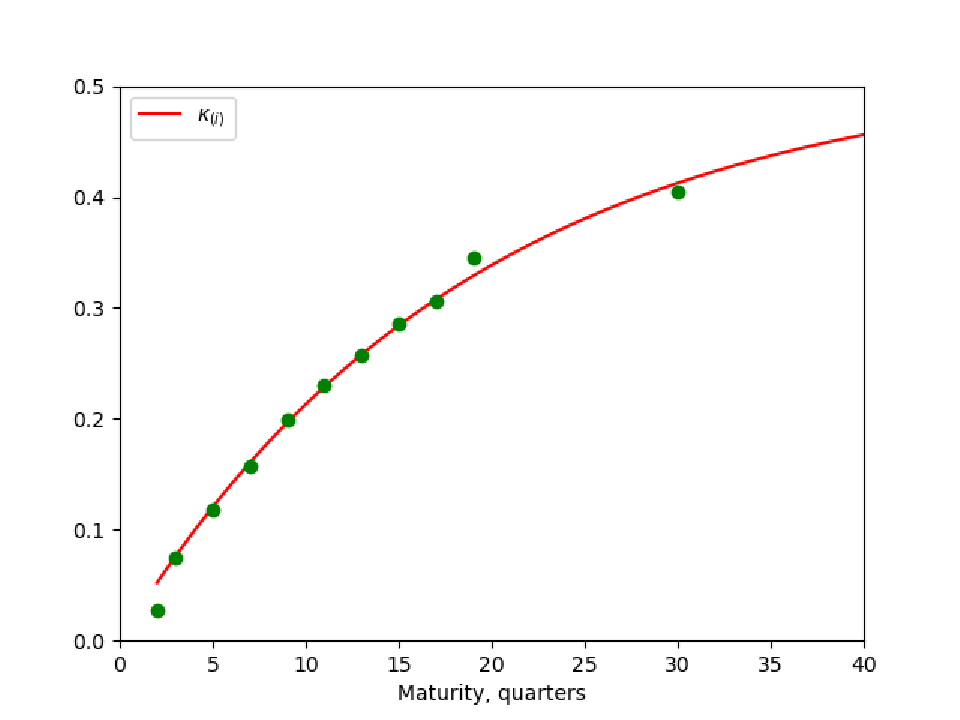
\includegraphics[width=0.4\paperwidth]{figdata/fit_kappa}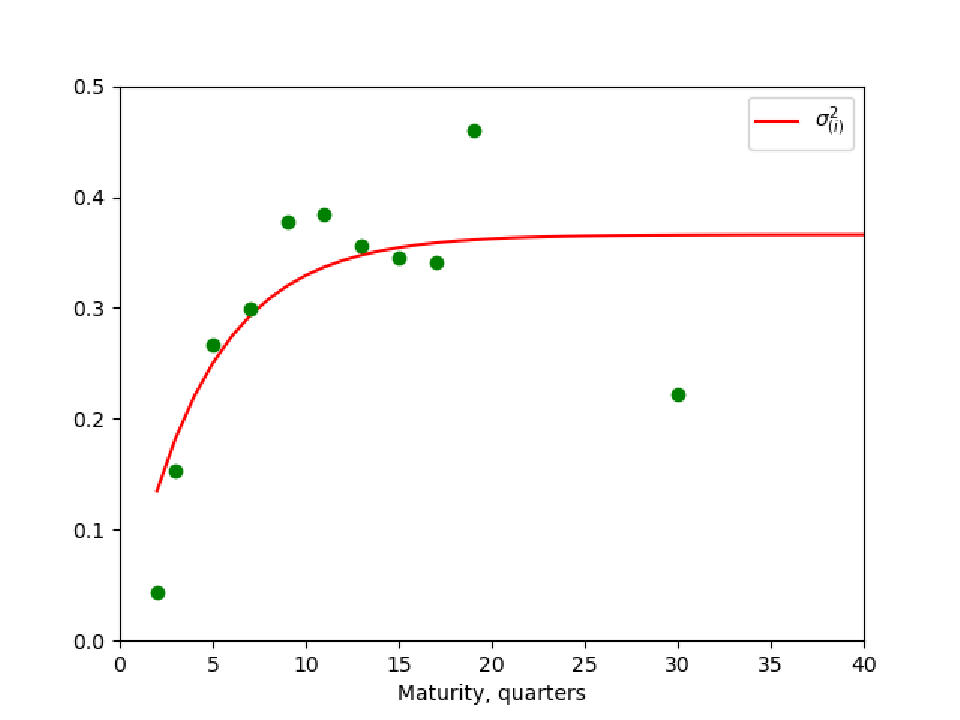
\includegraphics[width=0.4\paperwidth]{figdata/fit_sigma}\caption{Fit for extrapolation of the factor model estimates of $\left(\kappa_{j},\sigma_{j}^{2}\right)$
using $f(j)=e^{0}-e^{0}\exp(-e^{1}\times j)$ for factor model \eqref{eq: factor model}.
The dotted points are the point estimates and the bold line is the
interpolation.}
\par\end{centering}
\centering{}\caption{\label{fig:Interpolated-and-extrapolated_infinite maturities}}
\end{figure}


\paragraph*{Fit of covariances}

In the text we mention that a test for the factor model is how well
it captures contemporaneous covariances. To implement this test we
compute $cov(r^{j},G)$ and $cov(r^{j},\Theta)$ using the estimated
factor model and plot it against the ones computed using the raw data
for the 11 portfolios that we use. In Figure \ref{fig: cov fit},
we see the fit is good. 
\begin{figure}
\centering{}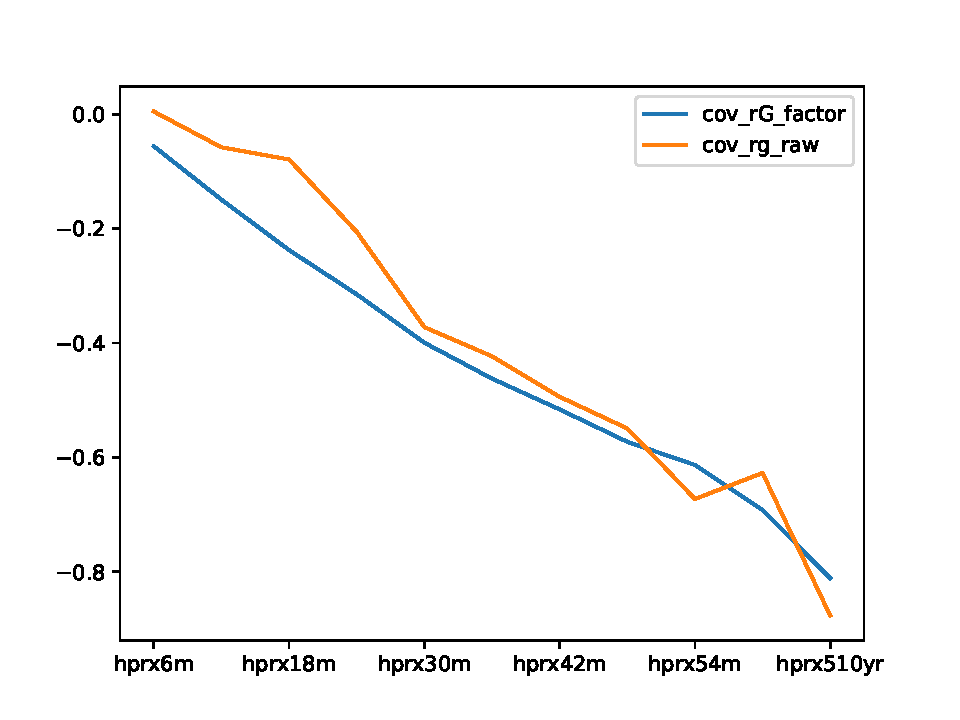
\includegraphics[width=0.4\paperwidth]{figdata/cov_rG}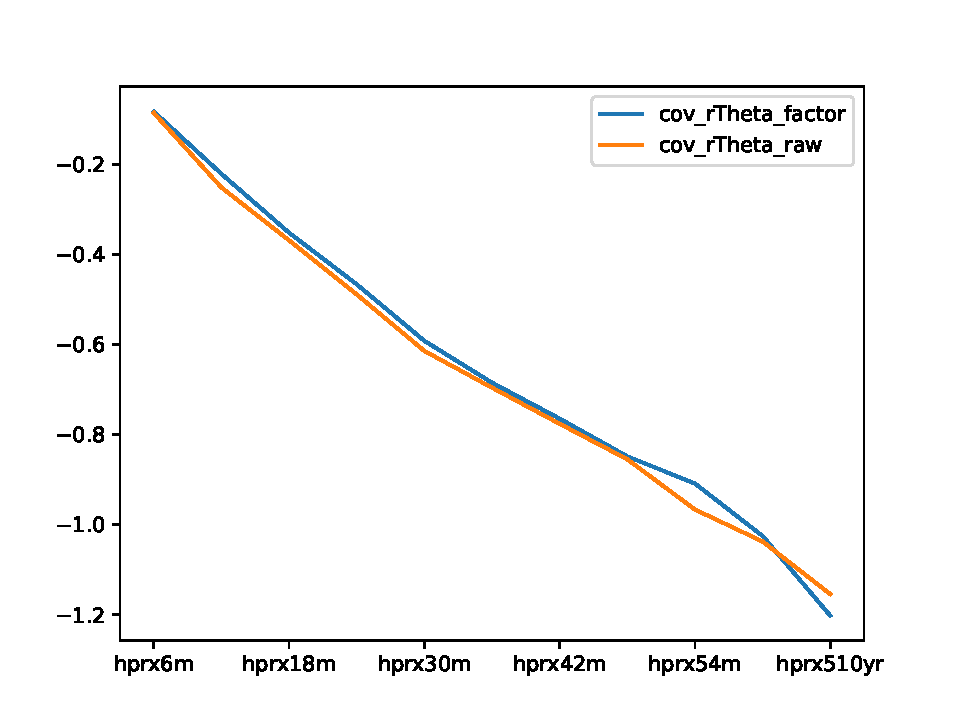
\includegraphics[width=0.4\paperwidth]{figdata/cov_rTheta}\caption{\label{fig: cov fit} Fit for contemporaneous covariances. The blue
lines is computed using the estimates of the factor model and the
orange line is computed using the data for the sample period 1952-2017.}
\end{figure}


\paragraph*{Components of the target portfolio}

In Figure \ref{fig: components g, Theta, Q}, we breakup the target
portfolio into the portfolio that hedges government spending $\omega_{t}^{G}$,
tax revenue risk $\omega_{t}^{\Theta}$, and interest rate risk $\omega_{t}^{Q}$.

\begin{figure}
\centering{}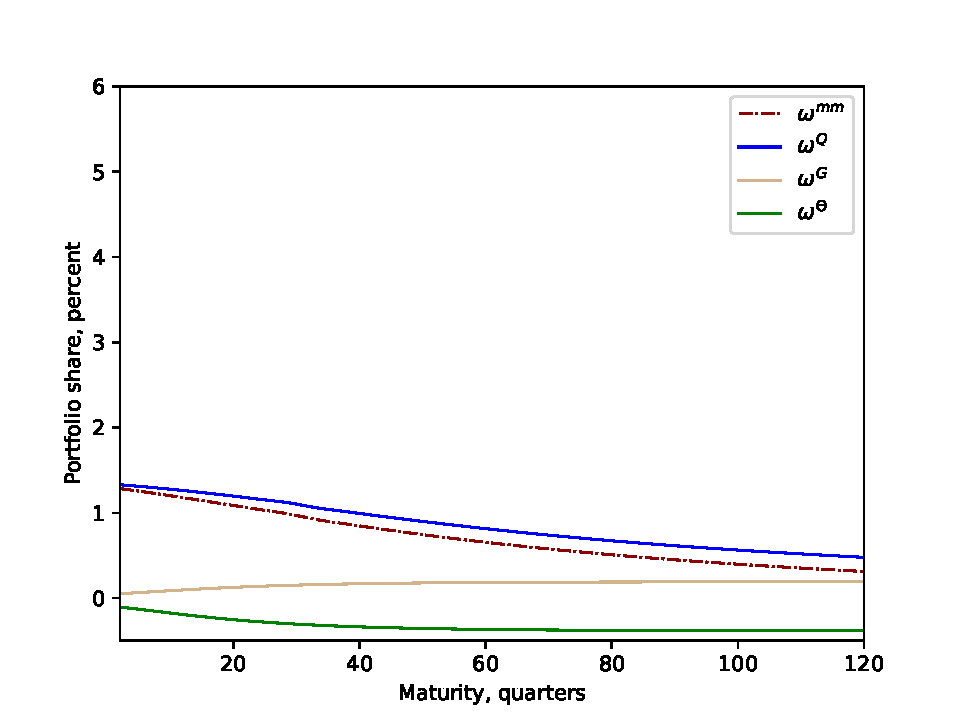
\includegraphics[width=0.5\paperwidth]{figdata/3comps}\caption{\label{fig: components g, Theta, Q} Components of the target portfolio.}
\end{figure}


\subsection{Robustness \label{sec: App_ Robustness baseline}}

\paragraph*{Factor-mimicking portfolios}

In the main text, our factor model was based on principal components
extracted from returns and macroeconomic data. There is a tradition
in the finance literature to use factor-mimicking portfolios. These
portfolios are constructed be projecting macro variables on a set
of returns and using the projection coefficients to construct portfolios.
Practitioners then replace the poorly-measured macro variables with
returns on those constructed portfolios. In our context extracting
principal components from returns and projections on returns is the
same as extracting them from only return data. In Figure \ref{fig: factor mimicking},
we report results using the common factor using only bond return data.

\begin{figure}
	\begin{centering}
		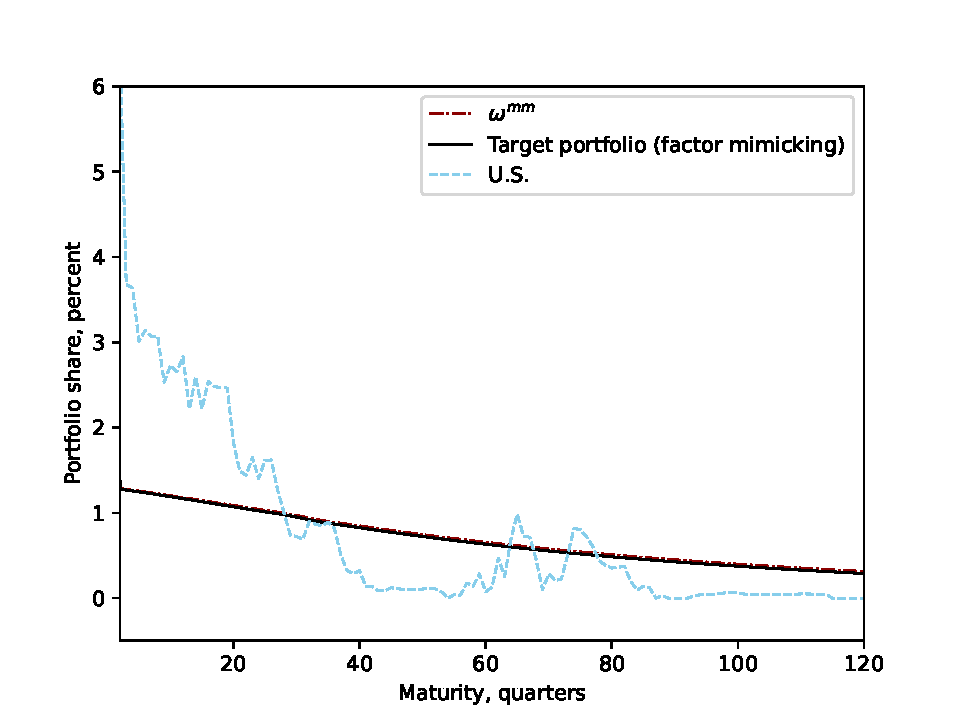
\includegraphics[width=0.4\paperwidth]{figdata/opt_us_factor_mm}
		\caption{Target portfolio using the common factor extracted from bond excess returns.}
	\end{centering}
	\caption{\label{fig: factor mimicking}}
\end{figure}
	

\paragraph{Multifactor}

We extend the factor model to have multiple factors. Let $z_{t}$
be a stacked vector that consists of excess returns $\left\{ r_{t}^{j}\right\} _{j}$
for the 11 portfolios of different maturities $j$, a measure of $\ln\Theta_{t}$
and expenditures $\ln G_{t}$. We use $z_{t}^{k}$ to denote the $k^{th}$
element of this vector. We posit the following stochastic process
\begin{align}
z_{t}^{k} & =\alpha_{k}+\rho_{k}z_{t-1}^{k}+\sum_{m}\kappa_{m,k}f_{t}^{m}+\varepsilon_{t}^{k}\text{ for all }k,\nonumber \\
f_{t}^{n} & =\alpha_{f}^{n}+\sum_{m}\kappa_{m,f}f_{t}^{m}+\varepsilon_{t}^{f,n}\text{ for all }j=1\dots n,\label{eq: factor model-1}
\end{align}
where $\text{\ensuremath{\left\{  f_{t}^{n}\right\} } }_{n}$ are
a set of factors and $\left\{ \varepsilon_{t}^{k},\varepsilon_{t}^{f,n}\right\} _{k,t}$
are residuals. We use the subscripts $k\in\left\{ \Theta,G\right\} $
to denote the variables $\ln\Theta_{t}$, $\ln G_{t}$, and $k=j$
to denote returns on bonds of maturity $j$. In this section, we report
the estimates of the factor model and other details skipped in the
main text.

With multiple factors the covariance of returns with each other is
given by $\Sigma_{t}=\Delta+\kappa\Delta_{f}\kappa^{\intercal}$ where
$\Delta=diag\text{\ensuremath{\left\{  \sigma_{j}^{2}\right\} } },$$\kappa=\left[\kappa_{1}\quad\kappa_{2}\ldots\right]$
is the matrix of factor loadings on returns and inverse $\Sigma_{t}^{-1}$
can be obtained using Woodbury matrix identity. As before, we use
Lemma \ref{lem: key asset pricing fact} to compute $\Sigma_{t}^{Q}$
using $\Sigma_{t}.$ The covariances with spending and tax revenue
risk are given by $\Sigma_{t}^{G}[j]=\sum_{n}\kappa_{n,j}\kappa_{n,G}\sigma_{f^{n}}^{2}$
and $\Sigma_{t}^{\Theta}[j]=\sum_{n}\kappa_{n,j}\kappa_{n,\Theta}\sigma_{f^{n}}^{2}$.
The weights $\left\{ s_{t}^{Q},s_{t}^{G},s_{t}^{\Theta}\right\} _{t}$
are unchanged.

In Figure \ref{fig: 2 factors}, we plot the first two principal components
extracted from excess returns, the risk-free rate, GDP (detrended),
deficits/GDP. We see that the second factor is less volatile relative
to the first factor. We next report the factor loadings for the two
factor model in Table \ref{tab: Factor model estimation MF}.

\begin{figure}
\begin{tikzpicture}
\def\myplotFILENAME{figdata/factordata.csv}
\pgfplotstableread[col sep=comma]{\myplotFILENAME}\myplotDataFactor

\begin{axis}[     title={Factor},     xlabel={Date},     height=0.25\textheight,width=\textwidth,scaled x ticks = false,   x tick label style={/pgf/number format/.cd, 1000 sep={}}, xmin=1950,xmax=2016, xtick={1950,1980,...,2017},legend pos=north east,       y tick label style={/pgf/number format/.cd,           scaled y ticks = false,           set thousands separator={},           fixed}] 

% Here we plot the data from the CSV file 

\addplot[line width=1.5pt,color=black]  table[x=datealt, y=factor1] {\myplotDataFactor}; 
\addlegendentry{$1^{st}$ Factor}
\addplot[line width=1.5pt,color=orange]  table[x=datealt, y=factor2] {\myplotDataFactor}; 
\addlegendentry{$2^{nd}$ Factor}
\end{axis} 
\end{tikzpicture} \caption{Time series for the first two principal components \label{fig: 2 factors}}
\end{figure}

\begin{table}
\begin{centering}
\caption{FACTOR LOADINGS (MULTIFACTOR)\label{tab: Factor model estimation MF}}
\medskip{}
 \medskip{}
 %
\begin{tabular}{>{\raggedright}p{0.68cm}>{\centering}p{0.68cm}>{\raggedright}p{0.68cm}>{\raggedright}p{0.68cm}>{\raggedright}p{0.68cm}>{\raggedright}p{0.68cm}>{\raggedright}p{0.68cm}>{\raggedright}p{0.68cm}>{\raggedright}p{0.68cm}>{\raggedright}p{0.68cm}>{\raggedright}p{0.68cm}>{\raggedright}p{0.68cm}>{\raggedright}p{0.68cm}>{\raggedright}p{0.68cm}>{\raggedright}p{0.68cm}}
\hline 
\raggedright{} & \multicolumn{11}{c}{{\tiny{}{}Excess returns $r_{t}^{j}$ for various maturities $j$}} & \multicolumn{3}{l}{}\tabularnewline
\hline 
\raggedright{} & \raggedright{}{\tiny{}{}6m} & \raggedright{}{\tiny{}{}12m} & \raggedright{}{\tiny{}{}18m} & \raggedright{}{\tiny{}{}24m} & \raggedright{}{\tiny{}{}30m} & \raggedright{}{\tiny{}{}36m} & \raggedright{}{\tiny{}{}42m} & \raggedright{}{\tiny{}{}48m} & \raggedright{}{\tiny{}{}54m} & \raggedright{}{\tiny{}{}60m} & \raggedright{}{\tiny{}{}120m} & \raggedright{}{\tiny{}{}$\ln G_{t}$} & \raggedright{}{\tiny{}{}$\ln\Theta_{t}$} & \raggedright{}{\tiny{}{}}\tabularnewline
{\tiny{}$\kappa_{1,k}$} & {\tiny{}0.028} & {\tiny{}0.075} & {\tiny{}0.119} & {\tiny{}0.157} & {\tiny{}0.200} & {\tiny{}0.231} & {\tiny{}0.257} & {\tiny{}0.286} & {\tiny{}0.306} & {\tiny{}0.345} & {\tiny{}0.404} & {\tiny{}-0.032} & {\tiny{}-0.047} & \tabularnewline
{\tiny{}s.e} & {\tiny{}0.001} & {\tiny{}0.002} & {\tiny{}0.002} & {\tiny{}0.002} & {\tiny{}0.002} & {\tiny{}0.002} & {\tiny{}0.002} & {\tiny{}0.003} & {\tiny{}0.003} & {\tiny{}0.004} & {\tiny{}0.004} & {\tiny{}0.016} & {\tiny{}0.008} & \tabularnewline
{\tiny{}$\kappa_{2,k}$} & {\tiny{}-0.053} & {\tiny{}-0.126} & {\tiny{}-0.183} & {\tiny{}-0.208} & {\tiny{}-0.244} & {\tiny{}-0.248} & {\tiny{}-0.248} & {\tiny{}-0.218} & {\tiny{}-0.198} & {\tiny{}-0.184} & {\tiny{}-0.066} & {\tiny{}-0.031} & {\tiny{}0.024} & \tabularnewline
{\tiny{}s.e} & {\tiny{}0.005} & {\tiny{}0.008} & {\tiny{}0.009} & {\tiny{}0.008} & {\tiny{}0.008} & {\tiny{}0.008} & {\tiny{}0.006} & {\tiny{}0.009} & {\tiny{}0.011} & {\tiny{}0.015} & {\tiny{}0.013} & {\tiny{}0.058} & {\tiny{}0.030} & \tabularnewline
{\tiny{}$\sigma_{k}^{2}$} & {\tiny{}0.030} & {\tiny{}0.074} & {\tiny{}0.098} & {\tiny{}0.083} & {\tiny{}0.082} & {\tiny{}0.077} & {\tiny{}0.048} & {\tiny{}0.107} & {\tiny{}0.145} & {\tiny{}0.292} & {\tiny{}0.200} & {\tiny{}4.227} & {\tiny{}1.143} & \tabularnewline
{\tiny{}s.e} & {\tiny{}0.003} & {\tiny{}0.007} & {\tiny{}0.009} & {\tiny{}0.007} & {\tiny{}0.007} & {\tiny{}0.007} & {\tiny{}0.004} & {\tiny{}0.009} & {\tiny{}0.013} & {\tiny{}0.026} & {\tiny{}0.018} & {\tiny{}0.374} & {\tiny{}0.101} & \tabularnewline
\hline 
{\tiny{}$R^{2}$} & {\tiny{}0.536} & {\tiny{}0.698} & {\tiny{}0.771} & {\tiny{}0.840} & {\tiny{}0.870} & {\tiny{}0.898} & {\tiny{}0.922} & {\tiny{}0.938} & {\tiny{}0.946} & {\tiny{}0.943} & {\tiny{}0.979} & {\tiny{}0.016} & {\tiny{}0.111} & \tabularnewline
\end{tabular}
\par\end{centering}
\noindent %
\noindent\begin{minipage}[t]{1\columnwidth}%
{\footnotesize{}{}{}{}{}{}{}}{\scriptsize{}{}Notes: This table
records the OLS factor loadings for the two factor version of the
model (\ref{eq: factor model}). Standards errors are in parenthesis.The
row titled ``R2'' are values of R-squared for each equation in the
system (\ref{eq: factor model}). The sample for excess returns and
primary surpluses normalized by outputs is 1952-2017, and the sample
for the one-period liquidity premium is 1984-2017. The time period
is a quarter.}%
\end{minipage}
\end{table}


\subparagraph*{Fit of covariances}

Figure \ref{fig: cov fit mf} plots the counterpart of Figure \ref{fig: cov fit}
for the multifactor model. We see that the fit is similar and slightly
better than the single factor model.

\begin{figure}
\centering{}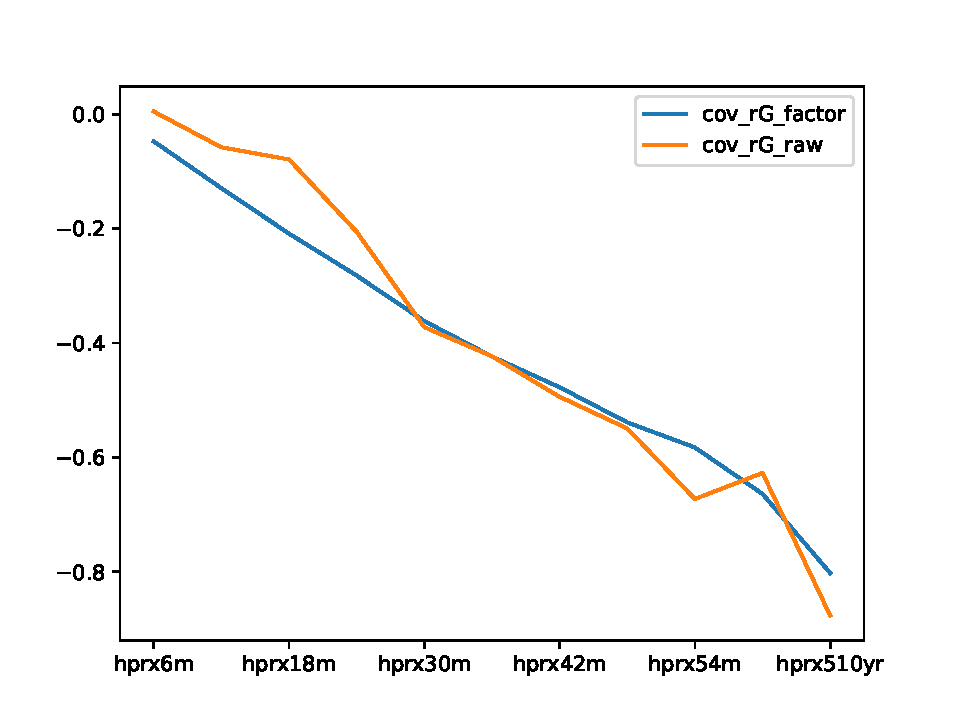
\includegraphics[width=0.4\paperwidth]{figdata/cov_rG_MF}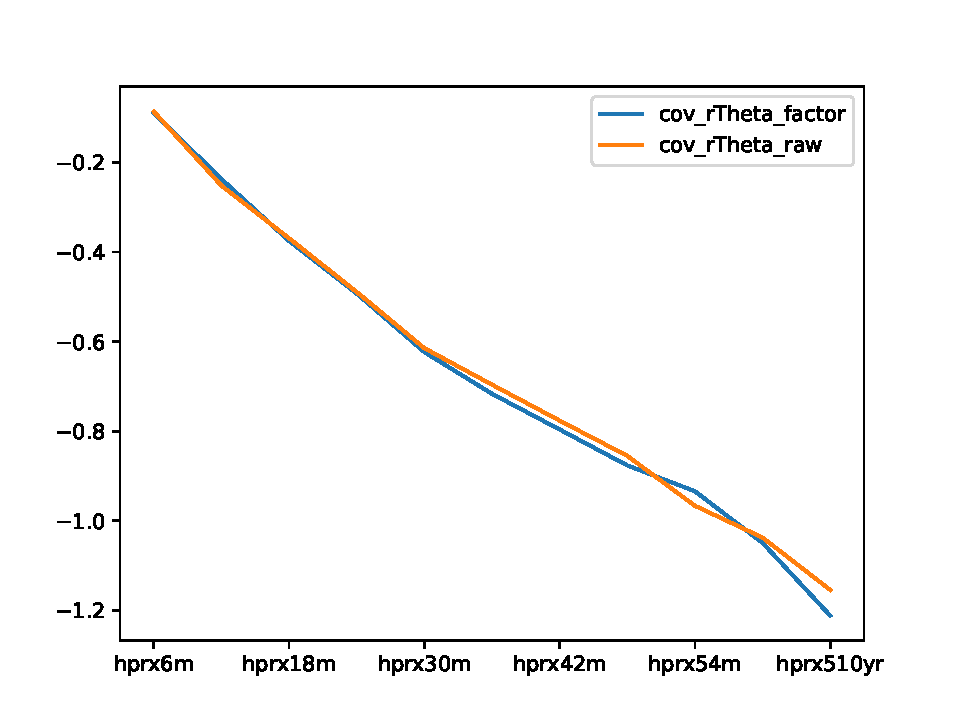
\includegraphics[width=0.4\paperwidth]{figdata/cov_rTheta_MF}\caption{\label{fig: cov fit mf} Fit for contemporaneous covariances. The
blue lines is computed using the estimates of the multi-factor version
of the factor model and the orange line is computed using the data
for the sample period 1952-2017.}
\end{figure}


\subparagraph*{Extrapolation of loadings}

In Figure \ref{fig:Interpolated-and-extrapolated_infinite maturities 2 factor},
we plot the fit for the factor loadings for the multifactor model.
We use the same form for the first factor as the baseline in the text.
The second factor is non-monotonic and has a hump shape for intermediate
maturities. To capture that hump, we use the functional form $e^{0}+e^{1}\text{exp}(-(j-e^{2})^{2}/e^{3})$.
We see in Figure \ref{fig:Interpolated-and-extrapolated_infinite maturities 2 factor}
that the interpolated lines fit well the point estimates.

\begin{figure}
\centering{}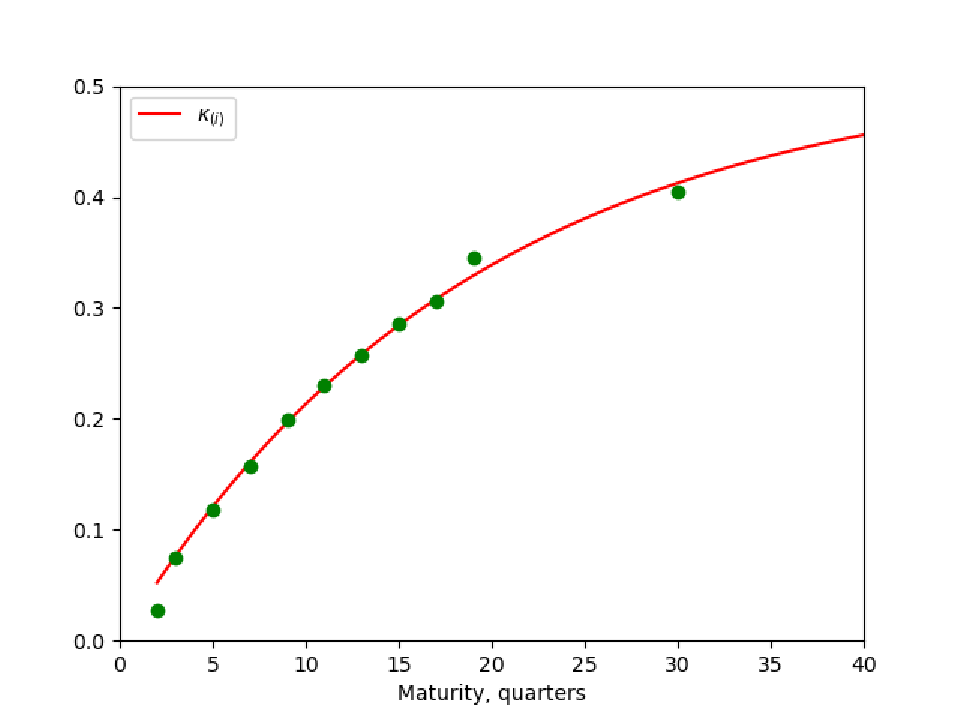
\includegraphics[width=0.4\paperwidth]{figdata/fit_kappa_2fac_1}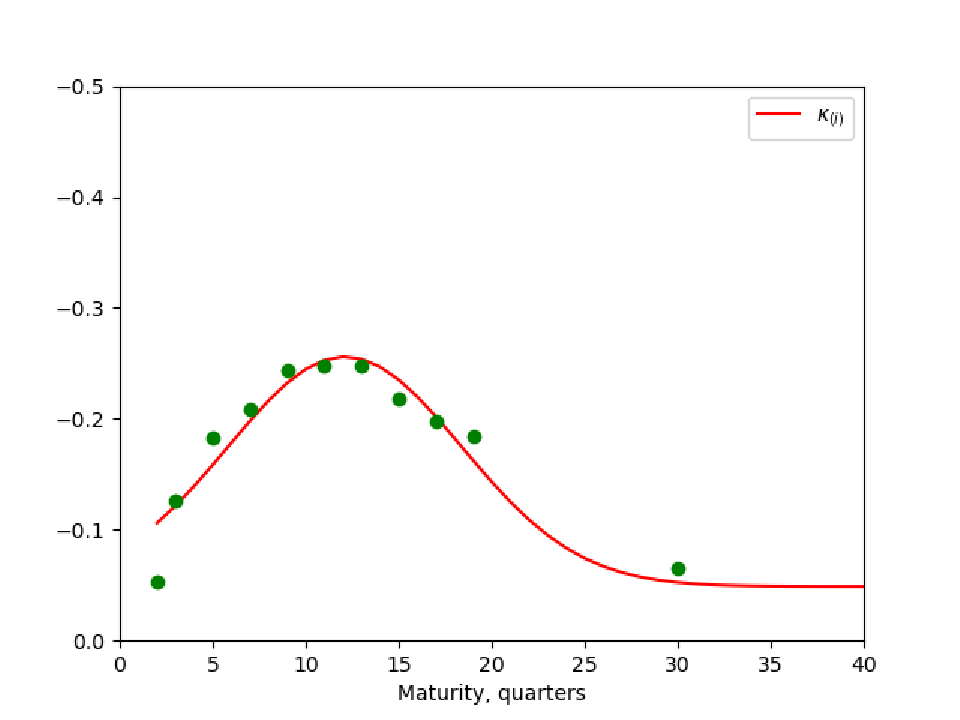
\includegraphics[width=0.4\paperwidth]{figdata/fit_kappa_2fac_2}\caption{\label{fig:Interpolated-and-extrapolated_infinite maturities 2 factor}
Fit for extrapolation of multifactor model estimates of $\left(\kappa_{1,j},\kappa_{2,j}\right)$.
For the first factor, we use the functional form $f(j)=e^{0}-e^{0}\exp(-e^{1}\times j)$
and for the second factor we use the functional form $(e^{0}+e^{1}\text{exp}(-(j-e^{2})^{2}/e^{3}))$.
The dotted points are the point estimates and the bold line is the
interpolation.}
\end{figure}


\paragraph{Limiting Portfolio with One Factor}

In the main text, we compared the limiting portfolio as we send the
estimated $\sigma_{j}^{2}\to0$ for each $j$ and keep the factor
loadings $\left\{ \kappa_{n,j}\right\} _{n,j}$ for the multifactor
setting. In Figure (\ref{limiting portfolio one factor}), we plot
the corresponding figure for the baseline target portfolio with one
factor.

\begin{figure}
\begin{centering}
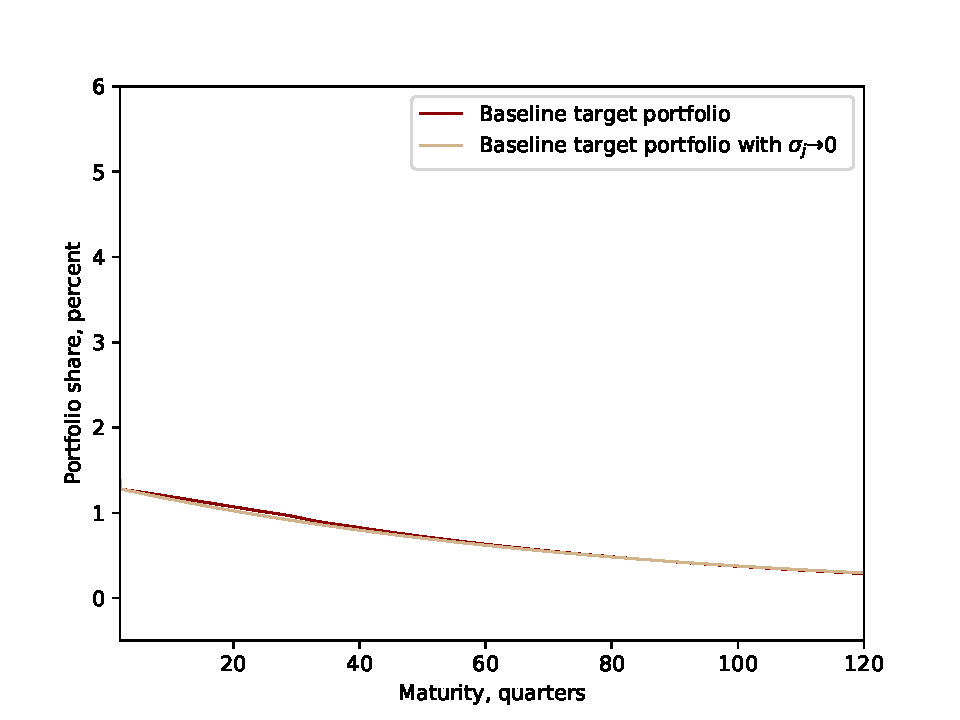
\includegraphics[width=0.5\paperwidth]{figdata/noise_1F}
\par\end{centering}
\caption{\label{limiting portfolio one factor} Comparison of the baseline
target portfolio to the limiting portfolio in which we set $\sigma_{j}^{2}\to0$
for each $j$.}
\end{figure}


\paragraph*{AR(1) factor structure}

We consider the general estimation of (\ref{eq: factor model}) without
any a-priori restrictions on parameters. Table \ref{Factor model estimation-AR1-1}
presents estimation results. We see from the table that we cannot
reject $\rho_{G}=\rho_{\Theta}=1$ and $\rho_{f}=0.$
\begin{table}
\begin{centering}
\caption{FACTOR MODEL ESTIMATION RESULTS (AR(1) FACTOR STRUCTURE)\label{Factor model estimation-AR1-1}}
\medskip{}
\medskip{}
\begin{tabular}{>{\raggedright}p{0.68cm}>{\centering}p{0.68cm}>{\raggedright}p{0.68cm}>{\raggedright}p{0.68cm}>{\raggedright}p{0.68cm}>{\raggedright}p{0.68cm}>{\raggedright}p{0.68cm}>{\raggedright}p{0.68cm}>{\raggedright}p{0.68cm}>{\raggedright}p{0.68cm}>{\raggedright}p{0.68cm}>{\raggedright}p{0.68cm}>{\raggedright}p{0.68cm}>{\raggedright}p{0.68cm}>{\raggedright}p{0.68cm}}
\hline 
\raggedright{} & \multicolumn{11}{c}{{\tiny{}Excess returns $r_{t}^{j}$ for various maturities $j$}} & \multicolumn{3}{l}{}\tabularnewline
\hline 
\raggedright{} & \raggedright{}{\tiny{}6m} & \raggedright{}{\tiny{}12m} & \raggedright{}{\tiny{}18m} & \raggedright{}{\tiny{}24m} & \raggedright{}{\tiny{}30m} & \raggedright{}{\tiny{}36m} & \raggedright{}{\tiny{}42m} & \raggedright{}{\tiny{}48m} & \raggedright{}{\tiny{}54m} & \raggedright{}{\tiny{}60m} & \raggedright{}{\tiny{}120m} & \raggedright{}{\tiny{}$\ln G_{t}$} & \raggedright{}{\tiny{}$\ln\Theta_{t}$} & \raggedright{}{\tiny{}$f_{t}$}\tabularnewline
\raggedright{}{\scriptsize{}$\alpha_{k}$} & {\tiny{}0.086} & {\tiny{}0.155} & {\tiny{}0.220} & {\tiny{}0.245} & {\tiny{}0.284} & {\tiny{}0.315} & {\tiny{}0.346} & {\tiny{}0.344} & {\tiny{}0.372} & {\tiny{}0.304} & {\tiny{}0.444} & {\tiny{}-0.177} & {\tiny{}-0.319} & {\tiny{}0.026}\tabularnewline
\raggedright{} & \raggedright{}{\tiny{}\vspace{-6mm}(0.014)} & \raggedright{}{\tiny{}\vspace{-6mm}(0.025)} & \raggedright{}{\tiny{}\vspace{-6mm}(0.033)} & \raggedright{}{\tiny{}\vspace{-6mm}(0.035)} & \raggedright{}{\tiny{}\vspace{-6mm}(0.039)} & \raggedright{}{\tiny{}\vspace{-6mm}(0.039)} & \raggedright{}{\tiny{}\vspace{-6mm}(0.038)} & \raggedright{}{\tiny{}\vspace{-6mm}(0.037)} & \raggedright{}{\tiny{}\vspace{-6mm}(0.037)} & \raggedright{}{\tiny{}\vspace{-6mm}(0.043)} & \raggedright{}{\tiny{}\vspace{-6mm}(0.030)} & \raggedright{}{\tiny{}\vspace{-6mm}(0.016)} & \raggedright{}{\tiny{}\vspace{-6mm}(0.008)} & \raggedright{}{\tiny{}\vspace{-6mm}(0.502)}\tabularnewline
\raggedright{}{\scriptsize{}$\rho_{k}$} & {\tiny{}-0.107} & {\tiny{}-0.057} & {\tiny{}-0.041} & {\tiny{}-0.043} & {\tiny{}-0.042} & {\tiny{}-0.025} & {\tiny{}-0.022} & {\tiny{}-0.008} & {\tiny{}-0.022} & {\tiny{}-0.027} & {\tiny{}0.003} & {\tiny{}1.001} & {\tiny{}1.009} & {\tiny{}-0.035}\tabularnewline
\raggedright{} & \raggedright{}{\tiny{}\vspace{-6mm}(0.043)} & \raggedright{}{\tiny{}\vspace{-6mm}(0.035)} & \raggedright{}{\tiny{}\vspace{-6mm}(0.030)} & \raggedright{}{\tiny{}\vspace{-6mm}(0.025)} & \raggedright{}{\tiny{}\vspace{-6mm}(0.023)} & \raggedright{}{\tiny{}\vspace{-6mm}(0.020)} & \raggedright{}{\tiny{}\vspace{-6mm}(0.018)} & \raggedright{}{\tiny{}\vspace{-6mm}(0.016)} & \raggedright{}{\tiny{}\vspace{-6mm}(0.015)} & \raggedright{}{\tiny{}\vspace{-6mm}(0.015)} & \raggedright{}{\tiny{}\vspace{-6mm}(0.009)} & \raggedright{}{\tiny{}\vspace{-6mm}(0.008)} & \raggedright{}{\tiny{}\vspace{-6mm}(0.004)} & \raggedright{}{\tiny{}\vspace{-6mm}(0.063)}\tabularnewline
\raggedright{}{\scriptsize{}$\kappa_{k}$} & {\tiny{}0.028} & {\tiny{}0.074} & {\tiny{}0.118} & {\tiny{}0.157} & {\tiny{}0.199} & {\tiny{}0.230} & {\tiny{}0.257} & {\tiny{}0.285} & {\tiny{}0.306} & {\tiny{}0.345} & {\tiny{}0.404} & {\tiny{}-0.032} & {\tiny{}-0.048} & {\tiny{}0.000}\tabularnewline
\raggedright{} & \raggedright{}{\tiny{}\vspace{-6mm}(0.002)} & \raggedright{}{\tiny{}\vspace{-6mm}(0.003)} & \raggedright{}{\tiny{}\vspace{-6mm}(0.004)} & \raggedright{}{\tiny{}\vspace{-6mm}(0.004)} & \raggedright{}{\tiny{}\vspace{-6mm}(0.005)} & \raggedright{}{\tiny{}\vspace{-6mm}(0.005)} & \raggedright{}{\tiny{}\vspace{-6mm}(0.005)} & \raggedright{}{\tiny{}\vspace{-6mm}(0.005)} & \raggedright{}{\tiny{}\vspace{-6mm}(0.005)} & \raggedright{}{\tiny{}\vspace{-6mm}(0.005)} & \raggedright{}{\tiny{}\vspace{-6mm}(0.004)} & \raggedright{}{\tiny{}\vspace{-6mm}(0.016)} & \raggedright{}{\tiny{}\vspace{-6mm}(0.008)} & \raggedright{}{\tiny{}\vspace{-6mm}(nan)}\tabularnewline
\raggedright{}{\scriptsize{}$\sigma_{k}^{2}$} & {\tiny{}0.044} & {\tiny{}0.154} & {\tiny{}0.267} & {\tiny{}0.300} & {\tiny{}0.378} & {\tiny{}0.384} & {\tiny{}0.356} & {\tiny{}0.345} & {\tiny{}0.341} & {\tiny{}0.460} & {\tiny{}0.222} & {\tiny{}4.231} & {\tiny{}1.125} & {\tiny{}63.676}\tabularnewline
\raggedright{} & \raggedright{}{\tiny{}\vspace{-6mm}(0.004)} & \raggedright{}{\tiny{}\vspace{-6mm}(0.014)} & \raggedright{}{\tiny{}\vspace{-6mm}(0.024)} & \raggedright{}{\tiny{}\vspace{-6mm}(0.027)} & \raggedright{}{\tiny{}\vspace{-6mm}(0.034)} & \raggedright{}{\tiny{}\vspace{-6mm}(0.034)} & \raggedright{}{\tiny{}\vspace{-6mm}(0.031)} & \raggedright{}{\tiny{}\vspace{-6mm}(0.031)} & \raggedright{}{\tiny{}\vspace{-6mm}(0.030)} & \raggedright{}{\tiny{}\vspace{-6mm}(0.041)} & \raggedright{}{\tiny{}\vspace{-6mm}(0.020)} & \raggedright{}{\tiny{}\vspace{-6mm}(0.375)} & \raggedright{}{\tiny{}\vspace{-6mm}(0.100)} & \raggedright{}{\tiny{}\vspace{-6mm}(5.65)}\tabularnewline
\hline 
\raggedright{}{\scriptsize{}R2} & {\tiny{}0.536} & {\tiny{}0.698} & {\tiny{}0.771} & {\tiny{}0.840} & {\tiny{}0.870} & {\tiny{}0.898} & {\tiny{}0.922} & {\tiny{}0.938} & {\tiny{}0.946} & {\tiny{}0.943} & {\tiny{}0.979} & {\tiny{}0.985} & {\tiny{}0.996} & {\tiny{}0.001}\tabularnewline
\end{tabular}
\par\end{centering}
\noindent\begin{minipage}[t]{1\columnwidth}%
{\footnotesize{}{}{}{}{}{}}{\scriptsize{}Notes: This table records
the OLS estimates of the factor model (\ref{eq: factor model}) without
imposing $\rho_{f}=0,\rho_{\Theta}=\rho_{G}=1$. Standards errors
are in parenthesis. The sample for excess returns and primary surpluses
normalized by outputs is 1952-2017. The time period is a quarter.}%
\end{minipage}
\end{table}


\paragraph{Transitory Shock}

We assume that the spending is given by $G_{t}=G_{t}^{p}G_{t}^{tr}$
with $G_{t}^{p}$ following the same structure as the baseline (\ref{eq: factor model})
and $G_{t}^{tr}=\rho_{tr}G_{t-1}^{tr}$. We then simulate the target
portfolio for alternative values of the transitory $\left\{ G_{t}^{tr},\rho_{tr}\right\} $.

Such a shock affects the path of spending, the optimal tax rate, and
through the optimal tax rate the expected path of tax revenues. The
tax revenue risk weights are unchanged but the weights on spending
risk $s_{t}^{G}[k]=\frac{-Q_{t}^{k}\left(\Gamma\right)^{k}G_{t}\left(G_{t}^{tr}\right)^{1-\rho_{tr}^{k}}}{Q_{t}^{1}B_{t}}$
and the weights on interest rate risk $s_{t}^{Q}[k]=\frac{Q_{t}^{k+1}\left(\Gamma\right)^{k+1}\left(T_{t}^{tax}-G_{t}\left(G_{T}^{tr}\right)^{1-\rho_{tr}^{k+1}}\right)}{Q_{t}^{1}\sum Q_{t}^{k+1}\left(\Gamma\right)^{k+1}\left(T_{t}^{tax}-G_{t}\left(G_{t}^{tr}\right)^{1-\rho_{tr}^{k+1}}\right)}$
where $T_{t}^{tax}$ are the tax revenues computed at the optimal
tax rate that is constant and balances the inter temporal budget at
the zeroth order given the path of spending.

In left panel Figure \ref{fig:predictability}, we show the target
portfolio setting for a 10\% and 20\% increase in the share of spending
to GDP with $\rho_{tr}=0.75$ so that the increase lasts for about
5 years. In right panel, we plot the target portfolios for the same
values of $G_{t}^{tr}$ but a higher value of $\rho_{tr}=.95$.

\begin{figure}
\begin{centering}
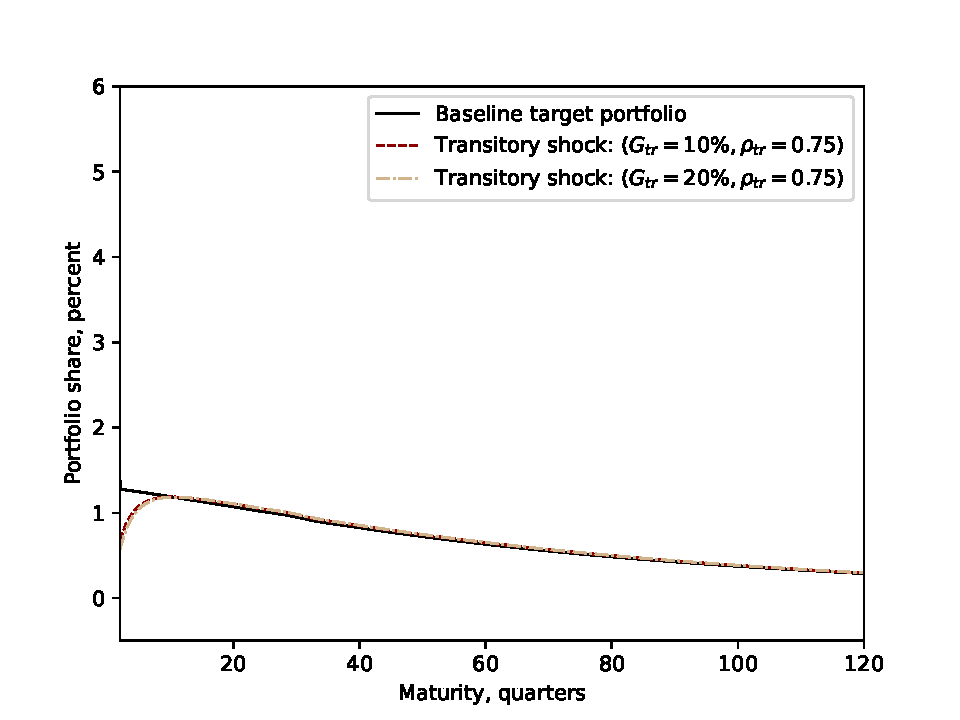
\includegraphics[width=0.4\paperwidth]{figdata/opt_gtr75}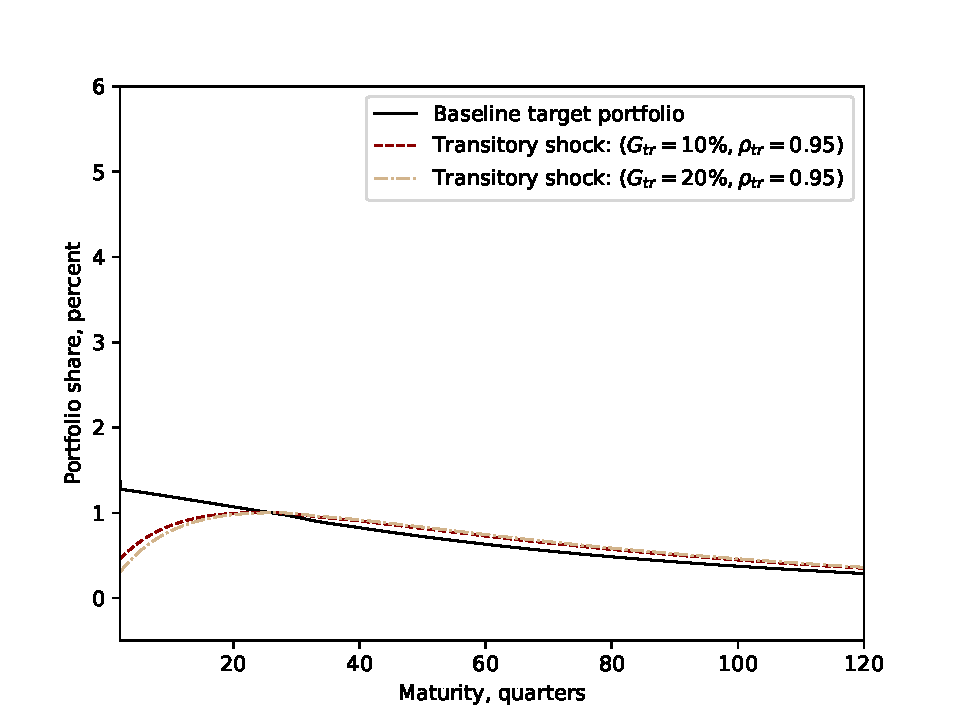
\includegraphics[width=0.4\paperwidth]{figdata/opt_gtr95}
\par\end{centering}
\caption{Comparison of optimal portfolios with a transitory increase in spending.
In left panel we show the target portfolio for $\ln G_{t}^{tr}\in\left\{ 10\%,20\%\right\} $
with $\rho_{tr}=0.75$ and i n right panel, we plot the target portfolios
for for $\ln G_{t}^{tr}\in\left\{ 10\%,20\%\right\} $ with $\rho_{tr}=0.95$
. \label{fig:predictability}}
\end{figure}


\paragraph{Heteroskedastic shocks \label{subsec:Heteroskedastic-shocks}}

In the main text, we assumed that the shocks $\mathbf{\varepsilon}_{t}$
were homoskedastic, that is, we imposed that $\left\{ \sigma_{k}\right\} $
for $k\in$$\left\{ j,Y,G,A,f\right\} $ are constant through time.
We relax that assumption and augment the baseline factor model \eqref{eq: factor model}
with the following univariate GARH processes $\left\{ \sigma_{k}\right\} $
\[
\sigma_{k,t}^{2}=\overline{\sigma}_{k}^{2}+\sum_{j=1}^{p}\rho_{kp}^{GARCH}\varepsilon_{zt-p}^{2}+\sum_{j=1}^{q}\varrho_{kq}^{GARCH}\sigma_{\varepsilon z,t-q}^{2}
\]
and impose that all $\varepsilon$ are standard Gaussian and independent
of each other. We now estimate the system using maximum likelihood
and assuming $p=2$ and $q=1$.

The consequence of heteroskedastic shocks is that structure of the
expressions for $\Sigma_{T}$ and $\Sigma_{T}^{-1}$ as well as $\Sigma_{T}^{k}$for
$k\in\left\{ X,A,Q\right\} $ remains the same but they have time-varying
parameters $\sigma_{f,t}$ and $\sigma_{j,t}$ for each return maturities
$j$.\footnote{The time-variation in $\left\{ \sigma_{G}^{2},\sigma_{Y}^{2},\sigma_{A}^{2}\right\} $
drops out because the covariances of hedging terms are driven by the
common component captured in the factor $\left\{ \sigma_{f,t}^{2}\right\} .$} We use the same extrapolation scheme as the baseline to obtain $\left(\sigma_{j},\kappa_{j}\right)$
for other maturities. And finally, as an implication, the optimal
target portfolio and its components also inherit that time-variation.\footnote{In principle, the fiscal risk and liquidity risk portfolio could vary
because quasi-weights $\pi_{T}^{X}$ and $\pi_{T}^{A}$ or $\vec{\beta}$
vary with time. To focus on the impact of heteroskedastic shocks,
we keep them constant and equal to the values that we used in the
main text and only allow the target portfolio to vary due to time-varying
covariances.}

In Figure \ref{vol}, we plot the time-series for elements in $\left\{ \sigma_{j,t}\right\} $
and $\sigma_{f,t}$. The volatilities for returns (including the factor)
and macro aggregates are high in the early 80s and the great recession
of 2008-2010 and quite stable in the intervening periods.

\begin{figure}
\begin{tikzpicture}
\def\myplotFILENAME{figdata/volData.csv}
\pgfplotstableread[col sep=comma]{\myplotFILENAME}\myplotDATAvol



	\begin{groupplot}[group style={columns=1,rows=3,horizontal sep=2.0cm, vertical sep=2cm},        cycle list name=auto ]

		\nextgroupplot[ title={Conditional volatilities: Returns},   height=0.27\textheight,width=0.90\textwidth,scaled x ticks = false,   x tick label style={/pgf/number format/.cd, 1000 sep={}}, xmin=1965,xmax=2016, xtick={1970,1980,...,2017},legend pos=north east,  ylabel= $\sigma_{j,t}$,      y tick label style={/pgf/number format/.cd,           scaled y ticks = false,           set thousands separator={},           fixed} ]
			\draw[dashed] (current axis.left of origin) -- (current axis.right of origin);
\addplot[line width=1.5pt,color=black] table[x=datealt ,y=hprx6m ] {\myplotDATAvol};
\addlegendentry{short maturity (0-6m)}
\addplot[line width=1.5pt,color=red] table[x=datealt ,y=hprx510yr ] {\myplotDATAvol};
\addlegendentry{long maturity (5-10 yrs)}

	\nextgroupplot[ title={Conditional volatilities: Factor},   height=0.27\textheight,width=0.90\textwidth,scaled x ticks = false,   x tick label style={/pgf/number format/.cd, 1000 sep={}}, xmin=1965,xmax=2016, xtick={1970,1980,...,2017},legend pos=north east, ylabel= $\sigma_{f,t}$,      y tick label style={/pgf/number format/.cd,           scaled y ticks = false,           set thousands separator={},           fixed} ]
			\draw[dashed] (current axis.left of origin) -- (current axis.right of origin);
\addplot[line width=1.5pt,color=black] table[x=datealt ,y=factor ] {\myplotDATAvol};


	\end{groupplot}

\end{tikzpicture} \caption{\label{vol}{\small{} Conditional volatilities of returns, factor,
using the estimated GARCH model}}
\end{figure}

Keeping everything else the same, periods when the factor is more
volatile increases the covariance of returns with each other as well
as the covariance of returns with surpluses and liquidity risk. Thus,
a priori the effect on the optimal portfolio is ambiguous. To gauge
how much the portfolio moves overtime, we start by plotting in Figure
\ref{fig:90-10 het}), the 90-10 interval by maturity, that is, for
each maturity we construct the 90th and 10th percentile across dates.
We see that for lower maturities the portfolio shares varies a few
basis points and the fluctuations are much smaller for larger maturities.
\begin{figure}
\centering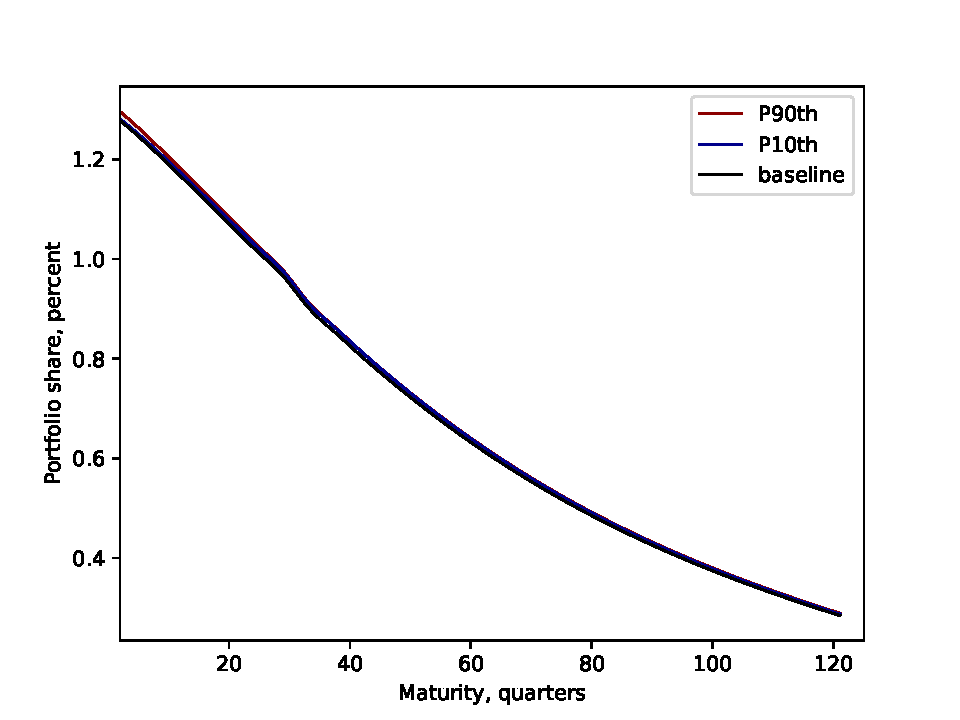
\includegraphics[scale=0.5]{figdata/fig_het}

\caption{\label{fig:90-10 het} 90-10 interval of portfolio shares (maturities
from 2 quarters to 120 quarters) with heteroskedastic shocks.}
\end{figure}


\paragraph*{Alternative, time aggregation, calculation of returns}

We also experimented with alternative ways to calculate returns with
different time frequencies. In the baseline, we used quarterly measures
of returns, surpluses and taxes to ensure the largest sample such
that we could measure asset prices and macro data in a consistent
way. To verify if our results are driven by our choice of the frequency,
we use returns and other macro variables at biannual frequencies.
The shortest maturity available is now of 6 months, which we take
as our measure of the one-period government bond $R_{t}^{rf}$. As
before, we construct the biannual holding period return by summing
monthly returns for each portfolio which are separated by 6 month
intervals. For other macro variables, we aggregate two consecutive
quarters to obtain the biannual series. Using this data, we apply
the same procedure as the baseline (extracting the factor, estimating
the factor model, constructing the conditional covariances) and obtain
the optimal portfolio. We show the implied unrestricted target portfolios
in Figure \ref{fig:Annual}. In order to compare it to our baseline
results which have portfolios by quarterly bins, we aggregate the
baseline portfolio weights to biannual weights using $\omega_{biannual}\left[i\right]\equiv\omega\left[2i-1\right]+\omega\left[2i\right]$,where
$i$ indexes the 6 month intervals and the right hand size is the
baseline target portfolio. We find that that the two biannual portfolios
are similar.

\begin{figure}
\centering{}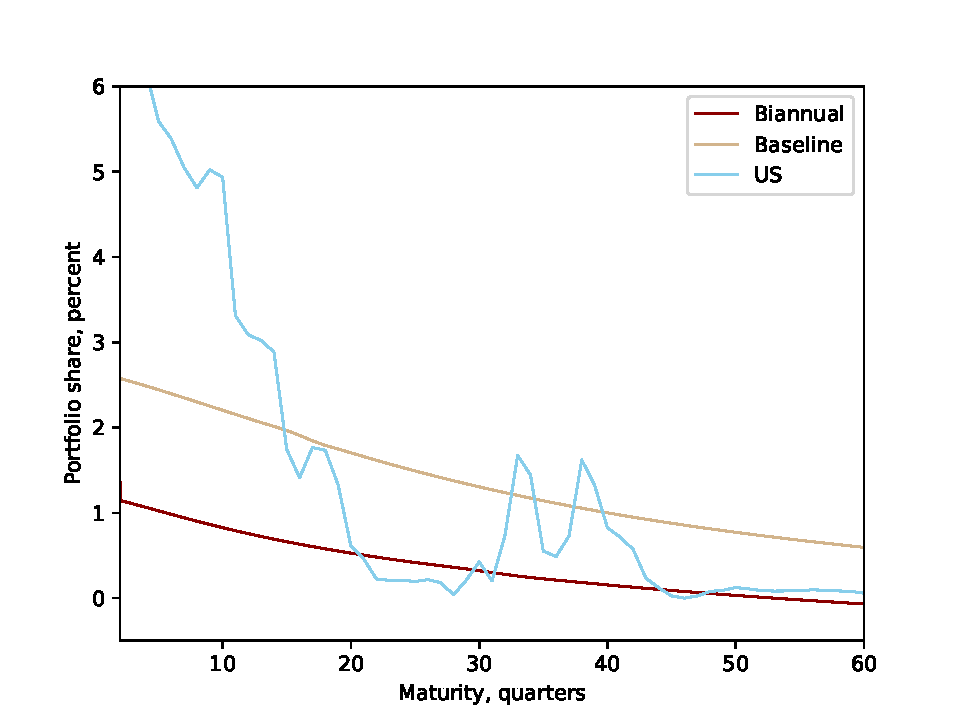
\includegraphics[width=0.5\paperwidth]{figdata/opt_biannual}\caption{Bi-annual frequency\label{fig:Annual}}
\end{figure}


\subsection{Additional details for Section \ref{subsec:Price-Effects} \label{subsec: price effects appendix}}

In this appendix, we document how we estimate $\Lambda_{t}$ using
estimates from \citet{GreenwoodVayanosRFS2014}.

\citeauthor{GreenwoodVayanosRFS2014} report estimates of semi-elasticities
$\left\{ Y_{t}\frac{\partial\ln\text{yields}_{t}^{k}}{\partial\text{Bond Supply}_{t}}\right\} _{k}$
by bond maturity for a subset of maturities using maturity-weighted
debt $\sum k\tilde{B}_{t}^{k}$ as a measure of bond supply. We assume
that weights $\tilde{\omega}_{t}^{k}=\frac{\tilde{B}_{t}^{k}}{\sum_{k}\tilde{B}_{t}^{k}}$
remain constant when $\sum k\tilde{B}_{t}^{k}$ changes. Under this
assumption, a unit change in $\sum k\tilde{B}_{t}^{k}$ leads to a
$\frac{1}{\tilde{\omega}_{t}^{k}}$ variation in supply of bond of
maturity $k$. Using the definition of $\Lambda_{t}$ from the text,
and converting the estimate of yields to prices, we get

\begin{equation}
D_{t}\Lambda_{t}[j,k]=\iota_{\{k=j\}}\left(\text{\ensuremath{\frac{\sum_{k=1}^{\infty}Q_{t}^{k}}{\left(Q_{t}^{1}\right)^{2}}\frac{\xi^{2}\left(\tau_{t}\right)}{-\xi^{\prime}\left(\tau_{t}\right)}}}\frac{}{Q_{t}^{k}}\right)\left(\frac{k\times\left\{ Y_{t}\frac{\partial\ln\text{yields}_{t}^{k}}{\partial\text{Bond Supply}_{t}}\right\} _{k}}{\omega_{t}^{US,k}}\right)\left(\frac{\sum k\tilde{B}_{t}^{US,k}}{B_{t}}\right)\label{eq: GV}
\end{equation}
where all the terms on the right-hand side are measurable.\footnote{\citeauthor{GreenwoodVayanosRFS2014} report elasticities $\left\{ Y_{t}\frac{\partial\ln\text{yields}_{t}^{k}}{\partial\text{Bond Supply}_{t}}\right\} _{k}$
for a subset of maturities. For an arbitrary maturity $n$, we assume
that the elasticity satisfies $a_{0}-a_{0}\exp\left\{ -a_{1}n^{2}\right\} $
where parameters $a_{0}$ capture the long run level and parameter
$a_{1}$ captures the speed of convergence. We fit $\left(a_{0},a_{1}\right)$to
match the long maturity elasticity of $0.003$ and the short maturity
(1 years) elasticity of $0.001$ from Table 3 in \citet{GreenwoodVayanosRFS2014}.
Since the \citeauthor{GreenwoodVayanosRFS2014} estimates are relatively
flat over the maturities, the exact interpolation scheme is not critical
of the results. We set $\left(\frac{\sum k\tilde{B}_{t}^{k}}{B_{t}}\right)$
to $7.3$ using the values reported in Panel A of Table 1 in \citet{GreenwoodVayanosRFS2014}.}

The first term in (\ref{eq: GV}) is obtained directly from estimates
of the price curve $\left\{ Q_{t}^{k}\right\} $and the tax rate $\tau_{t}$
and we set them to the same values we use in Section \ref{sec: target portfolio}.
To get the second term in (\ref{eq: GV}), we bin maturities in 5
year bins with the last bin for maturities greater than $15$ years.
The red dots in Figure \ref{fig: GV fit} are the implied values of
$\left\{ \left(\frac{k\times\left\{ Y_{t}\frac{\partial\ln\text{yields}_{t}^{k}}{\partial\text{Bond Supply}_{t}}\right\} _{k}}{\omega_{t}^{US,k}}\right)\left(\frac{\sum k\tilde{B}_{t}^{US,k}}{B_{t}}\right)\right\} _{k}$.
For intermediate maturities, we interpolate using the nearest value.
The bold line in Figure \ref{fig: GV fit} is the interpolated curve
that we use in our implementation. 
\begin{figure}
\centering{}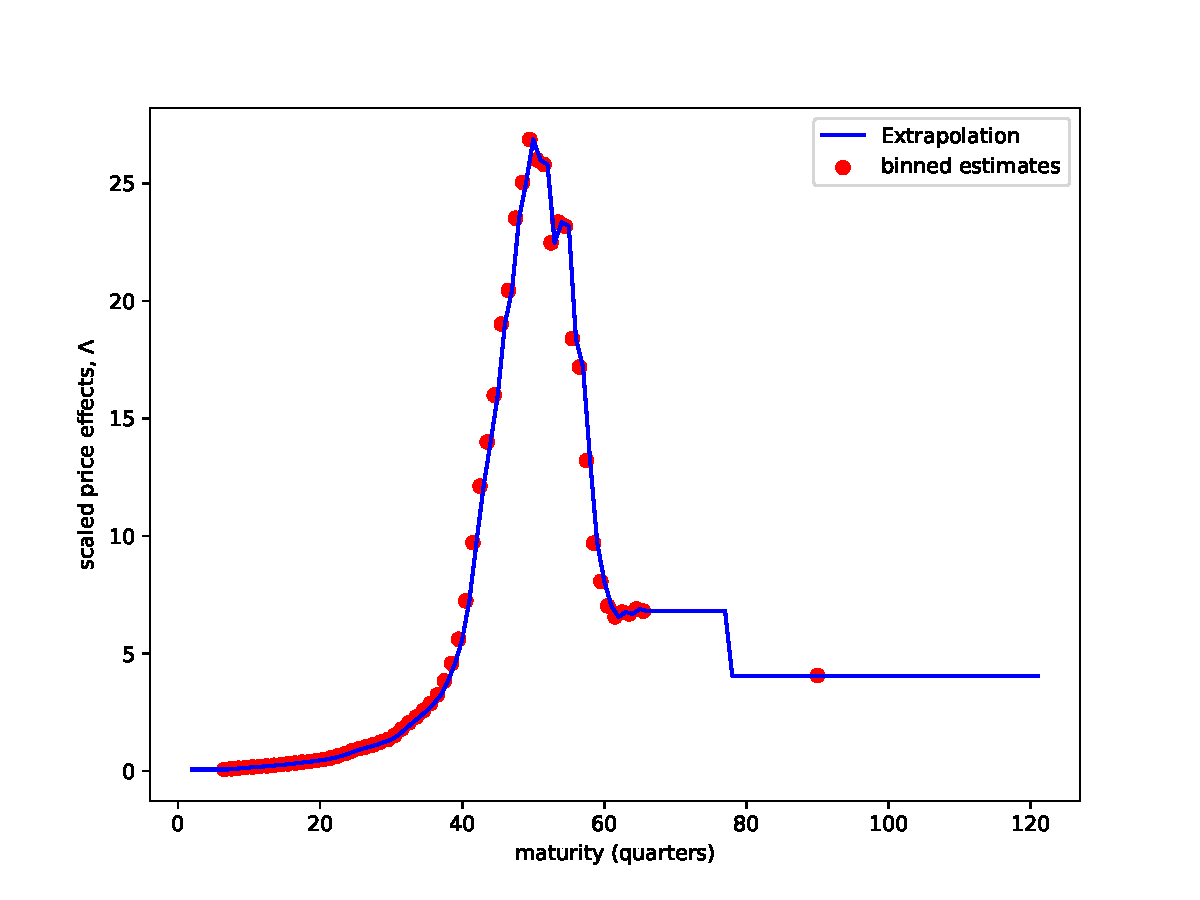
\includegraphics[width=0.5\paperwidth]{figdata/gv_fit}\caption{\label{fig: GV fit} Fit for price effect semi-elaticities. We use
5 year bins with the last bin $15+$ years to measure $\Lambda$.
The red dots indicated estimates of the right hand side of equation
\ref{eq: GV} for the bins. The blue solid line is interpolated values
that we use to measure all elements of $\Lambda_{t}$.}
\end{figure}

We then set $\Lambda_{t}$ constant across dates at the estimated
values and use equation (\ref{eq: price effects with costly bond without h})
to compute the steady state portfolio.

\subsection{Additional details for Section \ref{subsec:Imperfect-substitutes-empirical}
\label{subsec:Additional-details-for-imperfect substitutes and heterogenity}}

\paragraph{\protect 
%
}We can get a feel for how trading frictions affect the optimal portfolio
by studying a special case. We assume stationarity and set $Q_{t}^{k}=\beta^{k}$,
and further specialize to a simpler market structure in which the
government trades only a risk-free security and a growth-adjusted
consol. Let $\overrightarrow{\beta}$ be a geometrically declining
series $\beta^{k},\beta^{k-1},\ldots$ and excess return on the consol
be denoted by $r_{t}^{\infty}$. Finally, we impose that the stochastic
discount factor of the non-traders is scaled version of the stochastic
discount factor of the traders: $\ln\left(M_{\mathbb{N},t+k}\right)=(1+\psi)\ln\left(M_{\mathcal{\mathcal{\mathbb{T}}},t+k}\right).$
This introduces a new parameter, $\psi$, that captures the severity
of trading frictions as $\psi>0$ implies that the SDF of the non-traders
is more volatile of those of the traders.

Under this last assumption the covariance of the relative stochastic
discount factors simplifies to 
\[
\text{cov}_{t}\left(\ln\left(M_{\mathcal{\mathbb{T}},t+k}\right)-\ln\left(M_{\mathbb{N},t+k}\right),r_{t+1}^{j}\right)=-\psi\text{cov}_{t}\left(\ln\left(M_{\mathcal{\mathbb{T}},t+k}\right),r_{t+1}^{j}\right).
\]
As the traders trade the consol, we can use the traders' Euler equation,
equation \eqref{eq:EE_avgtrader}, to substitute out for this covariance
and obtain 
\[
-\text{cov}_{t}\left(\ln\left(M_{\mathcal{\mathcal{\mathbb{T}}},t+k}\right),r_{t+1}^{j}\right)\simeq\mathbb{E}_{t}r_{t+1}^{j}-\text{cov}_{t}\left(\ln Q_{t+1,t-1},r_{t+1}^{j}\right).
\]
 Under our stationarity assumptions we have $\mu_{\mathcal{N},t+k}=\mu_{\mathcal{N},t}$
and can therefore express $\Sigma_{t}^{M}$ as the sum of three terms
\[
\Sigma_{t}^{M}=\mu_{\mathbb{N},t}\psi\left(\mathcal{R}_{t}-\overline{Q}_{t}^{1}\Sigma_{t}^{Q}\right)
\]
 where $\mathcal{R}_{t}[j,k]=Q_{t}^{1}\mathbb{E}_{t}r_{k+1}^{j}.$

The effect of non-traders on the optimal portfolio is given by $\Sigma_{t}^{-1}\Sigma_{t}^{M}s_{t}^{ineq}.$
This simplifies under this market structure of a growth adjusted consol
and a risk free bond as $\Sigma_{t}$ is now a single number representing
the conditional covariance of the growth adjusted consol. We can also
make progress on the components of $\Sigma_{t}^{M}\overrightarrow{\beta},$
starting with $\mathcal{R}_{t}\overrightarrow{\beta}=\frac{\mathbb{E}_{t}r_{t+1}^{j}}{1-\beta}$
. Next we note that 
\begin{align*}
\Sigma_{t}^{Q}\overrightarrow{\beta}=\sum_{k=1}^{\infty}\beta^{t}\text{cov}_{t}\left(\frac{1}{Q_{t}^{1}}\ln Q_{t+1,k},r_{t+1}^{\infty}\right) & \simeq\frac{\Gamma}{\beta}\sum_{k=1}^{\infty}\beta^{t}\mathbb{E}_{t}\partial_{\sigma}\ln Q_{t+1,k}\partial_{\sigma}r_{t+1}^{\infty}\\
 & \simeq\frac{\Gamma}{\beta}\mathbb{E}_{t}\sum_{k=1}^{\infty}\Gamma^{t}\partial_{\sigma}Q_{t+1,k}\partial_{\sigma}r_{t+1}^{\infty}\\
 & \simeq\frac{\Gamma}{\beta}\mathbb{E}_{t}\partial_{\sigma}Q_{t+1}^{\infty}\partial_{\sigma}r_{t+1}^{\infty}\\
 & \simeq\frac{\Gamma}{1-\beta}\text{cov}_{t}(r_{t+1}^{\infty},r_{t+1}^{\infty})=\frac{\Gamma}{1-\beta}\Sigma_{t}.
\end{align*}
 All put together we have that 
\[
\Sigma_{t}^{-1}\Sigma_{t}^{M}\overrightarrow{\beta}\approx\frac{\mu_{\mathbb{N},t}\psi}{1-\beta}\left(\frac{\mathbb{E}_{t}r_{t+1}^{\infty}}{\text{var}_{t}(r_{t+1}^{\infty})}-\beta\right).
\]
 So the presence of non-traders will lengthen the maturity as long
as $\frac{\mathbb{E}_{t}r_{t+1}^{\infty}}{\text{var}_{t}(r_{t+1}^{\infty})}>\beta.$
We can construct estimates for both $\mathbb{E}_{t}r_{t+1}^{\infty}$
and $\text{var}_{t}(r_{t+1}^{\infty})$ using the fact that the growth
adjusted consol is the infinite sum of zero coupon bonds of all maturities
weighted by $\beta^{j}.$ To check the inequality, we use the estimates
of the factor model and find that the $\frac{\mathbb{E}_{t}r_{t+1}^{\infty}}{\text{var}_{t}(r_{t+1}^{\infty})}$
is indeed significantly larger that one and hence any reasonable estimate
of $\beta.$

\section{Additional details for Section \ref{sec: Comparing to neoclassical}\label{sec:appendix neoclassical portfolios }}

To simulate the neoclassical model, we solve a complete markets Ramsey
allocation as in \citet{LucasStokeyJME1983} by posing the following
maximization problem. Given some $t=0$ state $s_{0}\in\mathcal{S}$
and household savings $b_{0}\left(s^{0}\right),$ the Ramsey problem
can be expressed as 
\begin{equation}
\max_{c_{t}\left(s^{t}\right),y_{t}\left(s^{t}\right)}\mathbb{E}_{0}\sum_{t=0}^{\infty}u\left(C_{t},\frac{Y_{t}}{\theta_{t}}\right)\label{eq:abn objective}
\end{equation}
subject to 
\begin{equation}
Y_{t}\left(s^{t}\right)=C_{t}\left(s^{t}\right)+G\left(s_{t}\right),\label{eq:resource constraint}
\end{equation}

\begin{equation}
b_{0}\left(s^{0}\right)u_{c}\left(s^{0}\right)=\sum_{t=0}^{\infty}\sum_{s^{t}}\beta^{t}\pi_{t}\left(s^{t}\right)\left[u_{c}\left(s^{t}\right)C_{t}\left(s^{t}\right)+u_{y}\left(s^{t}\right)Y_{t}\left(s^{t}\right)\right],\label{implementability}
\end{equation}
where the \emph{implementability constraints,} equation (\ref{implementability})
is derived by taking the time-0 budget constraint and replacing after-tax
wages as well as bond prices.

We assume that the state space $\mathcal{S}$ is discrete (described
below) and non-linearly solve the optimal allocation using the first-order
conditions of the Ramsey planning problem. The resulting optimal allocation
is represented using two sets of vectors of dimension $2|\mathcal{S}|$,
one set for consumption and labor choices at $t=0$ and another set
for all $s_{t}\in\mathcal{S}$ for $t\ge1$. Using the Ramsey allocation
$\left\{ c_{t},y_{t}\right\} $, we can back out other related objects
such tax rates $\tau_{t}=1-\frac{\left(\frac{Y_{t}}{\theta_{t}}\right)^{\gamma}}{c_{t}^{-\sigma}}$
; primary surplus $X_{t}=\tau_{t}Y_{t}-G_{t}$; and zero-coupon bond
prices $Q_{t}^{n}=\mathbb{E}_{t}\frac{C_{t+n}^{-\sigma}}{C_{t}^{-\sigma}}.$

We follow \citet{BueraNicolini_etalJME2004} and assume that the preferences
of households are isoelastic $U\left(C_{t},\frac{Y_{t}}{\theta_{t}}\right)=\frac{C_{t}^{1-\sigma}}{1-\sigma}-\frac{\left(\frac{Y_{t}}{\theta_{t}}\right)^{1+\gamma}}{1+\gamma}$
with parameters $\sigma=2$ and $\gamma=1$. The economy is closed,
so the demand of assets from foreign investors is zero and there are
liquidity services provided by government bonds. The only source of
uncertainty comes from the exogenous stochastic process of government
expenditures $G_{t}$, which follows an AR(1) process 
\[
\ln G_{t}=\alpha_{G}+\rho_{G}\ln G_{t-1}+\sigma_{G}\epsilon_{t}
\]
 We set $\left(\alpha_{G},\rho_{G},\sigma_{G}\right)$ to obtain a
mean $G/Y$ of $15\%$, auto correlation of $0.95$ and a standard
deviation $\frac{1.2}{15}$ which are in line with the U.S. data that
we use in Section \ref{sec: Data Description}. We discretize the
$\ln G_{t}$ process with $|\mathcal{S}|=20$ grid points. For our
calculations, we set the level of initial debt $B_{0}$ so that the
annualized initial level of government liabilities to GDP is 100\%.

We use this parameterization to construct several versions of the
optimal portfolio. First, for a given $s\in\mathcal{S},$ we apply
Corollary to Theorem 1 in \citet{AngeletosQJE2002} and obtain the
optimal portfolio $\omega_{T}^{CM,n}\left(s^{T}\right)=\omega^{CM,n}\left(s_{T}=s\right)$
for $n=1,\ldots20$ maturities that implements the complete markets
allocation. We use the bond prices and present value of primary surpluses
all of which can be backed out given the objects from the Ramsey allocation.
In Figure \ref{fig: Government-portfolio-shares_Angeletos_and_us},
red color line, we plot $\left\{ \omega^{CM,n}\right\} _{n=1}^{20}$
for $s_{T}=s_{10}$ which is the modal state.

\paragraph{Details for Figure \ref{fig: Government-portfolio-shares_Angeletos_and_us}}

To obtain the target portfolio $\omega_{t}$ given some history $s^{t},$
we need to solve for a vector of portfolio shares that satisfies 
\[
\Sigma_{t}\mathbf{\omega}_{t}=\left[\Sigma_{t}^{Q}s_{t}^{Q}+\Sigma_{t}^{G}s_{t}^{G}\right].
\]
Before explaining how we get $\omega_{t}$, we make two observations.
First, given the properties of the Ramsey allocations, $\Sigma_{t},\Sigma_{t}^{Q}s_{t}^{Q},s_{t}^{G},\Sigma_{t}^{G}$
only depend on state $s_{t}$, which we set to $s_{10}$ and as before
can be computed in closed form using the complete market allocation
that we have already solved. Second, as mentioned in the main text
the returns of different bonds are highly correlated in the neoclassical
economy, which makes the matrix of returns $\Sigma_{t}$ to be effectively
non-invertible and there are a range of portfolios that satisfy inequality
(\ref{eq: tolerance}) for a given $\epsilon$. To obtain the target
portfolio that is plotted in Figure \ref{fig: Government-portfolio-shares_Angeletos_and_us}
blue color, we set $\epsilon=1e-8$ and pose the following minimization
problem 
\[
\min_{\tilde{\mathbf{\omega}}}\left\Vert \mathbf{\tilde{\omega}}-\omega_{t}^{ABN}\right\Vert 
\]
such that
\[
\left\Vert \Sigma_{t}\tilde{\omega}^{n}-\left[\Sigma_{t}^{Q}s_{t}^{Q}+\Sigma_{t}^{G}s_{t}^{G}\right]\right\Vert \leq\boldsymbol{1}^{\intercal}\epsilon.
\]
where $||\cdot\|$ we mean the sup norm . This formulation conveniently
delivers an objective that is quadratic while the constraint set is
linear and convex; and we use a standard methods (OSQP library) to
solve the minimization problem.

\section{Closed Economy\label{sec:Closed-Economy}}

In this appendix, we study a closed neoclassical version of our \textit{benchmark
economy}. Unlike the benchmark open economy specification in Section
\ref{sec: environment}, a change in the governments portfolio will
necessarily change the price of assets in economy; and, compared to
the segmented markets version of the benchmark economy presented in
Section \ref{sec: price impact}, a change in the portfolio composition
at date $t$ will also affect the price of securities in all other
periods.

In what follows, we show how to to adjust our variational approach
to incorporate such effects on prices. Our main result is to characterize
the price effects and using that we show that the closed economy neoclassical
setting implies price responses that are counterfactual relative to
the evidence reviewed in Section \ref{sec: price impact}. Besides
the different structure on price effects, the rest of the analysis
of a closed economy including the steps to obtain the expression for
the optimal portfolio are similar to Section \ref{sec: characerization benchmark}.
In Section \ref{subsec:Analysis closed economy}, we formally describe
the neoclassical closed economy environment that we study, then introduce
the perturbation and analyze the welfare effects and optimality of
the government. The proofs of the main results are in Section \ref{proofs for appendix C}.

\subsection{Analysis \label{subsec:Analysis closed economy}}

In addition to the assumptions of the benchmark economy we assume
that:
\begin{enumerate}
\item Household preferences are time separable 
\[
V_{t}=u_{t}\left(C_{t}-\frac{\left(Y_{t}/\theta_{t}\right)^{1+1/\gamma}}{1+1/\gamma}\right)+\beta\mathbb{E}_{t}V_{t+1}.
\]
\item Government expenditures $\left\{ G_{t}\right\} $ are exogenous.
\item All assets are in zero net supply.\footnote{That all assets are in zero net supply is for notational simplicity.
Assuming positive net supply simply adds another term to the resource
constraint equivalent to changing exogenous government expenditures.}
\item The set of available securities can replicate a consol. We will let
$Q_{t}^{\infty}$ denote the price of the consol at date $t$.
\end{enumerate}
%
Under these assumptions asset market clearing implies that
\[
b_{t}^{i}=B_{t}^{i}
\]
and 
\[
c_{t}+G_{t}=Y_{t}.
\]
Absence of trading frictions and non-pecuniary benefits of government
securities the household optimality conditions imply 
\begin{equation}
\mathbb{E}_{t}M_{t+1}R_{t+1}^{i}=M_{t}\text{ or }M_{t}Q_{t}^{i}=\mathbb{E}_{t}\left[M_{t+1}\left(d_{t+1}^{i}+Q_{t+1}^{i}\right)\right]\label{hh euler}
\end{equation}


\paragraph*{Perturbation}

Following Section \ref{sec: characerization benchmark}, we use a
perturbational approach to isolate the optimal public portfolio. The
perturbations in this section are slightly different and adapted to
get tractability in the closed economy environment.

We consider any competitive equilibrium and introduce a perturbation
at a particular history $s^{t}$ by assuming that the government purchases
$\frac{\epsilon}{Q_{t}^{j}(s^{t})}$ units of security $j$ which
is funded by selling $\frac{\epsilon}{Q_{t}^{1}(s^{t})}$ of the risk
free bond. This asset swap produces an additional $r_{t+1}^{j}(s^{t+1})\epsilon$
of excess returns at all histories $s^{t+1}$ following $s^{t}.$
We assume that the government uses those resources to purchase an
additional $\frac{r_{t+1}^{j}(s^{t})\epsilon}{1+Q_{t+1}^{\infty}(s^{t+1})}$
of the consol while keeping its holdings of all other assets constant.
Due to its nature of swapping a longer security for a risk-free bond
we will refer to this as a Quantitative Easing (or QE) perturbation
and formally define it by
\[
\partial_{QE}B_{t}^{i}(\tilde{s}^{\ell})=\begin{cases}
\frac{\epsilon}{Q_{t}^{1}(s^{t})} & \text{if \ensuremath{i=rf} and \ensuremath{\tilde{s}^{\ell}=s^{t}}},\\
-\frac{\epsilon}{Q_{t}^{j}(s^{t})} & \text{if \ensuremath{i=j} and \ensuremath{\tilde{s}^{\ell}=s^{t},}}\\
-\frac{1}{1+Q_{t+1}^{\infty}\left(s^{t}\right)}\left(r_{t+1}^{j}\left(s^{t+1}\right)\right)\epsilon & \text{if \ensuremath{i=\infty} and \ensuremath{\tilde{s}^{\ell}\succ s^{t},}\ensuremath{\ell>t},}\\
0 & \text{otherwise.}
\end{cases}
\]
 The change in portfolio composition necessarily requires a change
in taxes to balance the governments budget constraint,
\[
G_{t}+\sum_{i}(Q_{t}^{i}+d_{t}^{i})B_{t-1}^{i}=\tau_{t}Y_{t}+\sum_{i}Q_{t}^{i}B_{t}^{i}.
\]
 Differentiating with respect to $\epsilon$ in the direction of the
QE perturbation yields the following response of tax revenues
\begin{equation}
-\partial_{QE}\left(\tau_{\ell}Y_{\ell}\right)=\frac{r_{t+1}^{j}\left(s^{t+1}\right)}{1+Q_{t+1}^{\infty}\left(s^{t+1}\right)}\left(I_{\{s^{\ell}\succ s^{t}\}}\right)+\sum\partial_{\epsilon}Q_{\ell}^{i}(s^{\ell})\left(B_{\ell}^{i}(s^{\ell-1})-B_{\ell-1}^{i}(s^{\ell})\right)\label{eq: revenue effects-2}
\end{equation}
where $I_{\{s^{\ell}\succ s^{t}\}}$ is an indicator returning $1$
if history $s^{\ell}$ follows from $s^{t}$ and zero otherwise. Intuitively
the effect of the perturbation on tax revenues is a combination of
two effects. The first, $\frac{r_{t+1}^{j}\left(s^{t+1}\right)}{1+Q_{t+1}^{\infty}\left(s^{t+1}\right)}\left(I_{\{s^{\ell}\succ s^{t}\}}\right)$,
are the direct effects that are a result of the excess returns generated
by the asset swap. The second,$\sum\partial_{QE}Q_{\ell}^{i}(s^{\ell})\left(B_{\ell}^{i}(s^{\ell-1})-B_{\ell-1}^{i}(s^{\ell})\right)$,
is the indirect effect that arises because the asset swap in period
$t$ changes prices not only in all future periods but also in all
past periods starting from the initial date 0.

Assuming that the equilibrium manifold is sufficiently smooth, we
can apply the envelope theorem to the household's maximization problem
to obtain the welfare impact of this perturbation as $\epsilon\rightarrow0.$
The welfare effect of this perturbation comes from its effect on both
tax rates and security prices and is given by
\begin{align}
\partial_{QE}V_{0} & =\mathbb{E}_{0}\sum_{\ell\geq0}M_{\ell}\left(-\frac{\partial_{QE}\left(\tau_{\ell}Y_{\ell}\right)}{\xi_{\ell}}+\sum_{i\geq0}\partial_{QE}Q_{\ell}^{i}\left(b_{\ell-1}^{i}-b_{\ell}^{i}\right)\right)\nonumber \\
 & =\mathbb{E}_{0}\sum_{\ell\geq0}M_{\ell}\left(-\frac{\partial_{QE}\left(\tau_{\ell}Y_{\ell}\right)}{\xi_{\ell}}+\sum_{i\geq0}\partial_{QE}Q_{\ell}^{i}\left(B_{\ell-1}^{i}-B_{\ell}^{i}\right)\right)\nonumber \\
 & =\mathbb{E}_{0}\left[\sum_{\ell\geq0}M_{\ell}\sum_{i\geq0}\partial_{QE}Q_{\ell}^{i}\left(\frac{\xi_{\ell}B_{\ell-1}^{i}-B_{\ell-1}^{i}}{\xi_{\ell}}-\frac{\xi_{\ell}B_{\ell}^{i}-B_{\ell}^{i}}{\xi_{\ell}}\right)+\sum_{\ell\geq T+1}\left(\frac{M_{\ell}}{\xi_{\ell}}\right)\left(I_{\{\tilde{s}^{\ell}\succ s^{T}\}}\right)\left(\frac{r_{T+1}^{j}}{1+Q_{T+1}^{\infty}}\right)\right]\nonumber \\
 & =\mathbb{E}_{0}\left[\sum_{\ell\geq0}M_{\ell}\left(\frac{\xi_{\ell}-1}{\xi_{\ell}}\right)\sum_{i\geq0}\partial_{QE}Q_{\ell}^{i}\left(B_{\ell-1}^{i}-B_{\ell}^{i}\right)+\sum_{\ell\geq t+1}\left(\frac{M_{\ell}}{\xi_{\ell}}\right)\left(I_{\{\tilde{s}^{\ell}\succ s^{t}\}}\right)\left(\frac{r_{t+1}^{j}}{1+Q_{t+1}^{\infty}}\right)\right]\nonumber \\
 & =\mathrm{Pr}_{0}\left(s^{t}\right)M_{t}\left(s^{t}\right)\left[PE+\mathbb{E}_{t}\sum_{k\geq1}\left(\frac{M_{t+k}}{M_{t}}\right)\left(\frac{r_{t+1}^{j}}{1+Q_{t+1}^{\infty}}\right)\frac{1}{\xi_{t+k}}\right]\label{welfare effects}
\end{align}
wi$\ell$h
\[
PE=\frac{1}{\mathrm{Pr}_{0}\left(s^{t}\right)M_{T}\left(s^{t}\right)}\mathbb{E}_{0}\left[\sum_{\ell\geq0}M_{\ell}\left(\frac{\xi_{\ell}-1}{\xi_{\ell}}\right)\sum_{i\geq0}\partial_{QE}Q_{\ell}^{i}\left(B_{\ell-1}^{i}-B_{\ell}^{i}\right)\right].
\]
The term $\mathbb{E}_{t}\sum_{k\geq1}\left(\frac{M_{t+k}}{M_{t}}\right)\left(\frac{r_{t+1}^{j}}{1+Q_{t+1}^{\infty}}\right)\frac{1}{\xi_{t+k}}$
parallels the effect of the same perturbation in the open economy
benchmark model, and can be analyzed in a similar manner. Now, in
addition to that term, we also have $PE$ that captures the effect
on asset prices for all histories starting from time 0 onward. In
the next section we will show how our second order expansions can
allow us express that term using covariances that can be measured
in the data.

\paragraph*{Characterizing the Price Effects}

The perturbation affects asset prices through its effect on the stochastic
discount factor of the household. This can be seen by differentiating
the household Euler equation \eqref{hh euler} with respect to $\epsilon$
in the direction of the perturbation to get 
\[
\left(\partial_{QE}M_{\ell}\right)Q_{\ell}^{i}+M_{\ell}\left(\partial_{QE}Q_{\ell}^{i}\right)=\mathbb{E}_{\ell}\left[\partial_{QE}M_{\ell+1}\left(d_{\ell+1}^{i}+Q_{\ell+1}^{i}\right)+M_{\ell+1}\left(\partial_{QE}Q_{\ell+1}^{i}\right)\right].
\]
As the perturbation affects the stochastic discount factor through
changes in tax rates we define $\xi_{M,\ell}\equiv\frac{\partial\log M_{\ell}}{\partial\left(\tau_{\ell}y_{\ell}\right)}$
as the semi-elasticity of $\log M_{t}$ with respect to the tax revenues
which implies $\partial_{QE}M_{\ell}=M_{\ell}\xi_{M,\ell}\partial_{QE}\left(\tau_{\ell}y_{\ell}\right).$
Under our assumptions, this semi-elasticity is given by 
\[
\xi_{M,\ell}=-\psi_{\ell}\times\frac{1}{Y_{\ell}-G_{\ell}-\theta_{\ell}v\left(Y_{\ell}\right)}\times\left(\frac{\xi_{\ell}-1}{\xi_{\ell}}\right)
\]
where $\psi_{\ell}\equiv\frac{-\left[c_{\ell}-v_{\ell}\left(Y_{\ell}\right)\right]U^{''}\left(c_{\ell}-v_{\ell}\left(Y_{\ell}\right)\right)}{U^{'}\left(c_{\ell}-v_{\ell}\left(Y_{\ell}\right)\right)}$
is the coefficient of relative risk aversion.

To get a better understanding of how these terms contribute the price
effects in the closed economy we'll focus on a stationary version
of the economy
\begin{defn}
An optimal competitive equilibrium is\textit{ stationary from time
$t$} if there exists a constant $R_{t}$ such that for all $\ell>t$
(i) $\mathbb{E}_{t}G_{\ell}\approx G_{t}$ (iii) $\mathbb{E}_{t}R_{\ell}^{i}\approx R_{t}$
for all $i$ and (iv) $\mathbb{E}_{t}c_{\ell}\approx c_{t}.$

This definition of stationary differs from the stationarity of the
main text in that we assume a growth rate of $\Gamma=1.$ All of our
results extend to a positive growth rate assuming that the utility
function is CRRA.\footnote{The main difference is that we will require that the government smooth
excess returns using a growth-adjusted consol rather than a pure consol.} Our first set of results concern the asset pricing implications of
the QE perturbation. We will leave the proof of both propositions
to the end of the section.
\end{defn}
\begin{prop}
\label{price effects CRRA} For a neoclassical model which is stationary
from time $t$
\end{prop}
\begin{enumerate}
\item The QE perturbation keeps asset prices zero to the first-order
\[
\partial_{\sigma}\partial_{QE}Q_{\ell}^{i}=0\quad\forall\quad i,\ell\geq0
\]
\item The QE perturbation only affects risk-premia at $t$
\[
\mathbb{E}_{\ell}\partial_{\sigma\sigma}\partial_{QE}r_{\ell+1}^{i}=0\quad\forall\quad\ell\neq t
\]
and at date $\ell$ 
\[
\mathbb{E}_{\ell}\partial_{\sigma\sigma}\partial_{QE}r_{\ell+1}^{i}=\frac{2\psi_{t}}{Y_{t}-G_{t}-\theta_{t}v\left(Y_{t}\right)}\times\left(\frac{1-\xi_{t}}{\xi_{t}}\right)\left(\frac{1}{1+\overline{Q}_{t+1}^{\infty}}\right)\mathbb{E}_{\ell}\partial_{\sigma}r_{\ell+1}^{j}\partial_{\sigma}r_{\ell+1}^{i}>0,
\]
where $\psi_{t}$ is coefficient of relative risk aversion.
\end{enumerate}
%
This proposition states that the QE perturbation does not effect prices
to zeroth or first order. This is inline with our modeling of price
effects in Section \ref{sec: price impact} where we assume that the
effect prices is at second order. Intuitively, to zeroth and first-order
all assets have the same expected return so the QE perturbation only
changes the risk profile of the household's stochastic discount factor
which, in turn, will only effect prices to second order. Moreover,
the proposition states that the effect on asset prices in the closed
economy are counterfactual to what has been documented in the data.
Estimates by \citet{GreenwoodVayanosRFS2014} and others find that
find that $\Lambda^{QE}[rf,j]\approx0$ and $\Lambda^{QE}[i,j]>0$
for $i>rf$ which implies that expected excess returns should decrease
with the QE perturbation rather than increase: 
\[
\mathbb{E}_{t}\partial_{\sigma\sigma}\partial_{QE}r_{t+1}^{i}=-\frac{\overline{Q}_{t+1}^{i}}{\overline{Q}_{t}^{i}}\frac{\partial_{\sigma\sigma}\partial_{QE}Q_{t}^{i}}{\overline{Q}_{t}^{i}}<0.
\]
When governments buy back long term debt by issuing short term debt,
short term rates appear to be unchanged so expected excess returns
are driven by the fall in the term premia as the increased demand
drives up prices. In contrast, in the closed economy, the government
returns the excess returns from the QE swap via taxes which results
in making states of the world where excess returns are high (low)
better (worse) for the household by lowering (raising) tax rates in
those states. As a result, the value of the asset decreases which
raises the risk-premia. As noted, this is in inconsistent with the
segmented market literature which finds that the excess returns on
long maturity debt are lower after QE. Finally, we are able to use
our expansions to characterize the price effects
\begin{prop}
\label{prop:price_effects_closed}For a neoclassical economy which
is stationary from time 0, if all initial debt $\left\{ B_{-1}^{i}\right\} _{i}$
was risk-free then $PE\simeq\left(\frac{\overline{\xi}}{\overline{\xi}-1}\right)^{-1}\varPsi_{t}\left(s^{t}\right)$
where
\begin{align*}
\varPsi_{t}\left(s^{t}\right)= & \frac{-2\overline{B}\overline{\xi}_{M}(\overline{Q}^{1}-1)}{\left(1-\overline{B}(\overline{Q}^{1}-1)\overline{\xi}_{M}\right)}\sum_{\ell=t+1}^{\infty}\left(\frac{\left(\overline{Q}_{t}^{1}\right)^{\ell-t}}{1+\overline{Q}_{t+1}^{\infty}}\right)cov_{t}\left(\partial_{\sigma}\ln M_{\ell},\partial_{\sigma}r_{t+1}^{j}\right)\\
 & -\frac{2\overline{\xi}_{M}\overline{B}}{\left(1-\overline{B}(\overline{Q}^{1}-1)\overline{\xi}_{M}\right)}\sum_{\ell=t+1}\left(\frac{\left(\overline{Q}_{t}^{1}\right){}^{-t}}{1+\overline{Q}_{t+1}^{\infty}}\right)cov_{t}\left(\partial_{\sigma}r_{t+1}^{j},\partial_{\sigma}\ln Q_{\ell}^{1}\right)\\
 & -\frac{2\overline{\xi}_{M}}{\left(1-\overline{B}(\overline{Q}^{1}-1)\overline{\xi}_{M}\right)}\sum_{j\geq1}\text{\ensuremath{\frac{\overline{Q}_{t}^{1}}{1+\overline{Q}_{t+1}^{\infty}\left(\ell^{t+1}\right)}}}cov_{t}\left(\partial_{\sigma}r_{t+1}^{j},\partial_{\sigma}r_{t+1}^{j}\right)\\
 & -\frac{2\overline{B}}{\left(1-\overline{B}(\overline{Q}^{1}-1)\overline{\xi}_{M}\right)}\sum_{\ell=t}^{\infty}\left(\frac{\left(\overline{Q}_{\ell}^{1}\right)^{\ell-t}}{1+\overline{Q}_{t+1}^{\infty}}cov_{t}\left(\partial_{\sigma}\xi_{M,\ell}-\partial_{\sigma}\xi_{M,\ell+1},\partial_{\sigma}r_{t+1}^{j}\right)\right)
\end{align*}
\end{prop}
As we have noted without any assumptions price effects are given by
\[
PE=\frac{1}{\mathrm{Pr}_{0}\left(s^{t}\right)M_{T}\left(s^{t}\right)}\mathbb{E}_{0}\left[\sum_{\ell\geq0}M_{\ell}\left(\frac{\xi_{\ell}-1}{\xi_{\ell}}\right)\sum_{i\geq0}\partial_{QE}Q_{\ell}^{i}\left(B_{\ell-1}^{i}-B_{\ell}^{i}\right)\right]
\]
where a swap of securities at a particular history can affect asset
prices at all other histories---past and future---due to general
equilibrium effects on the stochastic discount factor that now directly
depends on the tax rates. Proposition \ref{prop:price_effects_closed}
allows us to characterize these price effects with a closed form expression
using entirely time $t$ covariances that are measurable in the data.

\subsection{Proofs for Propositions \ref{price effects CRRA} and \ref{prop:price_effects_closed}
\label{proofs for appendix C}}

\subsubsection{Proof of Proposition \ref{price effects CRRA}}

We begin by noting that at the zeroth order, we get $\overline{\xi}_{M,\ell}^{j}=-\frac{\overline{\psi_{\ell}}}{\overline{Y}_{\ell}-\overline{G}_{\ell}-\overline{\theta}_{\ell}v\left(\overline{Y}_{\ell}\right)}\times\left(\frac{\overline{\xi}_{\ell}-1}{\overline{\xi}_{\ell}}\right)=\overline{\xi}_{M,t},$
is independent of time and the details of the perturbation. We proceed
by proving a series of lemmas documenting the results of Proposition
\ref{price effects CRRA}

\begin{lem}
\label{lem:zero expected returns}Expected excess returns are zero
to the zeroth and the first order
\end{lem}
\begin{proof}
The zeroth of (\ref{hh euler}) gives us 
\[
\overline{r}_{\ell+1}^{i}=0
\]
 Take first order expansion to get 
\[
\mathbb{E}_{\ell}\partial_{\sigma}r_{\ell+1}^{i}\overline{M_{\ell+1}}+\mathbb{E}_{\ell}\overline{r_{\ell+1}^{i}}\partial_{\sigma}M_{\ell+1}=0
\]
and thus
\[
\mathbb{E}_{\ell}\partial_{\sigma}r_{\ell+1}^{i}=0.
\]
\end{proof}
\begin{lem}
\label{price effects zero to first order} To the first order, price
effects are zero, that is, for all $i$, $\ell$: $\partial_{\sigma}\partial_{QE}Q_{\ell}^{i}=0$
\end{lem}
\begin{proof}
Start from the definition of $Q_{\ell}^{i}$
\[
Q_{\ell}^{i}\left(s^{\ell}\right)=\mathbb{E}_{s^{\ell}}\sum_{k\geq1}\frac{M_{\ell+k}}{M_{\ell}}D_{\ell+k}^{i}.
\]
\begin{comment}
\[
\partial_{\sigma}\partial_{QE}q_{t}=\mathbb{E}_{t}\sum_{k\geq1}\left(\frac{\partial_{\sigma}\partial_{QE}M_{T+k}}{\overline{M}_{t}}-\frac{\partial_{\sigma}M_{T+k}\overline{\partial_{QE}M_{t}}}{M_{t}^{2}}-\frac{\overline{M_{T+k}}\partial_{\sigma}\partial_{QE}M_{t}}{M_{t}^{2}}+\frac{\overline{M_{T+k}\partial_{QE}M_{t}}}{M_{t}^{4}}\partial_{\sigma}M_{t}^{2}\right)d_{T+k}.
\]
\[
\partial_{\sigma}\partial_{QE}q_{t}=\mathbb{E}_{t}\sum_{k\geq1}\left(\frac{\partial_{\sigma}\partial_{QE}M_{T+k}}{\overline{M}_{t}}-\frac{\overline{M_{T+k}}\partial_{\sigma}\partial_{QE}M_{t}}{\overline{M}_{t}^{2}}\right)d_{T+k}.
\]
\[
\partial_{\sigma}\partial_{QE}q_{t}=\mathbb{E}_{t}\sum_{k\geq1}\left(\frac{\partial_{\sigma}\partial_{QE}M_{T+k}}{\overline{M_{T+k}}}-\frac{\partial_{\sigma}\partial_{QE}M_{t}}{\overline{M}_{t}}\right)\left(\frac{\overline{M_{T+k}}}{\overline{M}_{t}}\right)d_{T+k}.
\]
Can we write $\frac{\partial_{\sigma}\partial_{QE}M_{T+k}}{\overline{M_{T+k}}}$
in logs?
\[
\frac{\partial_{\sigma}\partial_{QE}M_{T+k}}{\overline{M_{T+k}}}=\partial_{QE}\left(\frac{\partial_{\sigma}M_{T+k}}{\overline{M_{T+k}}}\right)=\partial_{QE}\partial_{\sigma}\log M_{T+k}
\]
\end{comment}
\[
\partial_{\sigma}\partial_{QE}Q_{\ell}^{i}=\mathbb{E}_{\ell}\sum_{k\geq1}\left(\partial_{QE}\partial_{\sigma}\log M_{\ell+k}-\partial_{QE}\partial_{\sigma}\log M_{\ell}\right)\left(\frac{\overline{M_{\ell+k}}}{\overline{M}_{t}`}\right)D_{\ell+k}^{i}.
\]
A necessary and sufficient condition for price effects to be zero
at the first order is that $k\geq1$
\begin{equation}
\mathbb{E}_{\ell}\left(\partial_{QE}\partial_{\sigma}\log M_{\ell+k}-\partial_{QE}\partial_{\sigma}\log M_{\ell}\right)=0\label{eq: change in log sdf first-order-1}
\end{equation}
Use the definition of $\xi_{M}\left(s^{\ell}\right)$ to get $\partial_{QE}\log M_{\ell}\left(s^{\ell}\right)=\partial_{QE}\left(\tau_{\ell}\left(s^{\ell}\right)Y_{\ell}\left(s^{\ell}\right)\right)\times\xi_{M}\left(s^{\ell}\right)$.
To first order 
\[
\partial_{\sigma}\partial_{QE}\log M_{\ell}=\partial_{\sigma}\partial_{QE}\left(\tau_{\ell}Y_{\ell}\right)\times\overline{\xi}_{M,\ell}
\]
Then (\ref{eq: change in log sdf first-order-1}) is equivalently
expressed as 
\begin{align*}
\mathbb{E}_{\ell}\left(\partial_{\sigma}\partial_{QE}\log M_{\ell+k}-\partial_{\sigma}\partial_{QE}\log M_{\ell}\right) & =\overline{\xi}_{M,\ell}\left(\mathbb{E}_{\ell}\partial_{\sigma}\partial_{QE}\left(\tau_{\ell+k}Y_{\ell+k}\right)-\partial_{\sigma}\partial_{QE}\left(\tau_{\ell}Y_{\ell}\right)\right)
\end{align*}
We check condition (\ref{eq: change in log sdf first-order-1}) by
guess and verify.

Suppose $\partial_{\sigma}\partial_{QE}Q_{\ell}^{i}=0$ for $\ell\geq0$,
then for all $\ell\geq0$ and from equations (\ref{eq: revenue effects-2})
\[
-\partial_{\sigma}\partial_{QE}\left(\tau_{\ell}Y_{\ell}\right)=\partial_{\sigma}\left(\frac{r_{t+1}^{j}\left(s^{t+1}\right)}{1+Q_{t+1}^{\infty}\left(s^{t+1}\right)}\right)I_{\{s^{\ell}\succ s^{t+1}\}}=\frac{\partial_{\sigma}r_{t+1}^{j}\left(s^{t+1}\right)}{1+\overline{Q}_{t+1}^{\infty}}I_{\{s^{t}\succ s^{t+1}\}}
\]
When $\ell\geq t+1$
\[
\mathbb{E}_{\ell}\left(\partial_{\sigma}\partial_{QE}\log M_{t+1+k}-\partial_{\sigma}\partial_{QE}\log M_{t+1}\right)=\overline{\xi}_{M,t+1}\left(\frac{\partial_{\sigma}r_{t+1}^{j}\left(s^{t+1}\right)}{1+\overline{Q}_{t+1}^{\infty}}-\frac{\partial_{\sigma}r_{t+1}^{j}\left(s^{t+1}\right)}{1+\overline{Q}_{t+1}^{\infty}}\right)I_{\{s^{\ell}\succ s^{t+1}\}}=0
\]
When $\ell\leq t$, we can use the fact that to the first order, expected
excess returns are zero from Lemma \textbf{(}\ref{price effects zero to first order})
to establish that (\ref{eq: change in log sdf first-order-1}) holds.
\end{proof}
%
\begin{lem}
\label{lem:risk premia}In the closed economy the effect of the perturbation
on expected excess returns is
\[
\mathbb{E}_{\ell}\partial_{\sigma\sigma}\partial_{QE}r_{\ell+1}^{i}=0\quad\forall\quad\ell\neq t
\]
and at date $t$ 
\[
\mathbb{E}_{t}\partial_{\sigma\sigma}\partial_{QE}r_{t+1}^{i}=\frac{2\psi_{t}}{Y_{t}-G_{t}-\theta_{t}v\left(Y_{t}\right)}\times\left(\frac{1-\xi_{t}}{\xi_{t}}\right)\left(\frac{1}{1+\overline{Q}_{t+1}^{\infty}}\right)\mathbb{E}_{\ell}\partial_{\sigma}r_{\ell+1}^{j}\partial_{\sigma}r_{\ell+1}^{i}>0
\]
\end{lem}
\begin{proof}
The first order expansion $\partial_{QE}M_{\ell}$ after using Lemma
\ref{price effects zero to first order} gives us
\[
\partial_{\sigma}\partial_{QE}M_{\ell+1}=-\overline{\xi}_{M,\ell}\overline{M}_{\ell+1}\left\{ \partial_{\sigma}\left(\frac{r_{t+1}^{j}}{1+Q_{t+1}^{\infty}}\right)I_{\{\boldsymbol{s}{}^{\ell}\succ\boldsymbol{s}^ {}{}^{t+1}\}}\right\} 
\]
Use this along with the second order expansion of households optimality
condition (\ref{hh euler}) to obtain 
\[
0=\mathbb{E}_{\ell}\partial_{\sigma}r_{\ell+1}^{i}\left(-\overline{\xi}_{M,\ell}\overline{M}_{\ell+1}\left\{ \partial_{\sigma}\left(\frac{r_{t+1}^{j}}{1+q_{t+1}^{\infty}}\right)I_{\{\boldsymbol{s}{}^{\ell}\succ\boldsymbol{s}{}^{t+1}\}}\right\} \right)+\mathbb{E}_{\ell}\partial_{\sigma\sigma}\partial_{QE}r_{\ell+1}^{i}\overline{M}_{\ell+1}
\]
For $\ell<t$, $I_{\{\boldsymbol{s}{}^{\ell}\succ\boldsymbol{s}{}^{t+1}\}}=0$
and thus $\mathbb{E}_{\ell}\partial_{\sigma\sigma}\partial_{QE}r_{\ell+1}^{i}=0$.

For $\boldsymbol{s}{}^{\ell}\succ\boldsymbol{s}{}^{t+1}$, use Law
of iterated expectations to get
\[
0=\mathbb{E}_{t+1+k}\partial_{\sigma}r_{t+1+k}^{i}\left(-\overline{\xi}_{M,t+1+k}\overline{M}_{t+1+k}\underbrace{\mathbb{E}_{t+1}\left\{ \partial_{\sigma}\left(\frac{r_{t+1}^{j}}{1+Q_{t+1}^{\infty}}\right)\right\} }_{=0}\right)+\mathbb{E}_{t+1+k}\partial_{\sigma\sigma}\partial_{QE}r_{t+k+2}^{i}\overline{M}_{t+2+k}
\]
and use Lemma \textbf{(}\ref{price effects zero to first order})
to get $\mathbb{E}_{\ell}\partial_{\sigma\sigma}\partial_{QE}r_{\ell+1}^{i}=0$
for $\boldsymbol{s}{}^{\ell}\succ\boldsymbol{s}{}^{t+1}$.

Finally for $\ell=t$
\[
0=\mathbb{E}_{t}\partial_{\sigma}r_{t+1}^{i}\left(-\overline{\xi}_{M,t}\overline{M}_{t+1}\left\{ \partial_{\sigma}\left(\frac{r_{t+1}^{j}}{1+q_{t+1}^{\infty}}\right)\right\} \right)+\mathbb{E}_{\ell}\partial_{\sigma\sigma}\partial_{QE}r_{\ell+1}^{i}\overline{M}_{t+1}.
\]
Substitute for $\overline{\xi}_{M,t}$ and simplify to to get 
\[
\mathbb{E}_{t}\partial_{\sigma\sigma}\partial_{QE}r_{t+1}^{i}\simeq\frac{2\psi_{t}}{Y_{t}-G_{t}-\theta_{t}v\left(Y_{t}\right)}\times\left(\frac{1-\xi_{t}}{\xi_{t}}\right)\left(\frac{1}{1+\overline{Q}_{t+1}^{\infty}}\right)\mathbb{E}_{\ell}\partial_{\sigma}r_{t+1}^{j}\partial_{\sigma}r_{\ell+1}^{i}.
\]
Since $\xi_{t}=1-\gamma\frac{\tau_{t}}{1-\tau_{t}}<1$, $Y_{t}-G_{t}-\theta_{t}v\left(Y_{t}\right)>0$
from Inada conditions, and $\psi_{t}>0$, we get that $\mathbb{E}_{t}\partial_{\sigma\sigma}\partial_{QE}r_{t+1}^{j}>0$.
\end{proof}

\subsubsection{Proof of Proposition \ref{prop:price_effects_closed}}

The second order expansion of the price effects
\begin{equation}
\partial_{\sigma\sigma}\left(\mathrm{Pr}_{0}\left(s^{t}\right)M_{t}\left(s^{t}\right)PE_{j,t,\epsilon}\right)=\mathbb{E}_{0}\left[\sum_{\ell\geq0}\left(\frac{\overline{\xi}_{\ell}-1}{\overline{\xi}_{\ell}}\right)M_{\ell}\sum_{i\geq0}\partial_{\sigma\sigma}\partial_{QE}Q_{\ell}^{i}\left(\overline{B}_{\ell-1}^{i}-\overline{B}_{\ell}^{i}\right)\right]\label{eq:crazy_1}
\end{equation}
which equals %
\begin{comment}
\begin{align*}
\mathbb{E}_{0}\left[\sum_{\ell\geq0}\sum_{i\geq0}\overline{B}_{\ell}^{i}\left(\overline{M}_{\ell+1}\partial_{\sigma\sigma}\partial_{QE}Q_{\ell+1}^{i}-\overline{M}_{\ell}\partial_{\sigma\sigma}\partial_{QE}Q_{\ell}^{i}\right)\right]+\overline{M}_{0}\sum_{i\geq0}\partial_{\sigma\sigma}\partial_{QE}Q_{0}^{i}\overline{B}_{-1}^{i} & =\overline{M}_{0}\sum_{i\geq0}\partial_{\sigma\sigma}\partial_{QE}Q_{0}^{i}\overline{B}_{-1}^{i}+\mathbb{E}_{0}\left[\sum_{\ell\geq0}\sum_{i\geq0}\overline{B}_{\ell}^{i}\overline{M}_{\ell+1}\partial_{\sigma\sigma}\partial_{QE}Q_{\ell+1}^{i}-\sum_{\ell\geq0}\sum_{i\geq0}\overline{B}_{\ell+1}^{i}\overline{M}_{\ell+1}\partial_{\sigma\sigma}\partial_{QE}Q_{\ell+1}^{i}-\sum_{i\geq0}\overline{B}_{0}^{i}\overline{M}_{0}\partial_{\sigma\sigma}\partial_{QE}Q_{0}^{i}\right]\\
 & =\mathbb{E}_{0}\left[\sum_{\ell\geq0}\sum_{i\geq0}\left(\overline{B}_{\ell}^{i}-\overline{B}_{\ell+1}^{i}\right)\overline{M}_{\ell+1}\partial_{\sigma\sigma}\partial_{QE}Q_{\ell+1}^{i}+\overline{M}_{0}\sum_{i\geq0}\partial_{\sigma\sigma}\partial_{QE}Q_{0}^{i}\overline{B}_{-1}^{i}-\sum_{i\geq0}\overline{B}_{0}^{i}\overline{M}_{0}\partial_{\sigma\sigma}\partial_{QE}Q_{0}^{i}\right]\\
 & =\mathbb{E}_{0}\left[\sum_{\ell\geq0}\overline{M}_{\ell}\sum_{i\geq0}\partial_{\sigma\sigma}\partial_{QE}Q_{\ell}^{i}\left(\overline{B}_{\ell-1}^{i}-\overline{B}_{\ell}^{i}\right)\right]
\end{align*}
\end{comment}
\begin{equation}
\left(\frac{\overline{\xi}_{0}-1}{\overline{\xi}_{0}}\right)\overline{M}_{0}\sum_{i\geq0}\partial_{\sigma\sigma}\partial_{QE}Q_{0}^{i}\overline{B}_{-1}^{i}+\left(\frac{\overline{\xi}_{0}-1}{\overline{\xi}_{0}}\right)\mathbb{E}_{0}\left[\sum_{t\geq0}\sum_{i\geq0}\overline{B}_{t}^{i}\left(\overline{M}_{t+1}\partial_{\sigma\sigma}\partial_{QE}Q_{t+1}^{i}-\overline{M}_{t}\partial_{\sigma\sigma}\partial_{QE}Q_{t}^{i}\right)\right].\label{pe inn terms of prices}
\end{equation}
Its easy to see that $\left(\frac{\overline{\xi}_{0}-1}{\overline{\xi}_{0}}\right)\overline{M}_{0}\sum_{i\geq0}\partial_{\sigma\sigma}\partial_{QE}Q_{0}^{i}\overline{B}_{-1}^{i}=\left(\frac{\overline{\xi}_{0}-1}{\overline{\xi}_{0}}\right)\overline{M}_{0}\sum_{i\neq1}\partial_{\sigma\sigma}\partial_{QE}Q_{0}^{i}\overline{B}_{-1}^{i}=0$
under the assumption that initial debt was risk-free.

$t$he household pricing equation implies
\begin{equation}
M_{\ell}Q_{\ell}^{i}=\mathbb{E}_{\ell}\left[M_{\ell+1}\left(Q_{\ell+1}^{i}+D_{\ell+1}^{i}\right)\right]\label{eq: hh euler equation}
\end{equation}
Differentiating by $\partial_{QE}$ gives
\[
\left(\partial_{QE}M_{\ell}\right)Q_{\ell}^{i}+M_{\ell}\partial_{QE}Q_{\ell}^{i}=\mathbb{E}_{\ell}\left[\left(\partial_{QE}M_{\ell+1}\right)\left(Q_{\ell+1}^{i}+D_{\ell+1}^{i}\right)+M_{\ell+1}\partial_{QE}Q_{\ell+1}^{i}\right]
\]
 Let's start by looking at $\ell<t$ , We know that $\partial_{\sigma}\partial_{QE}M_{\ell+1}=0$
so taking the second derivative with respect to $\sigma$ yields%
\begin{comment}
\[
\left(\partial_{\sigma\sigma}\partial_{QE}M_{t}\right)\overline{Q}_{t}^{i}+\overline{M}_{t}\partial_{\sigma\sigma}\partial_{QE}Q_{t}^{i}=\mathbb{E}_{t}\left[\left(\partial_{\sigma\sigma}\partial_{QE}M_{t+1}\right)\left(\overline{Q}_{t+1}^{i}+D_{t+1}^{i}\right)+\overline{M}_{t+1}\partial_{\sigma\sigma}\partial_{QE}Q_{t+1}^{i}\right]
\]
or 
\[
\mathbb{E}_{t}\left[\overline{M}_{t+1}\partial_{\sigma\sigma}\partial_{QE}Q_{t+1}^{i}-\overline{M}_{t}\partial_{\sigma\sigma}\partial_{QE}Q_{t}^{i}\right]=\mathbb{E}_{t}\left[\left(\partial_{\sigma\sigma}\partial_{QE}M_{t}\right)\overline{Q}_{t}^{i}-\left(\partial_{\sigma\sigma}\partial_{QE}M_{t+1}\right)\left(\overline{Q}_{t+1}^{i}+D_{t+1}^{i}\right)\right]
\]
or
\end{comment}
\[
\mathbb{E}_{\ell}\left[\overline{M}_{\ell+1}\partial_{\sigma\sigma}\partial_{QE}Q_{\ell+1}^{i}-\overline{M}_{\ell}\partial_{\sigma\sigma}\partial_{QE}Q_{\ell}^{i}\right]=\overline{Q}_{\ell}^{i}\mathbb{E}_{\ell}\left[\left(\partial_{\sigma\sigma}\partial_{QE}M_{\ell}\right)-\left(\partial_{\sigma\sigma}\partial_{QE}M_{\ell+1}\right)\overline{R}_{\ell+1}^{rf}\right].
\]
For $\ell>t$ and $s^{\ell}\succ s^{t}$ we have $\frac{\partial_{QE}M_{\ell}}{M_{\ell}}=\xi_{M,\ell}^{j}\partial_{QE}\left(\tau_{\ell}Y_{\ell}\right)$
and hence $\partial_{\sigma}\partial_{QE}M_{\ell}=\overline{M}_{\ell}\overline{\xi}_{M,\ell}\frac{\partial_{\sigma}r_{t+1}^{j}}{1+\overline{Q}_{t+1}^{\infty}}.$
The second order expansion of equation (\ref{eq: hh euler equation})
is
\begin{align*}
2\partial_{\sigma}\partial_{QE}M_{\ell}\partial_{\sigma}Q_{\ell}^{i}+\left(\partial_{\sigma\sigma}\partial_{QE}M_{\ell}\right)\overline{Q}_{\ell}^{i}+\overline{M}_{\ell}\partial_{\sigma\sigma}\partial_{QE}Q_{\ell}^{i} & =\mathbb{E}_{\ell}\left[2\partial_{\sigma}\partial_{QE}M_{\ell+1}\partial_{\sigma}\left(Q_{\ell+1}^{i}+D_{\ell+1}^{i}\right)\right]\\
 & +\left(\partial_{\sigma\sigma}\partial_{QE}M_{\ell+1}\right)\left(\overline{Q}_{\ell+1}^{i}+D_{\ell+1}^{i}\right)+\overline{M}_{\ell+1}\partial_{\sigma\sigma}\partial_{QE}Q_{\ell+1}^{i}
\end{align*}
We know that$t$ 
\[
\mathbb{E}_{\ell}\left[\partial_{\sigma}\partial_{QE}M_{\ell+1}\partial_{\sigma}\left(Q_{\ell+1}^{i}+D_{\ell+1}^{i}\right)\right]=\overline{\xi}_{M,t+1}\frac{\partial_{\sigma}r_{t+1}^{j}}{1+\overline{Q}_{t+1}^{\infty}}\mathbb{E}_{\ell}\left[\overline{M}_{\ell+1}\partial_{\sigma}\left(Q_{\ell+1}^{i}+D_{\ell+1}^{i}\right)\right]
\]
 so we get 
\begin{align*}
 & \mathbb{E}_{\ell}\left[\partial_{\sigma}\partial_{QE}M_{\ell+1}\partial_{\sigma}\left(Q_{\ell+1}^{i}+D_{\ell+1}^{i}\right)\right]-\partial_{\sigma}\partial_{QE}M_{\ell}\partial_{\sigma}Q_{\ell}^{i}\\
 & =\frac{\partial_{\sigma}r_{t+1}^{j}}{1+\overline{Q}_{t+1}^{\infty}}\overline{\xi}_{M,t+1}\left(\mathbb{E}_{\ell}\left[\overline{M}_{\ell+1}\partial_{\sigma}\left(Q_{\ell+1}^{i}+D_{\ell+1}^{i}\right)\right]-\overline{M}_{\ell}\partial_{\sigma}Q_{\ell}^{i}\right)\\
 & =\frac{\partial_{\sigma}r_{t+1}^{j}}{1+\overline{Q}_{t+1}^{\infty}}\overline{\xi}_{M,t+1}\overline{Q}_{\ell}^{i}\left(\partial_{\sigma}M_{\ell}-\partial_{\sigma}M_{\ell+1}\overline{R}_{\ell+1}^{rf}\right)
\end{align*}
with the last equality coming from

\[
\partial_{\sigma}M_{\ell}\overline{Q}_{\ell}^{i}+\overline{M}_{\ell}\partial_{\sigma}Q_{\ell}^{i}=\mathbb{E}_{\ell}\left[\partial_{\sigma}M_{\ell+1}\left(\overline{Q}_{\ell+1}^{i}+\overline{D}_{\ell+1}^{i}\right)+\overline{M}_{\ell+1}\partial_{\sigma}\left(Q_{\ell+1}^{i}+D_{\ell+1}^{i}\right)\right].
\]
No$\ell$e that $t$his only depends on $i$ through $\overline{Q}^{i}$
thus for $\ell>t$
\begin{alignat*}{1}
 & \mathbb{E}_{\ell}\left[\overline{M}_{\ell+1}\partial_{\sigma\sigma}\partial_{QE}Q_{\ell+1}^{i}-\overline{M}_{\ell}\partial_{\sigma\sigma}\partial_{QE}Q_{\ell}^{i}\right]\\
 & =\overline{Q}_{\ell}^{i}\mathbb{E}_{\ell}\left[\left(\partial_{\sigma\sigma}\partial_{QE}M_{\ell}\right)-\left(\partial_{\sigma\sigma}\partial_{QE}M_{\ell+1}\right)\overline{R}_{\ell+1}^{rf}-\overline{\xi}_{M,t+1}\overline{M}_{\ell}\frac{\partial_{\sigma}r_{t+1}^{j}}{1+\overline{Q}_{t+1}^{\infty}}\frac{\partial_{\sigma}Q_{\ell}^{1}}{\overline{Q}_{\ell}^{1}}\right]
\end{alignat*}
where the last term is simplified by noting that $\overline{M}_{\ell}\frac{\partial_{\sigma}Q_{\ell}^{1}}{\overline{Q}_{\ell}^{1}}=\mathbb{E}_{\ell}\left[\frac{1}{\overline{Q}_{\ell}^{1}}\partial_{\sigma}M_{\ell+1}-\partial_{\sigma}M_{\ell}\right].$

Finally, we have the $\ell=t$ and $s^{\ell}=s^{t}$ term which gives
\begin{align*}
 & \mathbb{E}_{t}\left[\overline{M}_{t+1}\partial_{\sigma\sigma}\partial_{QE}Q_{t+1}^{i}-\overline{M}_{t}\partial_{\sigma\sigma}\partial_{QE}Q_{t}^{i}\right]\\
 & =\overline{Q}_{t}^{i}\mathbb{E}_{\ell}\left[\left(\partial_{\sigma\sigma}\partial_{QE}M_{t}\right)-\left(\partial_{\sigma\sigma}\partial_{QE}M_{t+1}\right)\overline{R}_{t+1}^{rf}-\frac{\overline{\xi}_{M,t+1}\overline{M}_{t+1}}{1+\overline{Q}_{t+1}^{\infty}\left(s^{t+1}\right)}\partial_{\sigma}r_{t+1}^{j}\partial_{\sigma}r_{t+1}^{i}\right].
\end{align*}
Now we note that all the terms $\overline{M}_{\ell+1}\partial_{\sigma\sigma}\partial_{QE}Q_{\ell+1}^{i}-\overline{M}_{\ell}\partial_{\sigma\sigma}\partial_{QE}Q_{\ell}^{i}$
in the price effect sum have a component $\overline{Q}_{\ell}^{i}\left(\left(\partial_{\sigma\sigma}\partial_{QE}M_{\ell}\right)-\left(\partial_{\sigma\sigma}\partial_{QE}M_{\ell+1}\right)\overline{R}_{\ell+1}^{rf}\right)$
in them. We gain some tractability by substituting $\partial_{\sigma\sigma}\partial_{QE}M_{\ell}=\overline{M}_{\ell}\overline{\xi}_{M}\partial_{\sigma\sigma}\partial_{QE}\left(\tau_{\ell}Y_{\ell}\right)+2\overline{M}_{\ell}\partial_{\sigma}\xi_{M,\ell}\partial_{\sigma}\partial_{QE}\left(\tau_{\ell}Y_{\ell}\right)$
and doing so makes
\begin{align}
 & \mathbb{E}_{0}\left[\sum_{\ell\geq0}\sum_{i\geq0}\overline{B}_{\ell}^{i}\left(\overline{M}_{\ell+1}\partial_{\sigma\sigma}\partial_{QE}Q_{\ell+1}^{i}-\overline{M}_{\ell}\partial_{\sigma\sigma}\partial_{QE}Q_{\ell}^{i}\right)\right]\nonumber \\
 & =\mathbb{E}_{0}\left[\sum_{\ell=0}^{\infty}\overline{B}_{\ell}\overline{M}_{\ell}\overline{\xi}_{M,\ell}\left(\partial_{\sigma\sigma}\partial_{QE}\left(\tau_{\ell}Y_{\ell}\right)-\partial_{\sigma\sigma}\partial_{QE}\left(\tau_{\ell+1}Y_{\ell+1}\right)\right)\right]\nonumber \\
 & -2\text{Pr}(s^{t})\overline{\xi}_{M,t+1}\mathbb{E}_{t}\left[\sum_{\ell=t+1}\overline{B}_{\ell}\overline{M}_{\ell}\frac{\partial_{\sigma}r_{t+1}^{j}}{1+\overline{Q}_{t+1}^{\infty}}\frac{\partial_{\sigma}Q_{\ell}^{1}}{\overline{Q}_{\ell}^{1}}\right]\label{eq:crazy_2}\\
 & -2\text{Pr}(s^{t})\overline{\xi}_{M,t+1}\mathbb{E}_{t}\left[\sum_{j\geq1}\frac{\overline{M}_{t+1}}{1+\overline{Q}_{t+1}^{\infty}\left(s^{t+1}\right)}\partial_{\sigma}r_{t+1}^{j}\partial_{\sigma}r_{t+1}^{i}\right]\nonumber \\
 & +2\text{Pr}(s^{t})\mathbb{E}_{t}\left[\sum_{\ell=t}^{\infty}\overline{B}_{\ell}\overline{M_{\ell}}\left(\partial_{\sigma}\xi_{M,\ell}\partial_{\sigma}\partial_{QE}\left(\tau_{\ell}Y_{\ell}\right)-\partial_{\sigma}\xi_{M,\ell+1}\partial_{\sigma}\partial_{QE}\left(\tau_{\ell+1}Y_{\ell+1}\right)\right)\right]
\end{align}
Most of these objects we can easily put some structure on except for
\[
\mathbb{E}_{0}\left[\sum_{\ell=0}^{\infty}\overline{B}_{\ell}\overline{M}_{\ell}\overline{\xi}_{M,\ell}\left(\partial_{\sigma\sigma}\partial_{QE}\left(\tau_{\ell}Y_{\ell}\right)-\partial_{\sigma\sigma}\partial_{QE}\left(\tau_{\ell+1}Y_{\ell+1}\right)\right)\right],
\]
 there we have note that $\overline{B}_{\ell}=\overline{B}_{0}=\overline{B},$
$\overline{M}_{\ell}=\left(Q^{1}\right)^{\ell}\overline{M_{0}}$ and
$\overline{\xi}_{M,\ell}=\overline{\xi}_{M,0}=\overline{\xi}_{M}.$
Put together we have 
\begin{align*}
 & \mathbb{E}_{0}\left[\sum_{\ell=0}^{\infty}\overline{B}_{\ell}\overline{M}_{\ell}\overline{\xi}_{M,\ell}\left(\partial_{\sigma\sigma}\partial_{QE}\left(\tau_{\ell}Y_{\ell}\right)-\partial_{\sigma\sigma}\partial_{QE}\left(\tau_{\ell+1}Y_{\ell+1}\right)\right)\right]\\
 & =\overline{B}\overline{\xi}_{M,}\mathbb{E}_{0}\left[\sum_{\ell=0}^{\infty}\left(Q^{1}\right)^{\ell}\left(\partial_{\sigma\sigma}\partial_{QE}\left(\tau_{\ell}Y_{\ell}\right)-\partial_{\sigma\sigma}\partial_{QE}\left(\tau_{\ell+1}Y_{\ell+1}\right)\right)\right]\overline{M}_{0}\\
 & =\overline{B}\overline{\xi}_{M,}\mathbb{E}_{0}\left[\sum_{\ell=0}^{\infty}\left(Q^{1}\right)^{\ell}(Q^{1}-1)\partial_{\sigma\sigma}\partial_{QE}\left(\tau_{\ell}Y_{\ell}\right)\right]\overline{M}_{0}
\end{align*}
~we can then plug into $\partial_{\sigma\sigma}\partial_{QE}\left(\tau_{\ell}Y_{\ell}\right)$
to get 
\begin{align}
 & \mathbb{E}_{0}\left[\sum_{\ell=0}^{\infty}\overline{B}_{\ell}\overline{M}_{\ell}\overline{\xi}_{M,\ell}\left(\partial_{\sigma\sigma}\partial_{QE}\left(\tau_{\ell}Y_{\ell}\right)-\partial_{\sigma\sigma}\partial_{QE}\left(\tau_{\ell+1}Y_{\ell+1}\right)\right)\right]\nonumber \\
 & =\overline{B}(Q^{1}-1)\overline{\xi}_{M}\overline{M}_{0}\mathbb{E}_{0}\left[\sum_{\ell=0}^{\infty}\left(Q^{1}\right)^{\ell}\sum_{i\geq0}\partial_{\sigma\sigma}\partial_{QE}Q_{\ell}^{i}\left(\overline{B}_{\ell-1}^{i}-\overline{B}_{\ell}^{i}\right)\right]\nonumber \\
 & +\overline{B}\overline{\xi}_{M}\overline{M}_{0}(Q^{1}-1)\text{Pr}(s^{t})\mathbb{E}_{t}\left[\sum_{\ell=\ell+1}^{\infty}\left(Q^{1}\right)^{\ell}\partial_{\sigma\sigma}\left(\frac{r_{t+1}^{j}\left(s^{t+1}\right)}{1+\overline{Q}_{t+1}^{\infty}}\right)\right]\nonumber \\
= & \overline{B}(Q^{1}-1)\overline{\xi}_{M}\frac{\overline{\xi}}{\overline{\xi}-1}\partial_{\sigma\sigma}\left(\mathrm{Pr}_{0}\left(s^{t}\right)M_{t}\left(s^{t}\right)PE_{0}^{j}\left(s^{t}\right)\right)\label{eq:crazy_3}\\
 & +\overline{B}\overline{\xi}_{M}\overline{M}_{0}(Q^{1}-1)\text{Pr}(s^{t})\mathbb{E}_{t}\left[\sum_{\ell=\ell+1}^{\infty}\left(Q^{1}\right)^{\ell}\partial_{\sigma\sigma}\left(\frac{r_{t+1}^{j}\left(s^{t+1}\right)}{1+\overline{Q}_{t+1}^{\infty}}\right)\right]\nonumber 
\end{align}

Going back to the HH version of this perturbation we get
\[
\mathbb{E}_{t}\left[\sum_{\ell=t+1}^{\infty}M_{\ell}\frac{r_{t+1}^{j}}{1+\overline{Q}_{t+1}^{\infty}}\right]=0
\]
 As second order expansion of this gives 
\begin{equation}
\overline{M}_{0}\mathbb{E}_{t}\left[\sum_{\ell=t+1}^{\infty}\left(Q^{1}\right)^{\ell}\partial_{\sigma\sigma}\left(\frac{r_{t+1}^{j}\left(s^{t+1}\right)}{1+\overline{Q}_{t+1}^{\infty}}\right)\right]=-2\mathbb{E}_{t}\left[\sum_{\ell=t+1}^{\infty}\partial_{\sigma}M_{\ell}\frac{\partial_{\sigma}r_{t+1}^{j}\left(s^{t+1}\right)}{1+\overline{Q}_{t+1}^{\infty}}\right]\label{eq:crazy_4}
\end{equation}
Putting all together we get (combining equations \eqref{eq:crazy_1},\eqref{eq:crazy_2},\eqref{eq:crazy_3},
and \eqref{eq:crazy_4} )%
\begin{comment}
\begin{align*}
\mathbb{E}_{0}\left[\sum_{\ell=0}^{\infty}\overline{B}_{\ell}\overline{M}_{\ell}\overline{\xi}_{M,\ell}\left(\partial_{\sigma\sigma}\partial_{QE}\left(\tau_{\ell}Y_{\ell}\right)-\partial_{\sigma\sigma}\partial_{QE}\left(\tau_{\ell+1}Y_{\ell+1}\right)\right)\right]= & \overline{B}_{0}(Q^{1}-1)\overline{\xi}_{M,0}\mathbb{E}_{0}\left[\sum_{\ell=0}^{\infty}\left(Q^{1}\right)^{\ell}\sum_{i\geq0}\partial_{\sigma\sigma}\partial_{QE}Q_{\ell}^{i}\left(\overline{B}_{\ell-1}^{i}-\overline{B}_{\ell}^{i}\right)\right]\\
 & +\overline{B}_{0}\overline{\xi}_{M,0}(v-1)\text{Pr}(s^{t})\mathbb{E}_{t}\left[\sum_{\ell=\ell+1}^{\infty}\left(Q^{1}\right)^{\ell}\partial_{\sigma\sigma}\left(\frac{r_{t+1}^{j}\left(s^{t+1}\right)}{1+\overline{Q}_{t+1}^{\infty}}\right)\right]\\
= & \overline{B}_{0}(Q^{1}-1)\overline{\xi}_{M,0}\frac{\overline{\xi}}{\overline{\xi}-1}\partial_{\sigma\sigma}\left(\mathrm{Pr}_{0}\left(s^{t}\right)M_{t}\left(s^{t}\right)PE_{0}^{j}\left(s^{t}\right)\right)\\
 & -2\overline{B}_{0}\overline{\xi}_{M,0}(Q^{1}-1)\text{Pr}(s^{t})\mathbb{E}_{t}\left[\sum_{\ell=t+1}^{\infty}\left(Q^{1}\right)^{\ell}\partial_{\sigma}\ln M_{\ell}\frac{\partial_{\sigma}r_{t+1}^{j}\left(s^{t+1}\right)}{1+\overline{Q}_{t+1}^{\infty}}\right]
\end{align*}
and
\begin{align*}
\mathbb{E}_{0}\left[\sum_{\ell\geq0}\sum_{i\geq0}\overline{B}_{\ell}^{i}\left(\overline{M}_{\ell+1}\partial_{\sigma\sigma}\partial_{QE}Q_{\ell+1}^{i}-\overline{M}_{\ell}\partial_{\sigma\sigma}\partial_{QE}Q_{\ell}^{i}\right)\right]= & \overline{B}_{0}(Q^{1}-1)\overline{\xi}_{M,0}\frac{\overline{\xi}}{\overline{\xi}-1}\partial_{\sigma\sigma}\left(\mathrm{Pr}_{0}\left(s^{t}\right)M_{t}\left(s^{t}\right)PE_{0}^{j}\left(s^{t}\right)\right)\\
 & -2\text{Pr}(s^{t})\overline{\xi}_{M,t+1}\mathbb{E}_{t}\left[\sum_{\ell=t+1}\overline{B}_{\ell}\frac{\partial_{\sigma}r_{t+1}^{j}}{1+\overline{Q}_{t+1}^{\infty}}\frac{\partial_{\sigma}Q_{\ell}^{1}}{\overline{Q}_{\ell}^{1}}\right]\\
 & -2\overline{B}_{0}\overline{\xi}_{M,0}(Q^{1}-1)\text{Pr}(s^{t})\mathbb{E}_{t}\left[\sum_{\ell=t+1}^{\infty}\left(Q^{1}\right)^{\ell}\partial_{\sigma}\ln M_{\ell}\frac{\partial_{\sigma}r_{t+1}^{j}\left(s^{t+1}\right)}{1+\overline{Q}_{t+1}^{\infty}}\right]\\
 & -2\text{Pr}(s^{t})\overline{\xi}_{M,t+1}\mathbb{E}_{t}\left[\sum_{j\geq1}\frac{\overline{M}_{t+1}}{1+\overline{Q}_{t+1}^{\infty}\left(s^{t+1}\right)}\partial_{\sigma}r_{t+1}^{j}\partial_{\sigma}r_{t+1}^{i}\right]\\
 & +\text{Pr}(s^{t})\mathbb{E}_{t}\left[\sum_{\ell=t}^{\infty}\overline{B}_{\ell}\overline{M_{\ell}}\left(\partial_{\sigma}\xi_{M,\ell}\partial_{\sigma}\partial_{QE}\left(\tau_{\ell}Y_{\ell}\right)-\partial_{\sigma}\xi_{M,\ell+1}\partial_{\sigma}\partial_{QE}\left(\tau_{\ell+1}Y_{\ell+1}\right)\right)\right]
\end{align*}
now we also have 
\[
\partial_{\sigma}\partial_{QE}\left(\tau_{\ell}Y_{\ell}\right)=\partial_{\sigma}\left(\frac{r_{t+1}^{j}\left(s^{t+1}\right)}{1+Q_{t+1}^{\infty}\left(s^{t+1}\right)}\right)I_{\{s^{\ell}\succ s^{t+1}\}}=-\frac{\partial_{\sigma}r_{t+1}^{j}\left(s^{t+1}\right)}{1+\overline{Q}_{t+1}^{\infty}}I_{\{s^{\ell}\succ s^{t+1}\}}
\]
and we can replace $\ell$he las$\ell$ $\ell$erm by 
\begin{align*}
\mathbb{E}_{0}\left[\sum_{\ell\geq0}\sum_{i\geq0}\overline{B}_{\ell}^{i}\left(\overline{M}_{\ell+1}\partial_{\sigma\sigma}\partial_{QE}Q_{\ell+1}^{i}-\overline{M}_{\ell}\partial_{\sigma\sigma}\partial_{QE}Q_{\ell}^{i}\right)\right]= & \overline{B}_{0}(Q^{1}-1)\overline{\xi}_{M,0}\frac{\overline{\xi}}{\overline{\xi}-1}\partial_{\sigma\sigma}\left(\mathrm{Pr}_{0}\left(s^{t}\right)M_{t}\left(s^{t}\right)PE_{0}^{j}\left(s^{t}\right)\right)\\
 & -2\text{Pr}(s^{t})\overline{\xi}_{M,t+1}\mathbb{E}_{t}\left[\sum_{\ell=t+1}\overline{B}_{\ell}\frac{\partial_{\sigma}r_{t+1}^{j}}{1+\overline{Q}_{t+1}^{\infty}}\frac{\partial_{\sigma}Q_{\ell}^{1}}{\overline{Q}_{\ell}^{1}}\right]\\
 & -2\overline{B}_{0}\overline{\xi}_{M,0}(Q^{1}-1)\text{Pr}(s^{t})\mathbb{E}_{t}\left[\sum_{\ell=t+1}^{\infty}\left(Q^{1}\right)^{\ell}\partial_{\sigma}\ln M_{\ell}\frac{\partial_{\sigma}r_{t+1}^{j}\left(s^{t+1}\right)}{1+\overline{Q}_{t+1}^{\infty}}\right]\\
 & -2\text{Pr}(s^{t})\overline{\xi}_{M,t+1}\mathbb{E}_{t}\left[\sum_{j\geq1}\frac{\overline{M}_{t+1}}{1+\overline{Q}_{t+1}^{\infty}\left(s^{t+1}\right)}\partial_{\sigma}r_{t+1}^{j}\partial_{\sigma}r_{t+1}^{i}\right]\\
 & -\text{Pr}(s^{t})\mathbb{E}_{t}\left[\sum_{\ell=t}^{\infty}\overline{B}_{\ell}\overline{M_{\ell}}\frac{\partial_{\sigma}r_{t+1}^{j}\left(s^{t+1}\right)}{1+\overline{Q}_{t+1}^{\infty}}\left(\partial_{\sigma}\xi_{M,\ell}-\partial_{\sigma}\xi_{M,\ell+1}\right)\right]
\end{align*}
and finally from (\ref{pe inn terms of prices})
\[
\partial_{\sigma\sigma}\left(\mathrm{Pr}_{0}\left(s^{t}\right)M_{t}\left(s^{t}\right)PE_{0}^{j}\right)=\left(\frac{\overline{\xi}_{0}-1}{\overline{\xi}_{0}}\right)\mathbb{E}_{0}\left[\sum_{\ell\geq0}\sum_{i\geq0}\overline{B}_{\ell}^{i}\left(\overline{M}_{\ell+1}\partial_{\sigma\sigma}\partial_{QE}Q_{\ell+1}^{i}-\overline{M}_{\ell}\partial_{\sigma\sigma}\partial_{QE}Q_{\ell}^{i}\right)\right].
\]
and so we have
\begin{align*}
\left(\frac{\overline{\xi}}{\overline{\xi}-1}\right)\partial_{\sigma\sigma}\left(\mathrm{Pr}_{0}\left(s^{t}\right)M_{t}\left(s^{t}\right)PE_{0}^{j}\right)= & \overline{B}_{0}(Q^{1}-1)\overline{\xi}_{M,0}\frac{\overline{\xi}}{\overline{\xi}-1}\partial_{\sigma\sigma}\left(\mathrm{Pr}_{0}\left(s^{t}\right)M_{t}\left(s^{t}\right)PE_{0}^{j}\left(s^{t}\right)\right)\\
 & -2\text{Pr}(s^{t})\overline{\xi}_{M,t+1}\mathbb{E}_{t}\left[\sum_{\ell=t+1}\overline{B}_{\ell}\frac{\partial_{\sigma}r_{t+1}^{j}}{1+\overline{Q}_{t+1}^{\infty}}\frac{\partial_{\sigma}Q_{\ell}^{1}}{\overline{Q}_{\ell}^{1}}\right]\\
 & -2\overline{B}_{0}\overline{\xi}_{M,0}(Q^{1}-1)\text{Pr}(s^{t})\mathbb{E}_{t}\left[\sum_{\ell=t+1}^{\infty}\left(Q^{1}\right)^{\ell}\partial_{\sigma}\ln M_{\ell}\frac{\partial_{\sigma}r_{t+1}^{j}\left(s^{t+1}\right)}{1+\overline{Q}_{t+1}^{\infty}}\right]\\
 & -2\text{Pr}(s^{t})\overline{\xi}_{M,t+1}\mathbb{E}_{t}\left[\sum_{j\geq1}\frac{\overline{M}_{t+1}}{1+\overline{Q}_{t+1}^{\infty}\left(s^{t+1}\right)}\partial_{\sigma}r_{t+1}^{j}\partial_{\sigma}r_{t+1}^{i}\right]\\
 & -\text{Pr}(s^{t})\mathbb{E}_{t}\left[\sum_{\ell=t}^{\infty}\overline{B}_{\ell}\overline{M_{\ell}}\frac{\partial_{\sigma}r_{t+1}^{j}\left(s^{t+1}\right)}{1+\overline{Q}_{t+1}^{\infty}}\left(\partial_{\sigma}\xi_{M,\ell}-\partial_{\sigma}\xi_{M,\ell+1}\right)\right]
\end{align*}
now isolate$\ell$e $\ell$he price effec$\ell$s $\ell$o ge$\ell$
\begin{align*}
\left(\frac{\overline{\xi}}{\overline{\xi}-1}\right)PE_{0}^{j} & =\frac{-2\overline{\xi}_{M,t+1}}{\left(1-\overline{B}_{0}(Q^{1}-1)\right)\left(Q^{1}\right)^{t}}\mathbb{E}_{t}\left[\sum_{\ell=t+1}\overline{B}_{\ell}\frac{\partial_{\sigma}r_{t+1}^{j}}{1+\overline{Q}_{t+1}^{\infty}}\frac{\partial_{\sigma}Q_{\ell}^{1}}{\overline{Q}_{\ell}^{1}}\right]\\
 & -\frac{2\overline{B}_{0}\overline{\xi}_{M,0}(Q^{1}-1)}{\left(1-\overline{B}_{0}(Q^{1}-1)\right)}\mathbb{E}_{t}\left[\sum_{\ell=t+1}^{\infty}\left(Q^{1}\right)^{\ell-t}\partial_{\sigma}\ln M_{\ell}\frac{\partial_{\sigma}r_{t+1}^{j}\left(s^{t+1}\right)}{1+\overline{Q}_{t+1}^{\infty}}\right]\\
 & \frac{-2\overline{\xi}_{M,t+1}}{\left(1-\overline{B}_{0}(Q^{1}-1)\right)\left(Q^{1}\right)^{t}}\mathbb{E}_{t}\left[\sum_{j\geq1}\frac{Q^{1}}{1+\overline{Q}_{t+1}^{\infty}\left(s^{t+1}\right)}\partial_{\sigma}r_{t+1}^{j}\partial_{\sigma}r_{t+1}^{i}\right]\\
 & -\frac{\overline{B}_{0}}{\left(1-\overline{B}_{0}(Q^{1}-1)\right)}\mathbb{E}_{t}\left[\sum_{\ell=t}^{\infty}\left(Q^{1}\right)^{\ell-t}\frac{\partial_{\sigma}r_{t+1}^{j}\left(s^{t+1}\right)}{1+\overline{Q}_{t+1}^{\infty}}\left(\partial_{\sigma}\xi_{M,\ell}-\partial_{\sigma}\xi_{M,\ell+1}\right)\right]
\end{align*}
\[
\]
\end{comment}
\begin{align*}
\left(\frac{\overline{\xi}}{\overline{\xi}-1}\right)\partial_{\sigma\sigma}PE_{j,t,\epsilon} & =\frac{-2\overline{\xi}_{M}}{\left(1-\overline{B}_{0}(Q^{1}-1)\right)\left(Q^{1}\right)^{t}}\mathbb{E}_{t}\left[\sum_{\ell=t+1}\overline{B}_{\ell}\frac{\partial_{\sigma}r_{t+1}^{j}}{1+\overline{Q}_{t+1}^{\infty}}\frac{\partial_{\sigma}Q_{t}^{1}}{\overline{Q}_{t}^{1}}\right]\\
 & -\frac{2\overline{B}\overline{\xi}_{M}(Q^{1}-1)}{\left(1-\overline{B}(Q^{1}-1)\right)}\mathbb{E}_{t}\left[\sum_{t=t+1}^{\infty}\left(Q^{1}\right)^{t-t}\partial_{\sigma}\ln M_{t}\frac{\partial_{\sigma}r_{t+1}^{j}\left(s^{t+1}\right)}{1+\overline{Q}_{t+1}^{\infty}}\right]\\
 & \frac{-2\overline{\xi}_{M}}{\left(1-\overline{B}(Q^{1}-1)\right)\left(Q^{1}\right)^{t}}\mathbb{E}_{t}\left[\sum_{j\geq1}\frac{Q^{1}}{1+\overline{Q}_{t+1}^{\infty}\left(s^{t+1}\right)}\partial_{\sigma}r_{t+1}^{j}\partial_{\sigma}r_{t+1}^{i}\right]\\
 & -\frac{2\overline{B}}{\left(1-\overline{B}(Q^{1}-1)\right)}\mathbb{E}_{t}\left[\sum_{t=t}^{\infty}\left(Q^{1}\right)^{t-t}\frac{\partial_{\sigma}r_{t+1}^{j}\left(s^{t+1}\right)}{1+\overline{Q}_{t+1}^{\infty}}\left(\partial_{\sigma}\xi_{M,t}-\partial_{\sigma}\xi_{M,t+1}\right)\right]
\end{align*}
as desired.
\end{document}
